% !TeX program = xelatex
% !TeX TXS-program:compile = txs:///xelatex/[--shell-escape]
%%%%%%%%%%%%%%%%%%%%%%%%%%%%%%%%%%%%%%%%%%%%%%%%%%%%%%%%%%%%%%%%%%%%%%%%
% Plantilla TFG/TFM
% Escuela Politécnica Superior de la Universidad de Alicante
% Realizado por: Jose Manuel Requena Plens
% Contacto: info@jmrplens.com / Telegram:@jmrplens
%%%%%%%%%%%%%%%%%%%%%%%%%%%%%%%%%%%%%%%%%%%%%%%%%%%%%%%%%%%%%%%%%%%%%%%%

% Elige si deseas optimizar la ejecución del proyecto almacenando las figuras generadas con TikZ y PGF en una carpeta (archivos/figuras-procesadas).
% 1 - Si, 2 - No
\def\OptimizaTikZ{1}

% Archivo .TEX que incluye todas las configuraciones del documento y los paquetes. Añade todo aquello que necesites utilizar en el documento en este archivo.
% En él se encuentra la configuración de los márgenes, establecidos según las directrices de estilo de la EPS.
%%%%%%%%%%%%%%%%%%%%%%%%%%%%%%%%%%%%%%%%%%%%%%%%%%%%%%%%%%%%%%%%%%%%%%%%
% Plantilla TFG/TFM
% Escuela Politécnica Superior de la Universidad de Alicante
% Realizado por: Jose Manuel Requena Plens
% Contacto: info@jmrplens.com / Telegram:@jmrplens
%%%%%%%%%%%%%%%%%%%%%%%%%%%%%%%%%%%%%%%%%%%%%%%%%%%%%%%%%%%%%%%%%%%%%%%%

%%%%%%%%%%%%%%%%%%%%%%%%
% FORMATO DEL DOCUMENTO
%%%%%%%%%%%%%%%%%%%%%%%%
% scrbook es la clase de documento
% Si se desea que no haya página en blanco entre capítulos añadir "openany" en los parámetros de la clase. Sino siempre los capítulos empezarán en página impar.
\documentclass[a4paper,11pt,titlepage]{scrbook}
\KOMAoption{toc}{bib,chapterentryfill} % Opciones del índice
\usepackage{scrhack} % Previene algunos errores
% Paquete de formato para scrbook. Con marcas, linea-separador superior e inferior
\usepackage[automark,headsepline,footsepline]{scrlayer-scrpage}
\clearpairofpagestyles		% Borra los estilos por defecto
%%
% Formato y contenido de la información de cabecera y pie de página
%%
% Información de capítulo en cabecera e interno
\ihead{{\color{gray30}\scshape\small\headmark}}	
% Número de página en cabecera y externo
\ohead{\normalfont\pagemark} 
% Número de página en pie de página y externo. Sólo en páginas sin cabecera
\ofoot[\normalfont\pagemark]{}
%% 		
% Edición del contenido de las distintas partes de la cabecera
%%
\renewcommand{\chaptermark}[1]{\markboth{#1}{}} % Capítulo (Solo texto)
\renewcommand{\sectionmark}[1]{\markright{\thesection. #1}} % Sección (Número y texto)
\setkomafont{pagenumber}{} % Número de página (Sin nada añadido)

% Añade al índice y numera hasta la profundidad 4.
% 1:section,2:subsection,3:subsubsection,4:paragraph
\setcounter{tocdepth}{4}
\setcounter{secnumdepth}{4}
% Muestra una regla para comprobar el formato de las páginas
%\usepackage[type=upperleft,showframe,marklength=8mm]{fgruler}
% MÁRGENES DE LAS PÁGINAS
\usepackage[
  inner	=	3.0cm, % Margen interior
  outer	=	2.5cm, % Margen exterior
  top	=	2.5cm, % Margen superior
  bottom=	2.5cm, % Margen inferior
  includeheadfoot, % Incluye cabecera y pie de página en los márgenes
]{geometry}
% Valor de interlineado
\renewcommand{\baselinestretch}{1.0} % 1 línea de interlineado
% Para poder generar páginas horizontales
\usepackage{lscape}
% Ancho de la zona para comentarios en el margen. (modificado para todonotes)
\setlength{\marginparwidth}{1.9cm}

%%%%%%%%%%%%%%%%%%%%%%%%
% BIBLIOGRAFÍA
%%%%%%%%%%%%%%%%%%%%%%%%
\usepackage{apacite} % NORMA APA
\usepackage{natbib}
\usepackage{breakcites}

%%%%%%%%%%%%%%%%%%%%%%%%
% DOCUMENTO EN ESPAÑOL
%%%%%%%%%%%%%%%%%%%%%%%%
\usepackage[base]{babel}
\usepackage{polyglossia}
\setdefaultlanguage{spanish}

\addto\captionsspanish{%
	\renewcommand{\listtablename}{Índice de tablas} 
	\renewcommand{\tablename}{Tabla}
	\renewcommand{\lstlistingname}{Código}
	\renewcommand{\lstlistlistingname}{Índice de \lstlistingname s}
	\renewcommand{\glossaryname}{Glosario}
	\renewcommand{\acronymname}{Acrónimos}
	\renewcommand{\bibname}{Bibliografía}%
}

%%%%%%%%%%%%%%%%%%%%%%%% 
% COLORES
%%%%%%%%%%%%%%%%%%%%%%%% 
% Biblioteca de colores
\usepackage{color}
\usepackage[dvipsnames]{xcolor}
% Otros colores definidos por el usuario
\definecolor{gray97}{gray}{.97}
\definecolor{gray75}{gray}{.75}
\definecolor{gray45}{gray}{.45}
\definecolor{gray30}{gray}{.30}
\definecolor{negro}{RGB}{0,0,0}
\definecolor{blanco}{RGB}{255,255,255}
\definecolor{dkgreen}{rgb}{0,.6,0}
\definecolor{dkblue}{rgb}{0,0,.6}
\definecolor{dkyellow}{cmyk}{0,0,.8,.3}
\definecolor{gray}{rgb}{0.5,0.5,0.5}
\definecolor{mauve}{rgb}{0.58,0,0.82}
\definecolor{deepblue}{rgb}{0,0,0.5}
\definecolor{deepred}{rgb}{0.6,0,0}
\definecolor{deepgreen}{rgb}{0,0.5,0}
\definecolor{MyDarkGreen}{rgb}{0.0,0.4,0.0}
\definecolor{bluekeywords}{rgb}{0.13,0.13,1}
\definecolor{greencomments}{rgb}{0,0.5,0}
\definecolor{redstrings}{rgb}{0.9,0,0}

%%%%%%%%%%%%%%%%%%%%%%%%
% TABLAS
%%%%%%%%%%%%%%%%%%%%%%%%
% Paquetes para tablas
\usepackage{longtable,booktabs,array,multirow,multicol,tabularx,ragged2e,array}
% Nuevos tipos de columna para tabla, se pueden utilizar como por ejemplo C{3cm} en la definición de columnas de la función tabular
\newcolumntype{L}[1]{>{\raggedright\let\newline\\\arraybackslash\hspace{0pt}}m{#1}}
\newcolumntype{C}[1]{>{\centering\let\newline\\\arraybackslash\hspace{0pt}}m{#1}}
\newcolumntype{R}[1]{>{\raggedleft\let\newline\\\arraybackslash\hspace{0pt}}m{#1}}

%%%%%%%%%%%%%%%%%%%%%%%% 
% GRAFICAS y DIAGRAMAS 
%%%%%%%%%%%%%%%%%%%%%%%% 
% Paquete para todo tipo de gráficas, diagramas, modificación de imágenes, etc
\usepackage{tikz,tikzpagenodes}
\usetikzlibrary{tikzmark,calc,shapes.geometric,arrows,backgrounds,shadings,shapes.arrows,shapes.symbols,shadows,positioning,fit,automata,patterns,intersections}
\usepackage{pgfplots}
\pgfplotsset{colormap/jet}
\pgfplotsset{compat=newest} % Compatibilidad
\usepgfplotslibrary{patchplots,groupplots,fillbetween,polar}
\usepackage{pgfplotstable}
% Guardar las figuras realizadas con Tikz y Pgf en una carpeta externa
% para agilizar el procesado y tenerlas para utilizarlas en otros
% documentos
\if\OptimizaTikZ 1
\usepgfplotslibrary{external}
\tikzexternalize[prefix=archivos/figuras-procesadas/] % Ruta
\tikzset{%
    external/system call ={xelatex -enable-write18 -halt-on-error -interaction=batchmode -jobname "\image" "\texsource"},
}
\fi

% Estilos para elementos graficos
% Cajas y cajas de texto
\tikzstyle{Caja1} = [green,very thick,rounded corners,fill=white, fill opacity=0.5]
\tikzstyle{Texto1} = [fill=white,thick,shape=circle,draw=black,inner sep=2pt,font=\sffamily,text=black]
\tikzstyle{Texto2} = [fill=white,thick,shape=rectangle,draw=black,inner sep=2pt,font=\sffamily,text=black]
\tikzstyle{Texto3} = [fill=white,thick,shape=circle,draw=black,inner sep=2pt,font=\sffamily,text=black]
% Cuadros de diagrama
\tikzstyle{rectvioleta} = [rectangle, rounded corners, text centered, draw=black, fill=blue!10]
\tikzstyle{rectnaranja} = [rectangle, minimum width=2cm, minimum height=1cm, text centered, draw=black, fill=orange!10]
\tikzstyle{romborosa} = [diamond, aspect=3, minimum width=3cm, minimum height=1cm, text centered, draw=black, fill=red!10]
\tikzstyle{rectverde} = [rectangle, minimum width=2cm, minimum height=1cm, text centered, draw=black, fill=green!10]
\tikzstyle{rectamarillo} = [rectangle, rounded corners, minimum width=2cm, minimum height=1cm, text centered, draw=black, fill=yellow!10]
% Flechas
\tikzstyle{arrow} = [thick,->,>=stealth]

%%%%%%%%%%%%%%%%%%%%%%%% 
% FIGURAS, TABLAS, ETC 
%%%%%%%%%%%%%%%%%%%%%%%% 
\usepackage{subcaption} % Para poder realizar subfiguras
\usepackage{caption} % Para aumentar las opciones de diseño
% Nombres de figuras, tablas, etc, en negrita la numeración, todo con letra small
\captionsetup{labelfont={bf,small},textfont=small}
% Paquete para modificar los espacios arriba y abajo de una figura o tabla
\usepackage{setspace}
% Define el espacio tanto arriba como abajo de las figuras, tablas
\setlength{\intextsep}{5mm}
% Para ajustar tamaños de texto de toda una tabla o grafica
% Uso: {\scalefont{0.8} \begin{...} \end{...} }
\usepackage{scalefnt}
% Redefine las tablas y figuras para eliminar el '.' entre la numeración y el texto
\renewcommand*{\figureformat}{\figurename~\thefigure}
\renewcommand*{\tableformat}{\tablename~\thetable}

%%%%%%%%%%%%%%%%%%%%%%%% 
% TEXTO
%%%%%%%%%%%%%%%%%%%%%%%%
% Paquete para poder modificar las fuente de texto
\usepackage{xltxtra}
% Cualquier tamaño de texto. Uso: {\fontsize{100pt}{120pt}\selectfont tutexto}
\usepackage{anyfontsize}
% Para modificar parametros del texto.
\usepackage{setspace}
% Paquete para posicionar bloques de texto
\usepackage{textpos}
% Paquete para realizar cajas de texto. 
% Uso: \begin{mdframed}[linecolor=red!100!black] tutexto \end{mdframed}
\usepackage{framed,mdframed}
% Para subrayar. Uso: \hlc[tucolor]{tutexto}
\newcommand{\hlc}[2][yellow]{ {\sethlcolor{#1} \hl{#2}} }

%%%%%%%%%%%%%%%%%%%%%%%% 
% OTROS
%%%%%%%%%%%%%%%%%%%%%%%%
% Para hacer una pagina horizontal. Uso: \begin{landscape} xxxx \end{lanscape}
\usepackage{lscape} 
% Para incluir paginas PDF. Uso:
% \includepdf[pages={1}]{tuarchivo.pdf}
\usepackage{pdfpages}
% Para introducir url's con formato. Uso: \url{http://www.google.es}
\usepackage{url}
% Amplia muchas funciones graficas de latex
\usepackage{graphicx}
% Paquete que añade el hipervinculo en referencias dentro del documento, indice, etc
% Se define sin bordes alrededor. Uso: \ref{tulabel}
\usepackage[pdfborder={000}]{hyperref}
\usepackage{float}
\usepackage{placeins}
\usepackage{afterpage}
\usepackage{verbatim}
% Paquete para condicionales avanzados
\usepackage{xstring,xifthen}
% Paquete para realizar calculos en el código
\usepackage{calc}
% Para rotar tablas o figuras o su contenido
\usepackage{rotating} 
% Para incluir comentarios en el texto. El parámetro 'disable' oculta todas las notas.
% USO: \todo{tutexto}
\usepackage[textsize=tiny,spanish,shadow,textwidth=2cm]{todonotes}
%\reversemarginpar % Descomentar si se quiere todos los comentarios en el mismo lado
% Desactiva la exportación de los ToDo y Missingfigures como figuras
\if\OptimizaTikZ 1
\makeatletter
\renewcommand{\todo}[2][]{\tikzexternaldisable\@todo[#1]{#2}\tikzexternalenable}
\makeatother
\usepackage{letltxmacro}
\LetLtxMacro{\oldmissingfigure}{\missingfigure}
\makeatletter
\renewcommand{\missingfigure}[2][]{\tikzexternaldisable\oldmissingfigure[{#1}]{#2}\tikzexternalenable}
\makeatother
\fi

%%%%%%%%%%%%%%%%%%%%%%%% 
% GLOSARIOS
%%%%%%%%%%%%%%%%%%%%%%%%
\usepackage[acronym,nonumberlist,toc]{glossaries}
\usepackage{glossary-superragged}
\newglossarystyle{modsuper}{%
  \setglossarystyle{super}%
  \renewcommand{\glsgroupskip}{}
}
\renewcommand{\glsnamefont}[1]{\textbf{#1}}


%%%%%%%%%%%%%%%%%%%%%%%% 
% COMANDOS AÑADIDOS
%%%%%%%%%%%%%%%%%%%%%%%%
% Para mostrar la fecha actual (mes año) con \Hoy
\newcommand{\MES}{%
  \ifcase\month% 0
    \or Enero% 1
    \or Febrero% 2
    \or Marzo% 3
    \or Abril% 4
    \or Mayo% 5
    \or Junio% 6
    \or Julio% 7
    \or Agosto% 8
    \or Septiembre% 9
    \or Octubre% 10
    \or Noviembre% 11
    \or Diciembre% 12
  \fi}
\newcommand{\ANYO}{\number\year}
\newcommand{\Hoy}{\MES\ \ANYO}

%%%%%%%%%%%%%%%%%%%%%%%% 
% MATEMÁTICAS
%%%%%%%%%%%%%%%%%%%%%%%%
\usepackage{mathtools,amsthm,amsfonts,amssymb,bm,mathrsfs,nicefrac,upgreek,bigints} 
% Comando para añadir información de variables a las ecuaciones
% Uso: \begin{condiciones}[donde:] ....... \end{condiciones}
\newenvironment{condiciones}[1][2]
  {%
   #1\tabularx{\textwidth-\widthof{#1}}[t]{
     >{$}l<{$} @{}>{${}}c<{{}$}@{} >{\raggedright\arraybackslash}X
   }%
  }
  {\endtabularx\\[\belowdisplayskip]}

%%%%%
% PARÁMETROS DE FORMATO DE CODIGOS
%%%%%
% Puedes editar los formatos para ajustarlos a tu gusto
%%%%%%%%%%%%%%%%%%%%%%%%%%%%%%%%%%%%%%%%%%%%%%%%%%%%%%%%%%%%%%%%%%%%%%%%
% Plantilla TFG/TFM
% Escuela Politécnica Superior de la Universidad de Alicante
% Realizado por: Jose Manuel Requena Plens
% Contacto: info@jmrplens.com / Telegram:@jmrplens
%%%%%%%%%%%%%%%%%%%%%%%%%%%%%%%%%%%%%%%%%%%%%%%%%%%%%%%%%%%%%%%%%%%%%%%%


%%%%%%%%%%%%%%%%%%%%%%%% 
% CÓDIGO. CONFIGURACIÓN. En el siguiente bloque están los estilos.
%%%%%%%%%%%%%%%%%%%%%%%%
% Paquete para mostrar código de matlab. En caja y lineas numeradas
\usepackage[framed,numbered]{matlab-prettifier}
% Paquete mostrar código de programación de distintos lenguajes
\usepackage{listings}
\lstset{ inputencoding=utf8,
extendedchars=true,
frame=single, % Caja donde se ubica el código
backgroundcolor=\color{gray97}, % Color del fondo de la caja
rulesepcolor=\color{black},
boxpos=c,
abovecaptionskip=-4pt,
aboveskip=12pt,
belowskip=0pt,
lineskip=0pt,
framerule=0pt,
framextopmargin=4pt,
framexbottommargin=4pt,
framexleftmargin=11pt,
framexrightmargin=0pt,
linewidth=\linewidth,
xleftmargin=\parindent,
framesep=0pt,
rulesep=.4pt,
stringstyle=\ttfamily,
showstringspaces = false,
showspaces = false,
showtabs = false,
columns=fullflexible,
basicstyle=\small\ttfamily,
commentstyle=\color{gray45},
keywordstyle=\bfseries,
tabsize=4,
numbers=left,
numbersep=1pt,
numberstyle=\tiny\ttfamily\color{gray75},
numberfirstline = false,
breaklines=true,
postbreak=\mbox{\textcolor{red}{$\hookrightarrow$}\space}, % Flecha al saltar de linea
prebreak=\mbox{\textcolor{red}{$\hookleftarrow$}\space}, % Flecha al saltar de linea
literate=
  {á}{{\'a}}1 {é}{{\'e}}1 {í}{{\'i}}1 {ó}{{\'o}}1 {ú}{{\'u}}1
  {Á}{{\'A}}1 {É}{{\'E}}1 {Í}{{\'I}}1 {Ó}{{\'O}}1 {Ú}{{\'U}}1
  {à}{{\`a}}1 {è}{{\`e}}1 {ì}{{\`i}}1 {ò}{{\`o}}1 {ù}{{\`u}}1
  {À}{{\`A}}1 {È}{{\'E}}1 {Ì}{{\`I}}1 {Ò}{{\`O}}1 {Ù}{{\`U}}1
  {ä}{{\"a}}1 {ë}{{\"e}}1 {ï}{{\"i}}1 {ö}{{\"o}}1 {ü}{{\"u}}1
  {Ä}{{\"A}}1 {Ë}{{\"E}}1 {Ï}{{\"I}}1 {Ö}{{\"O}}1 {Ü}{{\"U}}1
  {â}{{\^a}}1 {ê}{{\^e}}1 {î}{{\^i}}1 {ô}{{\^o}}1 {û}{{\^u}}1
  {Â}{{\^A}}1 {Ê}{{\^E}}1 {Î}{{\^I}}1 {Ô}{{\^O}}1 {Û}{{\^U}}1
  {œ}{{\oe}}1 {Œ}{{\OE}}1 {æ}{{\ae}}1 {Æ}{{\AE}}1 {ß}{{\ss}}1
  {ű}{{\H{u}}}1 {Ű}{{\H{U}}}1 {ő}{{\H{o}}}1 {Ő}{{\H{O}}}1
  {ç}{{\c c}}1 {Ç}{{\c C}}1 {ø}{{\o}}1 {å}{{\r a}}1 {Å}{{\r A}}1
  {€}{{\euro}}1 {£}{{\pounds}}1 {«}{{\guillemotleft}}1
  {»}{{\guillemotright}}1 {ñ}{{\~n}}1 {Ñ}{{\~N}}1 {¿}{{?`}}1,
  }

% Intenta no dividir los códigos en diferentes paginas si es posible
\lstnewenvironment{listing}[1][]
   {\lstset{#1}\pagebreak[0]}{\pagebreak[0]}

% Formato de títulos de los códigos
\DeclareCaptionFont{white}{\color{white}}
\DeclareCaptionFormat{listing}{\colorbox{gray}{\parbox{\textwidth - 2\fboxsep}{#1#2#3}}}
\captionsetup[lstlisting]{format=listing,labelfont=white,textfont=white,font= scriptsize}


%%%%%%%%%%%%%%%%%%%%%%%% 
% CÓDIGO. ESTILOS. Ajústalos a tu gusto
%%%%%%%%%%%%%%%%%%%%%%%%
\lstdefinestyle{Consola}
	{
	basicstyle=\scriptsize\bfseries\ttfamily,
	}
   
\lstdefinestyle{C}
	{
	basicstyle=\scriptsize,
	language=C,
	}
\lstdefinestyle{C-color}
	{
  	breaklines=true,
  	language=C,
  	basicstyle=\scriptsize,
  	keywordstyle=\bfseries\color{green!40!black},
  	commentstyle=\itshape\color{purple!40!black},
  	identifierstyle=\color{blue},
  	stringstyle=\color{orange},
    }
\lstdefinestyle{CSharp}
	{
	basicstyle=\scriptsize,
	language=[Sharp]C,
	escapeinside={(*@}{@*)},
	keywordstyle=\bfseries,
	}
\lstdefinestyle{CSharp-color}
	{
	basicstyle=\scriptsize,
	language=[Sharp]C,
	escapeinside={(*@}{@*)},
	commentstyle=\color{greencomments},
	keywordstyle=\color{bluekeywords}\bfseries,
	stringstyle=\color{redstrings},
	}
\lstdefinestyle{C++}
	{
	basicstyle=\scriptsize,
	language=C++,
 	}
 	
\lstdefinestyle{C++-color}
	{
  	breaklines=true,
  	language=C++,
  	basicstyle=\scriptsize,
  	keywordstyle=\bfseries\color{green!40!black},
  	commentstyle=\itshape\color{purple!40!black},
  	identifierstyle=\color{blue},
  	stringstyle=\color{orange},
    }
    
\lstdefinestyle{PHP}
	{
	basicstyle=\scriptsize,
	language=PHP,
	}
	
\lstdefinestyle{PHP-color}
	{
	basicstyle=\scriptsize,
	language=PHP,
	keywordstyle    = \color{dkblue},
  	stringstyle     = \color{red},
  	identifierstyle = \color{dkgreen},
  	commentstyle    = \color{gray},
  	emph            =[1]{php},
  	emphstyle       =[1]\color{black},
  	emph            =[2]{if,and,or,else},
  	emphstyle       =[2]\color{dkyellow}
  }
  
\lstdefinestyle{Matlab}
	{
	basicstyle=\scriptsize,
	language=Matlab,
	numberstyle=\tiny\ttfamily\color{gray75},
	}
	
\lstdefinestyle{Matlab-color}
	{
	style = Matlab-editor,
	basicstyle=\scriptsize,
	numberstyle=\tiny\ttfamily\color{gray75},
	}
	
\lstdefinestyle{Latex}
	{
	language=[LaTeX]{Tex},
    basicstyle=\scriptsize,
    literate={\$}{{{\bfseries\$}}}1,
    alsoletter={\\,*,\&},
    emph =[1]{\\begin,\\end,\\caption,\\label,\\centering,\\FloatBarrier,
              \\lstinputlisting,\\scalefont,\\addplot,\\input,
              \\legend,\\item,\\subitem,\\includegraphics,\\textwidth,
              \\section,\\subsection,\\subsubsection,\\paragraph,
              \\cite,\\citet,\\citep,\\gls,\\bibliographystyle,\\url,
              \\citet*,\\citep*,\\todo,\\missingfigure,\\footnote},
  	emphstyle =[1]\bfseries,
  	emph = [2]{equation,subequations,eqnarray,figure,subfigure,
  			   condiciones,flalign,tikzpicture,axis,lstlisting,
  			   itemize,description
  			   },
  	emphstyle =[2]\bfseries,
    numbers=none,
	}
	
\lstdefinestyle{Latex-color}
	{
	language=[LaTeX]{Tex},
    basicstyle=\scriptsize,
    commentstyle=\color{dkgreen},
    identifierstyle=\color{black},
    literate={\$}{{{\bfseries\color{Dandelion}\$}}}1, % Colorea el simbolo dollar
    alsoletter={\\,*,\&},
    emph =[1]{\\begin,\\end,\\caption,\\label,\\centering,\\FloatBarrier,
              \\lstinputlisting,\\scalefont,\\addplot,\\input,
              \\legend,\\item,\\subitem,\\includegraphics,\\textwidth,
              \\section,\\subsection,\\subsubsection,\\paragraph,
              \\cite,\\citet,\\citep,\\gls,\\bibliographystyle,\\url,
              \\citet*,\\citep*,\\todo,\\missingfigure,\\footnote},
  	emphstyle =[1]\bfseries\color{RoyalBlue},
  	emph = [2]{equation,subequations,eqnarray,figure,subfigure,
  			   condiciones,flalign,tikzpicture,axis,lstlisting,
  			   itemize,description
  			   },
  	emphstyle =[2]\bfseries,
    numbers=none,
	}
\lstdefinestyle{Java}
{
	basicstyle=\scriptsize,
	language=Java,
}

\lstdefinestyle{Java-color}
{
	basicstyle=\scriptsize,
	language=Java,
  	keywordstyle=\color{blue},
  	commentstyle=\color{dkgreen},
  	stringstyle=\color{mauve},
}
\lstdefinestyle{Python}
{
	language=Python,
	basicstyle=\scriptsize,
	otherkeywords={self},  
	keywordstyle=\bfseries,     
	emphstyle=\bfseries,    
	emph={MyClass,__init__},         
}

\lstdefinestyle{Python-color}
{
	language=Python,
	basicstyle=\scriptsize,
	otherkeywords={self},          
	keywordstyle=\bfseries\color{deepblue},
	emph={MyClass,__init__},         
	emphstyle=\bfseries\color{deepred},    
	stringstyle=\color{deepgreen},
}
\lstdefinestyle{R}
{
	language=R,                     
  	basicstyle=\scriptsize,
  	keywordstyle=\bfseries, 
}
\lstdefinestyle{R-color}
{
	language=R,                     
  	basicstyle=\scriptsize,
  	keywordstyle=\bfseries\color{RoyalBlue}, 
  	commentstyle=\color{YellowGreen},
  	stringstyle=\color{ForestGreen}  
}


%%%%%
% DEFINICION DE CONCEPTOS
%%%%
% Uso ejemplo: \begin{ejemplo} tucontenido \end{ejemplo} 
\newtheorem{teorema}{Teorema}[chapter]
\newtheorem{ejemplo}{Ejemplo}[chapter]
\newtheorem{definicion}{Definición}[chapter]




\usepackage{svg}
\usepackage{amsmath}

%%%%%%%%%%%%%%%%%%%%%%%%%%%%%%%%%%%%%%%%%%%%%%%%%%%%%%%%%%%%%%%%%%%%%%
% INFORMACIÓN DEL TFG
% Comentar lo que NO se desee añadir y sustituir con la información correcta.
%%%%%%%%%%%%%%%%%%%%%%%%%%%%%%%%%%%%%%%%%%%%%%%%%%%%%%%%%%%%%%%%%%%%%%
% Título y subtítulo
\newcommand{\titulo}{Aplicación de técnicas Deep Learning para el análisis y predicción de incidentes de tráfico}
\newcommand{\subtitulo}{Subtítulo del proyecto}
% Datos del autor
\newcommand{\miNombre}{Luis  Pérez-Sala García-Plata}
% Determinar género para etiquetas Autore/Autora/Autor (nb o en blanco,f,m)
\newcommand{\miGenero}{m}
\newcommand{\miEmail}{luis.perezsalagp@gmail.com}
% Datos del tutor/es
% Si no hay tutorB, comentar tutorB y dptoB para que la etiqueta sea Tutor:
\newcommand{\miTutor}{José Francisco Vicent Frances}
\newcommand{\miTutorB}{Leandro Tortosa Grau}
\newcommand{\departamentoTutor}{Ciencia de la Computacion e Inteligencia Artificial}
\newcommand{\departamentoTutorB}{Ciencia de la Computacion e Inteligencia Artificial}
% Datos de la facultad y universidad
\newcommand{\miFacultad}{Escuela Politécnica Superior}
\newcommand{\miFacultadCorto}{EPS UA}
\newcommand{\miUniversidad}{\protect{Universidad de Alicante}}
\newcommand{\miUbicacion}{Alicante}

%%%%%%%%%%%%%%%%%%%%%%%%%%%%%%%%%%%%%%%%%%%%%%%%%%%%%%%%%%%%%%%%%%%%%%
% INDICA TU TITULACIÓN
% ID	GRADO -------------------------------------------------
% 1		Ingeniería en Imagen y Sonido en Telecomunicación
% 2		Ingeniería Civil
% 3		Ingeniería Química
% 4		Ingeniería Informática
% 5		Ingeniería Multimedia
% 6		Arquitectura Técnica
% 7		Arquitectura
% 8		Robótica
% %		%%%%%%%%%%%%
% ID	MÁSTER ------------------------------------------------
% A		Telecomunicación
% B		Caminos, Canales y Puertos
% C		Gestión en la Edificación
% D		Desarrollo Web
% E		Materiales, Agua, Terreno
% F		Informática
% G 	Automática y Robótica
% H		Prevención de riesgos laborales
% I		Gestión Sostenible Agua
% J		Desarrollo Aplicaciones Móviles
% K		Ingeniería Química
% L		Ciberseguridad
%%%%%%%%%%%%%%%%%%%%%%%%%%%%%%%%%%%%%%%%%%%%%%%%%%%%%%%%%%%%%%%%%%%%%%%%%
%!!!!!!!!!!!!!!!!!!!!!!!!!!!!!!!!!!!!!!!!!!!!!!!!!!!!!!!!!!!!!!!!!!!!!%%%
																		%
\def\IDtitulo{M} % INTRODUCE LA ID DE TU TITULACIÓN							%
																		%
%!!!!!!!!!!!!!!!!!!!!!!!!!!!!!!!!!!!!!!!!!!!!!!!!!!!!!!!!!!!!!!!!!!!!!%%%
%%%%%%%%%%%%%%%%%%%%%%%%%%%%%%%%%%%%%%%%%%%%%%%%%%%%%%%%%%%%%%%%%%%%%%%%%

% Configuración automática según el identificador elegido
%%%%%%%%%%%%%%%%%%%%%%%%%%%%%%%%%%%%%%%%%%%%%%%%%%%%%%%%%%%%%%%%%%%%%%%%
% Plantilla TFG/TFM
% Escuela Politécnica Superior de la Universidad de Alicante
% Realizado por: Jose Manuel Requena Plens
% Contacto: info@jmrplens.com / Telegram:@jmrplens
%%%%%%%%%%%%%%%%%%%%%%%%%%%%%%%%%%%%%%%%%%%%%%%%%%%%%%%%%%%%%%%%%%%%%%%%

%%%%%%%%%%%%%%%%%%%%%%%% 
% COLORES DE GRADOS.
% Si el color de la titulación ha cambiado, modifícalo en las lineas siguientes.
%%%%%%%%%%%%%%%%%%%%%%%%
% Grados
\definecolor{teleco}{RGB}{32,2,116}			% Teleco
\definecolor{civil}{RGB}{201,56,140}			% Civil
\definecolor{quimica}{RGB}{41,199,255}		% Química
\definecolor{informatica}{RGB}{0,128,255}	% Informatica
\definecolor{multimedia}{RGB}{239,206,53}	% Multimedia
\definecolor{arquitecnica}{RGB}{0,179,148}	% Arquitectura técnica
\definecolor{arquitectura}{RGB}{181,0,0}		% Arquitectura
\definecolor{robotica}{RGB}{255,255,128}		% Robótica
% Másteres
\definecolor{masterteleco}{RGB}{32,2,116}	% Teleco
\definecolor{caminos}{RGB}{201,56,140}		% Caminos, Canales y Puertos
\definecolor{gestedif}{RGB}{50,120,50}		% Gestión Edificación
\definecolor{desweb}{RGB}{250,43,22}			% Desarrollo Web
\definecolor{mataguaterre}{RGB}{210,250,50}	% Materiales, Agua, Terreno
\definecolor{masterinfor}{RGB}{0,128,255}	% Informática
\definecolor{autorobo}{RGB}{83,145,201}		% Automática y Robótica
\definecolor{prevencion}{RGB}{0,100,0}		% Prevención Riesgos
\definecolor{gestionagua}{RGB}{7,138,197}	% Gestión Agua
\definecolor{moviles}{RGB}{121,11,21}		% Aplicaciones Móviles
\definecolor{masterquimica}{RGB}{41,199,255}	% Quimica
\definecolor{ciberseguridad}{RGB}{9,111,192}	% Ciberseguridad
\definecolor{mastercienciadatos}{RGB}{50,120,50}	% Ciberseguridad
% Logotipos comunes de todas las titulaciones
\newcommand{\logoFacultad}{include/logos-universidad/LogoEPSBlanco-eps-converted-to}
\newcommand{\logoUniversidad}{include/logos-universidad/LogoEPSBlanco-eps-converted-to}
\newcommand{\logoUniversidadPortada}{include/logos-universidad/LogoEPSBlanco-eps-converted-to}

% Colores generales
\definecolor{negro}{RGB}{0,0,0}
\definecolor{blanco}{RGB}{255,255,255}
%%%%%%%%%%%%%%%%%%%%%%%% 
% CONDICIONALES. SEGUN LA ID ELEGIDA EN EL .TEX PRINCIPAL
% Según el ID seleccionado en TFG_EPS_UA.tex se configurará el nombre de la titulación, logotipos y color.
% Si tu titulación no esta correctamente definida cambia las imágenes que se definen para tu titulación en las lineas de abajo
% Si deseas añadir mas titulaciones ve al final de este archivo
%%%%%%%%%%%%%%%%%%%%%%%%
% Grados
	\if\IDtitulo 1 % Teleco
		% Logos
		\newcommand{\logoFacultadPortada}{include/logos-universidad/LogoEPSBlanco-eps-converted-to}
		\newcommand{\logoGradoPortada}{include/logos-titulaciones/LogoTelecoBlanco-eps-converted-to}
		\newcommand{\logoGrado}{include/logos-titulaciones/LogoTelecoBlanco-eps-converted-to}
		% Texto
		\newcommand{\miGrado}{Grado en Ingeniería en Sonido e Imagen en Telecomunicación}
		\newcommand{\tipotrabajo}{Trabajo Fin de Grado}
		% Color
		\newcommand{\colorgrado}{teleco}
		\newcommand{\colortexto}{blanco}
	\else \if\IDtitulo 2 % Civil
		\newcommand{\logoFacultadPortada}{include/logos-universidad/LogoEPSBlanco-eps-converted-to}
		\newcommand{\logoGradoPortada}{include/logos-titulaciones/LogoTelecoBlanco-eps-converted-to}
		\newcommand{\logoGrado}{include/logos-titulaciones/LogoTelecoBlanco-eps-converted-to}
		% Texto
		\newcommand{\miGrado}{Grado en Ingeniería Civil}
		\newcommand{\tipotrabajo}{Trabajo Fin de Grado}
		% Color
		\newcommand{\colorgrado}{civil}
		\newcommand{\colortexto}{blanco}
	\else \if\IDtitulo 3 % Quimica
		% Logos
		\newcommand{\logoFacultadPortada}{include/logos-universidad/LogoEPSBlanco-eps-converted-to}
		\newcommand{\logoGradoPortada}{include/logos-titulaciones/LogoTelecoBlanco-eps-converted-to}
		\newcommand{\logoGrado}{include/logos-titulaciones/LogoTelecoBlanco-eps-converted-to}
		% Texto
		\newcommand{\miGrado}{Grado en Ingeniería Química}
		\newcommand{\tipotrabajo}{Trabajo Fin de Grado}
		% Color
		\newcommand{\colorgrado}{quimica}
		\newcommand{\colortexto}{negro}
	\else \if\IDtitulo 4 % Informatica
		% Logos
		\newcommand{\logoFacultadPortada}{include/logos-universidad/LogoEPSBlanco-eps-converted-to}
		\newcommand{\logoGradoPortada}{include/logos-titulaciones/LogoTelecoBlanco-eps-converted-to}
		\newcommand{\logoGrado}{include/logos-titulaciones/LogoTelecoBlanco-eps-converted-to}
		% Texto
		\newcommand{\miGrado}{Grado en Ingeniería Informática}
		\newcommand{\tipotrabajo}{Trabajo Fin de Grado}
		% Color
		\newcommand{\colorgrado}{informatica}
		\newcommand{\colortexto}{blanco}
	\else \if\IDtitulo 5 % Multimedia
		% Logos
		\newcommand{\logoFacultadPortada}{include/logos-universidad/LogoEPSBlanco-eps-converted-to}
		\newcommand{\logoGradoPortada}{include/logos-titulaciones/LogoTelecoBlanco-eps-converted-to}
		\newcommand{\logoGrado}{include/logos-titulaciones/LogoTelecoBlanco-eps-converted-to}
		% Texto
		\newcommand{\miGrado}{Grado en Ingeniería Multimedia}
		\newcommand{\tipotrabajo}{Trabajo Fin de Grado}
		% Color
		\newcommand{\colorgrado}{multimedia}
		\newcommand{\colortexto}{negro}
	\else \if\IDtitulo 6 % Arquitectura Tecnica
		% Logos
		\newcommand{\logoFacultadPortada}{include/logos-universidad/LogoEPSBlanco-eps-converted-to}
		\newcommand{\logoGradoPortada}{include/logos-titulaciones/LogoTelecoBlanco-eps-converted-to}
		\newcommand{\logoGrado}{include/logos-titulaciones/LogoTelecoBlanco-eps-converted-to}
		% Texto
		\newcommand{\miGrado}{Grado en Arquitectura Técnica}
		\newcommand{\tipotrabajo}{Trabajo Fin de Grado}
		% Color
		\newcommand{\colorgrado}{arquitecnica}
		\newcommand{\colortexto}{blanco}
	\else \if\IDtitulo 7 % Arquitectura
		% Logos
		\newcommand{\logoFacultadPortada}{include/logos-universidad/LogoEPSBlanco-eps-converted-to}
		\newcommand{\logoGradoPortada}{include/logos-titulaciones/LogoTelecoBlanco-eps-converted-to}
		\newcommand{\logoGrado}{include/logos-titulaciones/LogoTelecoBlanco-eps-converted-to}
		% Texto
		\newcommand{\miGrado}{Grado en Arquitectura}
		\newcommand{\tipotrabajo}{Trabajo Fin de Grado}
		% Color
		\newcommand{\colorgrado}{arquitectura}
		\newcommand{\colortexto}{blanco}
	\else \if\IDtitulo 8 % Robotica
		% Logos
		\newcommand{\logoFacultadPortada}{include/logos-universidad/LogoEPSBlanco-eps-converted-to}
		\newcommand{\logoGradoPortada}{include/logos-titulaciones/LogoTelecoBlanco-eps-converted-to}
		\newcommand{\logoGrado}{include/logos-titulaciones/LogoTelecoBlanco-eps-converted-to}
		% Texto
		\newcommand{\miGrado}{Grado en Ingeniería Robótica}
		\newcommand{\tipotrabajo}{Trabajo Fin de Grado}
		% Color
		\newcommand{\colorgrado}{robotica}
		\newcommand{\colortexto}{negro}
% Másteres
	\else \if\IDtitulo A % Teleco
		% Logos
		\newcommand{\logoFacultadPortada}{include/logos-universidad/LogoEPSBlanco-eps-converted-to}
		\newcommand{\logoGradoPortada}{include/logos-titulaciones/LogoTelecoBlanco-eps-converted-to}
		\newcommand{\logoGrado}{include/logos-titulaciones/LogoTelecoBlanco-eps-converted-to}
		% Texto
		\newcommand{\miGrado}{Máster Universitario en Ingeniería en Telecomunicación}
		\newcommand{\tipotrabajo}{Trabajo Fin de Máster}
		% Color
		\newcommand{\colorgrado}{masterteleco}
		\newcommand{\colortexto}{blanco}
	\else \if\IDtitulo B % Caminos, Canales y puertos
		% Logos
		\newcommand{\logoFacultadPortada}{include/logos-universidad/LogoEPSBlanco-eps-converted-to}
		\newcommand{\logoGradoPortada}{include/logos-titulaciones/LogoTelecoBlanco-eps-converted-to}
		\newcommand{\logoGrado}{include/logos-titulaciones/LogoTelecoBlanco-eps-converted-to}
		% Texto
		\newcommand{\miGrado}{Máster Universitario en Ingeniería de Caminos, Canales y Puertos}
		\newcommand{\tipotrabajo}{Trabajo Fin de Máster}
		% Color
		\newcommand{\colorgrado}{caminos}
		\newcommand{\colortexto}{blanco}
	\else \if\IDtitulo C % Gestión Edificación
		% Logos
		\newcommand{\logoFacultadPortada}{include/logos-universidad/LogoEPSBlanco-eps-converted-to}
		\newcommand{\logoGradoPortada}{include/logos-titulaciones/LogoTelecoBlanco-eps-converted-to}
		\newcommand{\logoGrado}{include/logos-titulaciones/LogoTelecoBlanco-eps-converted-to}
		\newcommand{\tipotrabajo}{Trabajo Fin de Máster}
		% Texto
		\newcommand{\miGrado}{Máster Universitario en Gestión de la Edificación}
		% Color
		\newcommand{\colorgrado}{gestedif}
		\newcommand{\colortexto}{blanco}
	\else \if\IDtitulo D % Desarrollo web
		% Logos
		\newcommand{\logoFacultadPortada}{include/logos-universidad/LogoEPSBlanco-eps-converted-to}
		\newcommand{\logoGradoPortada}{include/logos-titulaciones/LogoTelecoBlanco-eps-converted-to}
		\newcommand{\logoGrado}{include/logos-titulaciones/LogoTelecoBlanco-eps-converted-to}
		% Texto
		\newcommand{\miGrado}{Máster Universitario en Desarrollo de Aplicaciones y Servicios Web}
		\newcommand{\tipotrabajo}{Trabajo Fin de Máster}
		% Color
		\newcommand{\colorgrado}{desweb}
		\newcommand{\colortexto}{blanco}
	\else \if\IDtitulo E % Materiales, Agua, Terreno
		% Logos
		\newcommand{\logoFacultadPortada}{include/logos-universidad/LogoEPSBlanco-eps-converted-to}
		\newcommand{\logoGradoPortada}{include/logos-titulaciones/LogoTelecoBlanco-eps-converted-to}
		\newcommand{\logoGrado}{include/logos-titulaciones/LogoTelecoBlanco-eps-converted-to}
		% Texto
		\newcommand{\miGrado}{Máster Universitario en Ingeniería de los Materiales, del Agua y del Terreno}
		\newcommand{\tipotrabajo}{Trabajo Fin de Máster}
		% Color
		\newcommand{\colorgrado}{mataguaterre}
		\newcommand{\colortexto}{negro}
	\else \if\IDtitulo F % Informatica
		% Logos
		\newcommand{\logoFacultadPortada}{include/logos-universidad/LogoEPSBlanco-eps-converted-to}
		\newcommand{\logoGradoPortada}{include/logos-titulaciones/LogoTelecoBlanco-eps-converted-to}
		\newcommand{\logoGrado}{include/logos-titulaciones/LogoTelecoBlanco-eps-converted-to}
		% Texto
		\newcommand{\miGrado}{Máster Universitario en Ingeniería Informática}
		\newcommand{\tipotrabajo}{Trabajo Fin de Máster}
		% Color
		\newcommand{\colorgrado}{masterinfor}
		\newcommand{\colortexto}{blanco}
	\else \if\IDtitulo G % Automática y Robótica
		% Logos
		\newcommand{\logoFacultadPortada}{include/logos-universidad/LogoEPSBlanco-eps-converted-to}
		\newcommand{\logoGradoPortada}{include/logos-titulaciones/LogoTelecoBlanco-eps-converted-to}
		\newcommand{\logoGrado}{include/logos-titulaciones/LogoTelecoBlanco-eps-converted-to}
		% Texto
		\newcommand{\miGrado}{Máster Universitario en Automática y Robótica}
		\newcommand{\tipotrabajo}{Trabajo Fin de Máster}
		% Color
		\newcommand{\colorgrado}{autorobo}
		\newcommand{\colortexto}{blanco}
	\else \if\IDtitulo H % Prevención de riesgos laborales
		% Logos
		\newcommand{\logoFacultadPortada}{include/logos-universidad/LogoEPSBlanco-eps-converted-to}
		\newcommand{\logoGradoPortada}{include/logos-titulaciones/LogoTelecoBlanco-eps-converted-to}
		\newcommand{\logoGrado}{include/logos-titulaciones/LogoTelecoBlanco-eps-converted-to}
		% Texto
		\newcommand{\miGrado}{Máster Universitario en Prevención de Riesgos Laborales}
		\newcommand{\tipotrabajo}{Trabajo Fin de Máster}
		% Color
		\newcommand{\colorgrado}{prevencion}
		\newcommand{\colortexto}{blanco}
	\else \if\IDtitulo I % Gestion Agua
		% Logos
		\newcommand{\logoFacultadPortada}{include/logos-universidad/LogoEPSBlanco-eps-converted-to}
		\newcommand{\logoGradoPortada}{include/logos-titulaciones/LogoTelecoBlanco-eps-converted-to}
		\newcommand{\logoGrado}{include/logos-titulaciones/LogoTelecoBlanco-eps-converted-to}
		% Texto
		\newcommand{\miGrado}{Máster Universitario en Gestión Sostenible y Tecnologías del Agua}
		\newcommand{\tipotrabajo}{Trabajo Fin de Máster}
		% Color
		\newcommand{\colorgrado}{gestionagua}
		\newcommand{\colortexto}{negro}
	\else \if\IDtitulo J % Aplicaciones Móviles
		% Logos
		\newcommand{\logoFacultadPortada}{include/logos-universidad/LogoEPSBlanco-eps-converted-to}
		\newcommand{\logoGradoPortada}{include/logos-titulaciones/LogoTelecoBlanco-eps-converted-to}
		\newcommand{\logoGrado}{include/logos-titulaciones/LogoTelecoBlanco-eps-converted-to}
		% Texto
		\newcommand{\miGrado}{Máster Universitario en Desarrollo de Software para Dispositivos Móviles}
		\newcommand{\tipotrabajo}{Trabajo Fin de Máster}
		% Color
		\newcommand{\colorgrado}{moviles}
		\newcommand{\colortexto}{blanco}
	\else \if\IDtitulo K % Quimica
		% Logos
		\newcommand{\logoFacultadPortada}{include/logos-universidad/LogoEPSBlanco-eps-converted-to}
		\newcommand{\logoGradoPortada}{include/logos-titulaciones/LogoTelecoBlanco-eps-converted-to}
		\newcommand{\logoGrado}{include/logos-titulaciones/LogoTelecoBlanco-eps-converted-to}
		% Texto
		\newcommand{\miGrado}{Máster Universitario en Ingeniería Química}
		\newcommand{\tipotrabajo}{Trabajo Fin de Máster}
		% Color
		\newcommand{\colorgrado}{masterquimica}
		\newcommand{\colortexto}{negro}
	\else \if\IDtitulo L % Ciberseguridad
		% Logos
		\newcommand{\logoFacultadPortada}{include/logos-universidad/LogoEPSBlanco-eps-converted-to}
		\newcommand{\logoGradoPortada}{include/logos-titulaciones/LogoTelecoBlanco-eps-converted-to}
		\newcommand{\logoGrado}{include/logos-titulaciones/LogoTelecoBlanco-eps-converted-to}
		% Texto
		\newcommand{\miGrado}{Máster Universitario en Ciberseguridad}
		\newcommand{\tipotrabajo}{Trabajo Fin de Máster}
		% Color
		\newcommand{\colorgrado}{ciberseguridad}
		\newcommand{\colortexto}{blanco}

	\else \if\IDtitulo M % Ciberseguridad
		% Logos
		\newcommand{\logoFacultadPortada}{include/logos-universidad/LogoEPSBlanco-eps-converted-to}
		\newcommand{\logoGradoPortada}{include/logos-titulaciones/LogoMasterCienciaDeDatos-eps-converted-to}
		\newcommand{\logoGrado}{include/logos-titulaciones/LogoMasterCienciaDeDatos-eps-converted-to}
		% Texto
		\newcommand{\miGrado}{Máster Universitario en Ciencia de Datos}
		\newcommand{\tipotrabajo}{Trabajo Fin de Máster}
		% Color
		\newcommand{\colorgrado}{mastercienciadatos}
		\newcommand{\colortexto}{blanco}

	\fi \fi \fi \fi \fi \fi \fi \fi \fi \fi \fi \fi \fi \fi \fi \fi \fi \fi \fi \fi \fi
	
%%%%%%%%%%%%%%%%%%%%%%%%%%%%%%%%%%%%%%%%%%%%%%%%%%%%%%%%%%%%%%%%%%%%%%%%	
% ¿COMO AÑADIR MÁS TITULACIONES?
% Para añadir más titulaciones, se debe continuar el el formato de ID -> Titulacion.
% Justo encima de la linea donde hay muchos '\fi' se debe escribir el condicional y el contenido de este tal que:
%
%	\else \if\IDtitulo X % Titulacion con ID=X		
% 		% Logos
%		\newcommand{\logoFacultadPortada}{include/logos-universidad/LogoEPSBlanco-eps-converted-to}
%		\newcommand{\logoGradoPortada}{include/logos-titulaciones/LogoTelecoBlanco-eps-converted-to}
%		\newcommand{\logoGrado}{include/logos-titulaciones/LogoTelecoBlanco-eps-converted-to}
%		% Texto
%		\newcommand{\miGrado}{Grado en XXXXXXXX}
%		\newcommand{\tipotrabajo}{Trabajo Fin de XXXX}
%		% Color
%		\newcommand{\colorgrado}{XXXX}
%		\newcommand{\colortexto}{XXX}
%	
% Por último añadir a la linea que tiene muchos '\fi', otro '\fi'. Listo, ya podrás usar la nueva ID con la configuración añadida.
%%%%%%%%%%%%%%%%%%%%%%%%%%%%%%%%%%%%%%%%%%%%%%%%%%%%%%%%%%%%%%%%%%%%%%%%	
 

% Información añadida a las propiedades del archivo PDF.
\hypersetup{
pdfauthor = {\miNombre~(\miEmail)},
pdftitle = {\titulo},
}

%%
% Archivo de acrónimos
%%
\makeglossaries % Genera la base de datos de acrónimos
%%%%%%%%%%%%%%%%%%%%%%%%%%%%%%%%%%%%%%%%%%%%%%%%%%%%%%%%%%%%%%%%%%%%%%%%
% Plantilla TFG/TFM
% Escuela Politécnica Superior de la Universidad de Alicante
% Realizado por: Jose Manuel Requena Plens
% Contacto: info@jmrplens.com / Telegram:@jmrplens
%%%%%%%%%%%%%%%%%%%%%%%%%%%%%%%%%%%%%%%%%%%%%%%%%%%%%%%%%%%%%%%%%%%%%%%%

% Lista de acrónimos (se ordenan por orden alfabético automáticamente)

% La forma de definir un acrónimo es la siguiente:
% \newacronym{id}{siglas}{descripción}
% Donde:
% 	'id' es como vas a llamarlo desde el documento.
%	'siglas' son las siglas del acrónimo.
%	'descripción' es el texto que representan las siglas.
%
% Para usarlo en el documento tienes 4 formas:
% \gls{id} - Añade el acrónimo en su forma larga y con las siglas si es la primera vez que se utiliza, el resto de veces solo añade las siglas. (No utilices este en títulos de capítulos o secciones).
% \glsentryshort{id} - Añade solo las siglas de la id
% \glsentrylong{id} - Añade solo la descripción de la id
% \glsentryfull{id} - Añade tanto  la descripción como las siglas

\newacronym{ieee}{IEEE}{Institute of Electrical and Electronics Engineers}
\newacronym{tfg}{TFG}{Trabajo Final de Grado}
\newacronym{tfm}{TFM}{Trabajo Final de Máster}
\newacronym{apa}{APA}{American Psychological Association}
\newacronym{asa}{ASA}{Acoustical Society of America}
\newacronym{adaa}{ADAA}{Asociación de Acústicos Argentinos}
\newacronym{aes}{AES}{Audio Engineering Society}
\newacronym{aas}{AAS}{Australian Acoustical Society}
\newacronym{csic}{CSIC}{Consejo Superior de Investigaciones Científicas}
\newacronym{eaa}{EAA}{European Acoustics Association}
\newacronym{ioa}{IOA}{Institute Of Acoustics}
\newacronym{ica}{ICA}{International Congress on Acoustics}
\newacronym{iiav}{IIAV}{International Institute of Acoustics and Vibration}
\newacronym{ince}{I-INCE}{International Institute of Noise Control Engineering}
\newacronym{isva}{ISVA}{International Seminar on Virtual Acoustics}
\newacronym{isra}{ISRA}{International Symposium on Room Acoustics}
\newacronym{sea}{SEA}{Sociedad Española de Acústica}
 % Archivo que contiene los acrónimos
%%%%%%%%%%%%%%%%%%%%%%%% 
% INICIO DEL DOCUMENTO
% A partir de aquí debes empezar a realizar tu TFG/TFM
%%%%%%%%%%%%%%%%%%%%%%%%
\begin{document}

% Números romanos hasta el mainmatter.
\frontmatter

% PORTADA
%%%%%%%%%%%%%%%%%%%%%%%%%%%%%%%%%%%%%%%%%%%%%%%%%%%%%%%%%%%%%%%%%%%%%%%%
% Plantilla TFG/TFM
% Escuela Politécnica Superior de la Universidad de Alicante
% Realizado por: Jose Manuel Requena Plens
% Contacto: info@jmrplens.com / Telegram:@jmrplens
%%%%%%%%%%%%%%%%%%%%%%%%%%%%%%%%%%%%%%%%%%%%%%%%%%%%%%%%%%%%%%%%%%%%%%%%

%%%%%%%%%%%%%%%%%%%%%%%%
% PORTADA - no modificar
%%%%%%%%%%%%%%%%%%%%%%%%
% Establece las fuentes de texto de la portada
% Helvetica LS Std Cond. Uso: {\FuenteTitulo tutexto}
\newfontfamily\FuenteTitulo{HelveticaLTStd-Cond}[Path=./include/fuentes/]  
% Helvetica. Uso: {\FuentePortada tutexto}
\newfontfamily\FuentePortada{Helvetica}[Path=./include/fuentes/]  

% Ignora los márgenes establecidos para el documento. Después de la portada en blanco y negro (portada_bn.tex) devuelve los márgenes establecidos en configuracioninicial.tex
\newgeometry{ignoreall,top=2cm,outer=2cm,inner=2cm}

% Tamaño por defecto de la fuente de texto para:
\def\FuenteTamano{55pt}	% Tamaño para el título del trabajo
\def\interlinportada{5.0} % Interlineado por defecto para el título
\def\TamTrabajo{20pt} 	% Tamaño para el tipo de trabajo (grado o máster)
\def\TamTrabajoIn{20pt} 	% Tamaño para el salto de línea después de tipo de trabajo
\def\TamOtros{12pt} 	% Tamaño para datos personales y fecha
\def\TamOtrosIn{1pt} 	% Tamaño para los saltos de línea en la info personal

% Según la longitud del título se determina un tamaño e interlineado para él
\StrLen{\titulo}[\longitudtitulo] % Cuenta los caracteres título
% Comprueba la longitud del título y según sea este determina unos valores nuevos
\ifthenelse{\longitudtitulo > 180}{
\def\FuenteTamano{35pt}		% Si es mayor a 180 caracteres tamaño de fuente 35pt
\def\interlinportada{3.5}} 	% Establece nuevo interlineado
{\ifthenelse{\longitudtitulo > 140}{
\def\FuenteTamano{40pt}		% Si es mayor a 140 caracteres tamaño de fuente 40pt
\def\interlinportada{4.0}} 	% Establece nuevo interlineado
{\ifthenelse{\longitudtitulo > 120}{
\def\FuenteTamano{50pt}		% Si es mayor a 120 caracteres tamaño de fuente 50pt
\def\interlinportada{4.5}} 	% Establece nuevo interlineado
{} % Si no, no modifica el tamaño
} }


% Segun el numero de tutores indica "Tutor" o "Tutores" 
\ifx \miTutorB\undefined
	\def\EtiquetaTutor{Tutor}
	\else
	\def\EtiquetaTutor{Tutores}
\fi
% Género del autore
\def \GeneroF{f}
\def \GeneroM{m}
\if \miGenero\GeneroF
	\def\EtiquetaAutore{Autora}
\else 	\if \miGenero\GeneroM
			\def\EtiquetaAutore{Autor}
		\else
			\def\EtiquetaAutore{Autore}
		\fi
\fi	

\if\OptimizaTikZ 1
\tikzexternaldisable % Desactiva la exportación com figura
\fi 

% Inicio de portada
\begin{titlepage}
% Offset horizontal para toda la portada
\newlength{\centeroffset}
\setlength{\centeroffset}{-0.5\oddsidemargin}
\addtolength{\centeroffset}{0.5\evensidemargin}
\thispagestyle{empty}

% Fondo del color del grado
\pagecolor{\colorgrado}
% Logo de la facultad en la esquina superior derecha
\begin{tikzpicture}[remember picture,overlay]
   \node[anchor=north west,inner sep=0pt] at ($(current page.north west)+(13.65cm,-1.4cm)$)
              {\includegraphics[width=5.3cm]{\logoFacultadPortada}};
\end{tikzpicture}

% Titulo y subtitulo
\hspace{0pt}
\vfill
\hspace{-0.8cm}\begin{tabular}{L{18cm}}
\begin{spacing}{\interlinportada}
{\raggedleft{\FuenteTitulo\fontsize{\FuenteTamano}{110pt}\selectfont\color{\colortexto}\titulo}}
\vspace{-7em}
\end{spacing}
\end{tabular}
\hfill\linebreak\\
\begin{tabular}{lL{12cm}}
\raisebox{-.35\height}{\includegraphics[width=2cm]{\logoGradoPortada}} & \begin{spacing}{1.5}{\raggedleft{\FuentePortada\fontsize{20pt}{40pt}\selectfont\color{\colortexto}\miGrado}} \end{spacing}\\
\end{tabular}
\vspace{2cm}
\vfill
\hspace{0pt}
% Franja negra con logotipo 
\begin{tikzpicture}[overlay, remember picture, inner sep=0pt, outer sep=0pt]
  \fill [black] (current page.south west) rectangle (\paperwidth,\paperheight-26.4cm);
\node[anchor=south west,inner sep=0pt] at ($(current page.south west)+(13.2cm,1.6cm)$)
              {\includegraphics[width=6.2cm]{\logoUniversidadPortada}};
\end{tikzpicture}

% Información personal y fecha
\begin{textblock*}{\textwidth}(0.3cm,-2.35cm)% Ancho - Pos X,PosY
\noindent {\FuentePortada \fontsize{\TamTrabajo}{45pt}\selectfont\color{white}\tipotrabajo}
\\[\TamTrabajoIn] 
{\FuentePortada \fontsize{\TamOtros}{30pt}\selectfont\color{white} \EtiquetaAutore:}
\\[\TamOtrosIn]
{\FuentePortada \fontsize{\TamOtros}{50pt}\selectfont\color{white}\miNombre}
\\[\TamOtrosIn]
{\FuentePortada \fontsize{\TamOtros}{30pt}\selectfont\color{white} \EtiquetaTutor:}
\\[\TamOtrosIn]
{\FuentePortada \fontsize{\TamOtros}{30pt}\selectfont\color{white}\miTutor}
\\[\TamOtrosIn]
\ifx\miTutorB\undefined \else {\FuentePortada \fontsize{\TamOtros}{30pt}\selectfont\color{white}\miTutorB} \fi
\\[\TamOtrosIn]\\[\TamOtrosIn]		
{\FuentePortada \fontsize{\TamOtros}{30pt}\selectfont\color{white}\Hoy}
\end{textblock*}


\end{titlepage}

\if\OptimizaTikZ 1
\tikzexternalenable % Reactiva la exportación como figura
\fi

\pagecolor{white}






 % Portada Color
%%%%%%%%%%%%%%%%%%%%%%%%%%%%%%%%%%%%%%%%%%%%%%%%%%%%%%%%%%%%%%%%%%%%%%%%
% Plantilla TFG/TFM
% Escuela Politécnica Superior de la Universidad de Alicante
% Realizado por: Jose Manuel Requena Plens
% Contacto: info@jmrplens.com / Telegram:@jmrplens
%%%%%%%%%%%%%%%%%%%%%%%%%%%%%%%%%%%%%%%%%%%%%%%%%%%%%%%%%%%%%%%%%%%%%%%%

% Segun el numero de tutores indica "Tutor" o "Tutores" 
\ifx \miTutorB\undefined
	\def\EtiquetaTutor{Tutor}
	\else
	\def\EtiquetaTutor{Tutores}
\fi
% Género del autore
\def \GeneroF{f}
\def \GeneroM{m}
\if \miGenero\GeneroF
	\def\EtiquetaAutore{Autora}
\else 	\if \miGenero\GeneroM
			\def\EtiquetaAutore{Autor}
		\else
			\def\EtiquetaAutore{Autore}
		\fi
\fi	

\begin{titlepage}

% Márgenes de esta pagina modificados
\newgeometry{ignoreall,top=2cm,bottom=2cm}

% Offset horizontal para toda la portada
\setlength{\centeroffset}{-0.5\oddsidemargin}
\addtolength{\centeroffset}{0.5\evensidemargin}
\thispagestyle{empty}

% Titulo y subtitulo
\noindent\hspace*{\centeroffset}\begin{minipage}{\textwidth}
\centering
\begin{spacing}{1.5}{\huge\bfseries \titulo}\end{spacing}
\noindent\rule[-1ex]{\textwidth}{3pt}\\[3.5ex] % Linea
{\large\bfseries \subtitulo\\[4cm]}
\end{minipage}

% Relleno hasta la zona central
\vspace{2.5cm}

% Zona central. Autor y Tutores
\noindent\hspace*{\centeroffset}
\begin{minipage}{\textwidth}
\centering

\textbf{\EtiquetaAutore}\\ {\miNombre}\\[2.5ex]
\textbf{\EtiquetaTutor}\\
{\normalsize \miTutor\\
\ifx\departamentoTutor\undefined \else \small\textit \departamentoTutor\\ \fi
\ifx\miTutorB\undefined \else \normalsize \miTutorB\\ \fi
\ifx\departamentoTutorB\undefined \else\small\textit \departamentoTutorB\\[2cm] \fi
}
\end{minipage}

% Relleno hasta la zona de abajo
\vspace*{\fill}

% Zona de abajo
\noindent\hspace*{\centeroffset}
\begin{minipage}{\textwidth}
\centering
\noindent\hspace*{\centeroffset}
\begin{center}
{\includegraphics[width=3cm]{\logoGrado}}\\
{\raggedleft\miGrado}
\end{center}
\vspace*{2em}
\centering
\noindent\hspace*{\centeroffset}
\begin{minipage}[l]{6cm}
\includegraphics[width=5cm]{\logoFacultad}
\end{minipage}
\begin{minipage}[r]{6cm}
\includegraphics[width=5cm]{\logoUniversidad}
\end{minipage}
\\[1cm]
ALICANTE, \Hoy
\end{minipage}


\end{titlepage}

% A partir de aquí aplica los márgenes establecidos en configuracioninicial.tex
\restoregeometry


 % Portada B/N

%%%%% PREAMBULO
% Incluye el .tex que contiene el preámbulo, agradecimientos y dedicatorias.
% %%%%%%%%%%%%%%%%%%%%%%%%%%%%%%%%%%%%%%%%%%%%%%%%%%%%%%%%%%%%%%%%%%%%%%%%
% Plantilla TFG/TFM
% Escuela Politécnica Superior de la Universidad de Alicante
% Realizado por: Jose Manuel Requena Plens
% Contacto: info@jmrplens.com / Telegram:@jmrplens
%%%%%%%%%%%%%%%%%%%%%%%%%%%%%%%%%%%%%%%%%%%%%%%%%%%%%%%%%%%%%%%%%%%%%%%%

\chapter*{Preámbulo}
\thispagestyle{empty}
Poner aquí un texto breve que debe incluir entre otras:
\begin{quote}
``las razones que han llevado a la realización del estudio, el tema, la finalidad y el alcance y también los agradecimientos por las ayudas, por ejemplo apoyo económico (becas y subvenciones) y las consultas y discusiones con los tutores y colegas de trabajo. \citep{UNE50136:97}''
\end{quote}


\cleardoublepage %salta a nueva página impar
\chapter*{Agradecimientos\footnote{Por si alguien tiene curiosidad, este ``simpático'' agradecimiento está tomado de la ``Tesis de Lydia Chalmers'' basada en el universo del programa de televisión Buffy, la Cazadora de Vampiros.http://www.buffy-cazavampiros.com/Spiketesis/tesis.inicio.htm}
}

\thispagestyle{empty}
\vspace{1cm}

Este trabajo no habría sido posible sin el apoyo y el estímulo de mi colega y amigo, Doctor Rudolf Fliesning,  bajo cuya supervisión escogí este tema y comencé la tesis. Sr. Quentin Travers, mi consejero en las etapas finales del trabajo, también ha sido generosamente servicial, y me ha ayudado de numerosos modos, incluyendo el resumen del contenido de los documentos que no estaban disponibles para mi examen, y en particular por permitirme leer, en cuanto estuvieron  disponibles, las copias de los  recientes extractos de los diarios de campaña del Vigilante Rupert Giles y la actual Cazadora la señorita Buffy Summers, que se encontraron con William the Bloody en 1998, y por facilitarme el pleno acceso  a los diarios de anteriores Vigilantes relevantes a la carrera de William the Bloody.

También me gustaría agradecerle al Consejo la concesión de Wyndham-Pryce como Compañero, el cual me ha apoyado durante mis dos años de investigación, y la concesión de dos subvenciones de viajes, una para estudiar documentos en los Archivos de Vigilantes sellados en Munich, y otra para la investigación en campaña en Praga. Me gustaría agradecer a Sr. Travers, otra vez, por facilitarme  la acreditación  de seguridad para el trabajo en los Archivos de Munich, y al Doctor Fliesning por su apoyo colegial y ayuda en ambos viajes de investigación.

No puedo terminar sin agradecer a mi familia, en cuyo estímulo constante y amor he confiado a lo largo de mis años en la Academia. Estoy agradecida también a los ejemplos de mis  difuntos hermano, Desmond Chalmers, Vigilante en Entrenamiento, y padre, Albert Chalmers, Vigilante. Su coraje resuelto y convicción siempre me inspirarán, y espero seguir, a mi propio y pequeño modo, la noble misión por la que dieron sus vidas. 

Es a ellos a quien dedico este trabajo.

\cleardoublepage %salta a nueva página impar
% Aquí va la dedicatoria si la hubiese. Si no, comentar la(s) linea(s) siguientes
\chapter*{}
\setlength{\leftmargin}{0.5\textwidth}
\setlength{\parsep}{0cm}
\addtolength{\topsep}{0.5cm}
\begin{flushright}
\small\em{
A mi esposa Marganit, y a mis hijos Ella Rose y Daniel Adams,\\
sin los cuales habría podido acabar este libro dos años antes \footnote{Dedicatoria de Joseph J. Roman en "An Introduction to Algebraic Topology"}
}
\end{flushright}


\cleardoublepage %salta a nueva página impar
% Aquí va la cita célebre si la hubiese. Si no, comentar la(s) linea(s) siguientes
\chapter*{}
\setlength{\leftmargin}{0.5\textwidth}
\setlength{\parsep}{0cm}
\addtolength{\topsep}{0.5cm}
\begin{flushright}
\small\em{
Si consigo ver más lejos\\
es porque he conseguido auparme\\ 
a hombros de gigantes
}
\end{flushright}
\begin{flushright}
\small{
Isaac Newton.
}
\end{flushright}
\cleardoublepage %salta a nueva página impar
 

% Incluye después del archivo anterior el indice y lista de figuras, tablas y códigos.
\tableofcontents	% Índice
\listoffigures		% Índice de figuras
\listoftables		% Índice de tablas
%\lstlistoflistings	% Índice de códigos

% Inicia la numeración habitual.
\mainmatter

%%%%

% CONTENIDO. CAPÍTULOS DEL TRABAJO - Añade o elimina según tus necesidades
%%%%
%%%%%%%%%%%%%%%%%%%%%%%%%%%%%%%%%%%%%%%%%%%%%%%%%%%%%%%%%%%%%%%%%%%%%%%%
% Plantilla TFG/TFM
% Escuela Politécnica Superior de la Universidad de Alicante
% Realizado por: Jose Manuel Requena Plens
% Contacto: info@jmrplens.com / Telegram:@jmrplens
%%%%%%%%%%%%%%%%%%%%%%%%%%%%%%%%%%%%%%%%%%%%%%%%%%%%%%%%%%%%%%%%%%%%%%%%

\chapter{Introducción}

\section {Motivación}


	Los accidentes de tráfico son uno de los principales problemas de Salud Pública en nuestros días. La multicausalidad, la variedad de las fuentes de datos y la poca cantidad de análisis específicos, apuntan a una gran complejidad en su tratamiento. Mas de 3.500 personas mueren, en las carreteras, diariamente en todo el mundo. Esto, significa casi 1,3 millones de muertes y aproximadamente 50 millones de lesiones cada año. Por lo tanto, la predicción de la gravedad de los accidentes de tráfico es un componente muy importante que se debe tener en cuenta, adoptando cualquier mejora en la predicción de la gravedad de los mismos. Además, el impacto económico y social asociado con los accidentes de tráfico lleva a las administraciones a buscar de manera activa mejoras.
	En el campo de la investigación sobre seguridad vial, el desarrollo de metodologías fiables para predecir y clasificar el nivel de gravedad, de los accidentes de tráfico, en función de diversas variables es un componente clave. La creciente disponibilidad de datos a gran escala de varias fuentes, incluidos los vehículos conectados y autónomos exige una comprensión profunda de las relaciones causales entre la seguridad y factores asociados con la ayuda de nuevas metodologías.

	En las últimas dos décadas, los rápidos desarrollos en los métodos de aprendizaje automático (ML) y su regresión precisa y rendimiento de clasificación han atraído mucho la atención de los investigadores. Ha habido un número creciente de aplicaciones de métodos ML en la investigación de la gravedad de los accidentes. Aunque los métodos estadísticos tradicionales tienen formas funcionales rigurosas y claramente definidas, los métodos ML tienen una gran flexibilidad,requieren poca o ninguna suposición previa con respecto a los datos de gravedad de choques y son capaces de manejar valores perdidos, ruidos y valores atípicos.

	A pesar de que la utilización de técnicas de inteligencia artificial (ML) en lugar de otras técnicas simples permite identificar las relaciones ocultas entre los factores de accidentes debido a la heterogeneidad de los datos de accidentes de tráfico, el principal inconveniente de estos modelos es que muy pocos estudios utilizan modelos de aprendizaje profundo para mejorar el rendimiento lo que se traduce en un bajo rendimiento en  accidentes graves. Además, como los conjuntos de datos de accidentes de tráfico existentes, están muy desequilibrados, es difícil mejorar el rendimiento de las clases menos comunes como los accidentes graves. Basándose en lo expuesto anteriormente, en este trabajo se plantea estudiar y formalizar un modelo de aprendizaje profundo para predicción de la gravedad de los accidentes de tráfico. Con la finalidad de  las características de los datos y preparar la entrada para el modelo de aprendizaje profundo, se ha utilizado una técnica para transformar números en matrices bidimensionales (Sharma et al., 2019) consistente en convertir un vector de características del accidente en una matriz de características, teniendo en cuenta que los vectores de características eran las variables de los datos del accidente y la matriz de características tenía las posiciones de las variables. Para fines de comparación, los resultados se han comparado con otros resultados de modelos de aprendizaje automático.

\section {Objetivos}

	\subsection{Objetivos Generales}

		El objetivo principal de este trabajo final de Máster es desarrollar un sistema predictivo de la avedad de accidentes de tráfico utilizando características que se pueden identificar en los lugares del accidente, como el sexo del conductor, el tipo de vehículo, el entorno o los atributos de la carretera.

	\subsection{Objetivos Específicos}

		Con la finalidad de realizar este objetivo principal, se plantean los siguientes objetivos secundarios:

		\begin{enumerate}
		    \item Utilización de técnicas para la transformación de características cualitativas de los accidentes de tráfico en matrices numéricas.
		    \item Utilización de algoritmos de aprendizaje automático basado en árboles de decisiones (XGBoost) para inferir pesos de las características de accidentes de tráfico.
		    \item Utilizar técnicas de algoritmia evolutiva para optimización de parámetros de entrada del algoritmo XGBoost.
		    \item Desarrollar un enfoque basado en el aprendizaje profundo, redes convolucionales, para predecir la gravedad de los accidentes de tráfico.
		    \item Comparar los resultados de los modelos de aprendizaje profundo con otros modelos utilizando indicadores de rendimiento.
		\end{enumerate}

	% Plantilla: Se muestran contenidos
%%%%%%%%%%%%%%%%%%%%%%%%%%%%%%%%%%%%%%%%%%%%%%%%%%%%%%%%%%%%%%%%%%%%%%%%
% Plantilla TFG/TFM
% Escuela Politécnica Superior de la Universidad de Alicante
% Realizado por: Jose Manuel Requena Plens
% Contacto: info@jmrplens.com / Telegram:@jmrplens
%%%%%%%%%%%%%%%%%%%%%%%%%%%%%%%%%%%%%%%%%%%%%%%%%%%%%%%%%%%%%%%%%%%%%%%%

\chapter{Marco Teórico}
\label{marcoteorico}


Hay muchas definiciones de inteligencia artificial (IA) pero, desde mi punto de vista, hay dos que destacan: la de Marvin Minsky y John L. Gordon. Marvin Minsky dice que la inteligencia artificial es la ciencia que hace que las máquinas o los sistemas hagan cosas que requerirían inteligencia si las hicieran los hombres. Por otra parte, John L. Gordon dice que el objetivo de la Inteligencia Artificial es crear máquinas inteligentes y, a través de esto, comprender los principios de la inteligencia. Según estas definiciones podemos decir que los sistemas de IA se caracterizan por pensar y actuar como personas de forma razonable.


Hace tiempo que la inteligencia artificial abandonó el espectro de la ciencia ficción para colarse en nuestras vidas y, aunque todavía en una fase muy inicial, está llamada a protagonizar una revolución que, como mínimo, es comparable a la que generó Internet. Sus aplicaciones en múltiples sectores —como salud, finanzas, transporte o educación, entre otros— han provocado una explosión de trabajos de investigación desde diferentes puntos de vista. Además, estas tecnologías inteligentes, están penetrando en diferentes partes de la vida humana y, a modo de ejemplo, tenemos los sistemas de transporte inteligente, que utilizan tecnologías de información y comunicación implementadas en los propios vehículos para, entre otras cosas, reducir el impacto medioambiental o aumentar la seguridad vial.


La teoría de la IA se está desarrollando desde hace una década pero, su uso, ha tenido que esperar a que se produjeran avances en el área de las tecnologías de la información ya que requiere el desarrollo de componentes informáticos, principalmente procesadores rápidos, dispositivos de memoria de alta capacidad o redes inalámbricas. Gracias a este progreso técnico, la Inteligencia Artificial contiene técnicas y medios suficientes para ser utilizada en diferentes áreas. Así, las redes neuronales, la planificación de IA, los algoritmos evolutivos, los sistemas expertos y de conocimiento, la lógica difusa, los sistemas multiagente, la regresión vectorial, la minería de datos o las técnicas de optimización, permiten su utilización en los más diversos campos. Además, hoy en día las Tecnologías de la Información (\textit{TIC}) obligan a manejar cada vez más información en muy poco tiempo, con lo que resulta inevitable construir y utilizar técnicas capaces de clasificar, e incluso predecir, la información. Estos problemas complicados se resuelven parcialmente mediante redes neuronales que utilizan el conocimiento sobre la
organización y administración de datos en el cerebro humano.


Centrándonos más en el objeto de estudio de este trabajo, los accidentes de tráfico, podemos decir que a lo largo de los últimos años diferentes estudios se han focalizado en'analizar las causas y la severidad de los mismos. En las últimas décadas, han coexistido dos vertientes relacionadas con el análisis de la severidad de los accidentes: la perspectiva de modelos estadísticos y la del aprendizaje automático (beneficiada por el aumento de los recursos computacionales). Los modelos estadísticos tienen la característica de realizar ciertas premisas sobre los datos, asumiendo que éstos se encuentran de acuerdo a una distribución de probabilidad determinada. Sin embargo, si esta premisa sobre los datos de entrada no se cumple, se pueden producir resultados erróneos. Estos métodos se han aplicado en campos relacionados con los factores que influyen en los accidentes; como el análisis de características principales en atropellos de peatones en pasos de cebra \cite{FactoresQueInfluyen2003}, o la aplicación de regresiones logísticas multinomiales que ponderan los factores que afectan a la gravedad de accidentes en motocicletas \cite{MotorcycleCrashesMultinominalStatistic}. Otros estudios se centran en comparar distintas técnicas de modelos estadísticos entre sí para este mismo problema, como comparaciones entre \glsentryfull{svm} y probit ordenado (OP) \cite{MetodosEstadisticosComparacionSVMOP}.


Por otra parte, los modelos de aprendizaje automático no realizan ninguna presuposición sobre los datos, por lo que logran un rendimiento similar o superior a los estadísticos. En la literatura existen múltiples modelos aplicados al problema de evaluación de accidentes de tráfico, como la implementación de reglas de decisión basadas en árboles de decisión evaluando la importancia de las características \cite{ArbolDecisionSeveridadDeAccidentes}, o el uso de regresiones logísticas para clasificar su severidad \cite{LogisticRegressionPrediccionAccidentes}.

Otras metodologías han sido propuestas para este problema recientemente aplicando algoritmos genéticos. Una de las propuestas más influyentes en este campo involucra el conocimiento de los usuarios de las vías de comunicación, como ingenieros de caminos o agentes de la autoridad, para el entrenamiento modelos basados en reglas de decisión utilizando un algoritmo genético multiobjetivo \glsentryfull{nsgaii}, con el objetivo de clasificar los accidentes de tráfico \cite{NSGAIIAccidentPrediction}. Además, se han realizado trabajos para entrenar, mediante programación genética, clasificadores difusos para el descubrimiento de características influyentes y relaciones importantes entre ellas \cite{GeneticProgrammingAccidents}. Es común encontrar combinaciones de diversas metodologías buscando explotar las ventajas de cada una, realizando discusiones entre estas, como puede ser la comparación de rendimiento entre algoritmos genéticos combinados con búsqueda de patrones (\glsentryshort{ps}) respecto a perceptrones multicapa (\glsentryshort{mlp}) y redes neuronales artificiales (\glsentryshort{ann}) aplicadas a la predicción de accidentes de tráfico \cite{GAPSMLPANNAccidents}, también es frecuente el uso de estos algoritmos evolutivos para optimizar los hiperparámetros de entrada de otros modelos aplicados a este problema, como la optimización de hiperparámetros de \glsentryshort{svc} mediante el algoritmo \glsentryfull{pso} para inferir la fatalidad de los accidentes \cite{SVMPSOAccidents}.


Recientemente, las técnicas de \textit{deep learning} se están mostrando muy efectivas en resolver problemas de clasificación. En consecuencia que se han aplicado a contextos relacionados con los incidentes de tráfico, como por ejemplo, la predicción de accidentes en autopistas basados en redes neuronales \cite{RedNeuronalAutopistaAccidentes}. Sin embargo, entre la gran cantidad de modelos de \textit{deep learning}, la aplicación de redes neuronales convolucionales (\glsentryshort{cnn}) ofrece resultados muy prometedores respecto a una gran cantidad de problemas, como segmentación de matrices \cite{ImageSegmentationCNNEA}, su clasificación \cite{ImageClassificationCNNEA} y reconocimiento del lenguaje \cite{LanguageRecognitionCNNEA} entre otras, incluyendo la clasificación de gravedad de accidentes \cite{OtraPrediccionConCNNs}. La naturaleza de las redes convolucionales requiere de una entrada de datos en forma de matriz. Esto implica que haya sido necesario estudiar distintas técnicas para la transformación de datos categóricos a este formato. Una de estas propuestas es el proyecto \textit{DeepInsight} \cite{DeepInsight}, que originalmente se propuso para capturar las pequeñas variaciones existentes entre secuencias de ADN. Este modelo, es capaz de aplicar transformaciones sobre datos para posicionar las características en un eje cartesiano en función de las similitudes que presenten. Otro de los métodos propuestos, relativos a las conversiones de datos a matrices, es el algoritmo \textit{F2VI}, que construye las matrices de entrada a las \glsentryshort{cnn} en función del peso asociado a cada característica del conjunto de datos \cite{TASPCNN}. Las arquitecturas \glsentryshort{cnn} son capaces de encontrar patrones en los datos de entrada \cite{CNNReviews}, y el funcionamiento básico se puede apreciar en la figura \eqref{CNNExample}. Dentro de las redes convolucionales nos encontramos frente a dos variantes: las \glsentryfull{cnn1d} y las \glsentryfull{cnn2d}. Las \glsentryshort{cnn1d} suelen proveer gran rendimiento en numerosos campos utilizando convoluciones de una dimensión sobre la matriz de entrada, muchas han sido las aplicaciones de este modelo a problemas cotidianos, como detección de fallos de motor en vehículos \cite{MotorFailureCNN1D}, clasificación de datos personales biomédicos \cite{CNN1DMedicalSignalEA}, detección de anomalías en sistemas eléctricos \cite{ElectricSystemFailureCNN1D}, etc., siendo especialmente efectivas en procesamiento de señales \cite{Conv1D_Survey}. Otro tipo de red neuronal convolucional es la de dos dimensiones, \glsentryshort{cnn2d}, que aplicando filtros de dos dimensiones sobre la entrada son capaces de aprender patrones más complejos respecto a las de una dimensión. Esto provoca que el coste computacional del uso de esta técnica sea más elevado respecto a las \glsentryshort{cnn1d}, sin embargo, estas han sido ampliamente utilizadas en tareas de muy distinta naturaleza, demostrando un gran rendimiento, como la identificación de personas mediante reconocimiento facial \cite{FaceRecognitionCNN2EA}, clasificación de documentos escaneados \cite{DocumentAnalysisCNN2DEA} o incluso para la detección de fenómenos climatológicos extremos \cite{WeatherClimateCNN2DEA}.

Como se ha comentado, estos enfoques se muestran más efectivos que los métodos estadísticos o los basados en técnicas de \textit{machine learning} más tradicionales. No obstante, existen otros muchos enfoques de aprendizaje profundo recientes en la detección de accidentes, como el basado en aplicar redes \glsentryfull{lstm} sobre \textit{tweets} capturados tiempo real \cite{DeteccionDeAccidentesPorTweets} con el objetivo de localizar la ubicación de los accidentes, o el uso de \glsentryfull{rnn} para la predicción de lesividad de los mismos \cite{RNNAccidentSeverityPrediction}.


\begin{figure}[h]
    \centering
    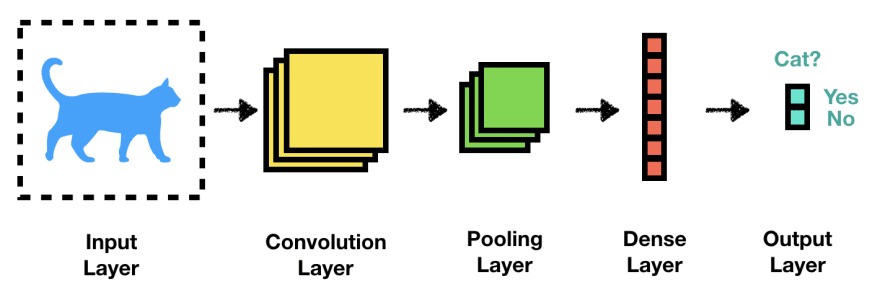
\includegraphics[width=15cm]{archivos/2.EstadoArte/CNNExample}
    \caption{Ejemplo de una red neuronal convolucional para una tarea de clasificación \cite{CNNExampleEAImage}.}
    \label{CNNExample}
\end{figure}


Uno de los principales inconvenientes comunes en estos estudios suele ser la baja calidad de los conjuntos de datos ofrecidos por las instituciones y el difícil acceso a los mismos \cite{ImportanciaDeBajaCalidadActualmenteDeDatasets}. Además, el desbalanceo de datos, asociado a la naturaleza del problema, genera una dificultad añadida a dichos estudios, ya que, en el caso de los accidentes de tráfico, gran parte de ellos suelen ser leves, siendo el número de accidentes serios y fatales mucho menor. Existen numerosos artículos que analizan este problema y se proponen distintas soluciones, como la utilización de técnicas de remuestreo \cite{ItalianoMetricasDesbalanceo} o la definición de nuevas métricas de clasificación.


Paralelamente a la predicción de gravedad de los accidentes de tráfico, existen múltiples variantes al problema que permitirían reducir el número de fallecidos en las carreteras aplicando distintas técnicas de \textit{deep learning}. Recientes investigaciones proponen arquitecturas complejas para crear mapas de riesgos de accidentes, tomando como entrada imágenes tomadas por satélite, segmentación de carreteras, información GPS de los vehículos y datos de accidentes con la finalidad de detectar las zonas más peligrosas
\cite{MIT}.	% Plantilla: Se muestran listas
%%%%%%%%%%%%%%%%%%%%%%%%%%%%%%%%%%%%%%%%%%%%%%%%%%%%%%%%%%%%%%%%%%%%%%%%
% Plantilla TFG/TFM
% Escuela Politécnica Superior de la Universidad de Alicante
% Realizado por: Jose Manuel Requena Plens
% Contacto: info@jmrplens.com / Telegram:@jmrplens
%%%%%%%%%%%%%%%%%%%%%%%%%%%%%%%%%%%%%%%%%%%%%%%%%%%%%%%%%%%%%%%%%%%%%%%%

\chapter{Tecnologías}
\label{3.Tecnologias}

    Una vez definido el problema a tratar, los objetivos generales y específios del proyecto, la solución propuesta y los requisitos a implementar hay que analizar las herramientas y tecnologías a utilizar. Para esto habrá que plantearse diferentes modelos y tecnologías disponibles para el desarrollo y optar por aquellos que aporten estabilidad y buen rendimiento.\\

    Cabe resaltar que el código implementado en este proyecto es completamente escalable y reusable. Esto permite que para adaptar este proyecto a otro problema distinto únicamente sea necesario realizar la limpieza correspondiente del conjunto de datos específico y definir las jerarquías de las categorías utilizadas.

    \section{Modelos}

        En primer lugar analizaremos los modelos utilizados durante la realización del proyecto.

        \subsection {Algoritmos Genéticos}
            Un \textit{Algoritmo Genético} \cite{GA}, es un modelo que imita la evolución de las especies en el ámbito de la biología, con el objetivo de encontrar una solución potencialmente óptima a un problema. El planteamiento de estos modelos consiste en evaluar los individuos pertenecientes a la población de la generación correspondiente para tomar el subconjunto de aquellas soluciones que mejor calidad ofrezcan mediante una función heurística denominada \textit{función fitness} que aproxima soluciones ideales a un problema.\\

            Hay que remarcar que las funciones heurísticas son funciones aproximadas a una solución ideal del problema, debido a que todas las posibles combinaciones de los parámetros a optimizar genera un espacio de búsqueda exponencial (problema NP-hard), es necesario crear una aproximación mediante la función heurística para acotar éste espacio.\\

            Para comprender el funcionamiento de los algoritmos genéticos es necesario analizar cada una de las fases que lo constituyen:
            
            \begin{enumerate}
                \item Inicialización de la Población:

                        En primer lugar es necesario generar los \textit{n} individuos de la población aleatoriamente. Cada uno de estos individuos está formado por el conjunto de variables que son objeto de optimización \ref{InitialPopulation}.

                        \begin{figure}[h]
                            \centering
                            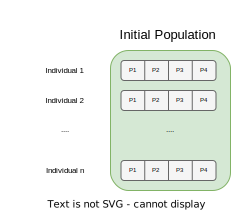
\includegraphics[width=6cm]{archivos/3.Tecnologias/GA/InitialPopulation}
                            \caption{Inicialización de la población. Cada individuo está constituido por n variables.}
                            \label{InitialPopulation}
                        \end{figure}

                \item Evaluación de Población:

                        Es la primera fase del proceso iterativo del algoritmo genético y, en él, cada uno de los individuos pertenecientes a la población son evaluados mediante la función \textit{fitness}.

                \item Selección de Padres:

                        Una vez evaluados los individuos de la población, se procede a seleccionar aquellos que mejor valor han obtenido para crear nuevas soluciones a partir de éstos padres. Existen distintas técnicas de selección, como por ejemplo escoger aquellos \textit{n} mejores padres de la población o técnicas basadas en métodos probabilísticos, para que aquellos individuos que menos puntuación logren, tengan alguna probabilidad de ser elegidos para la generación de nuevas soluciones. Este tipo de técnicas se utilizan para aumentar la diversidad en la pobĺación y evitar caer en soluciones acotadas a mínimos locales del problema. Se puede ver el proceso de cómo son seleccionados los padres en función de su \textit{fitness} en la figura \ref{FitnessFunction}.

                        \begin{figure}[h]
                            \centering
                            \hspace*{1in}
                            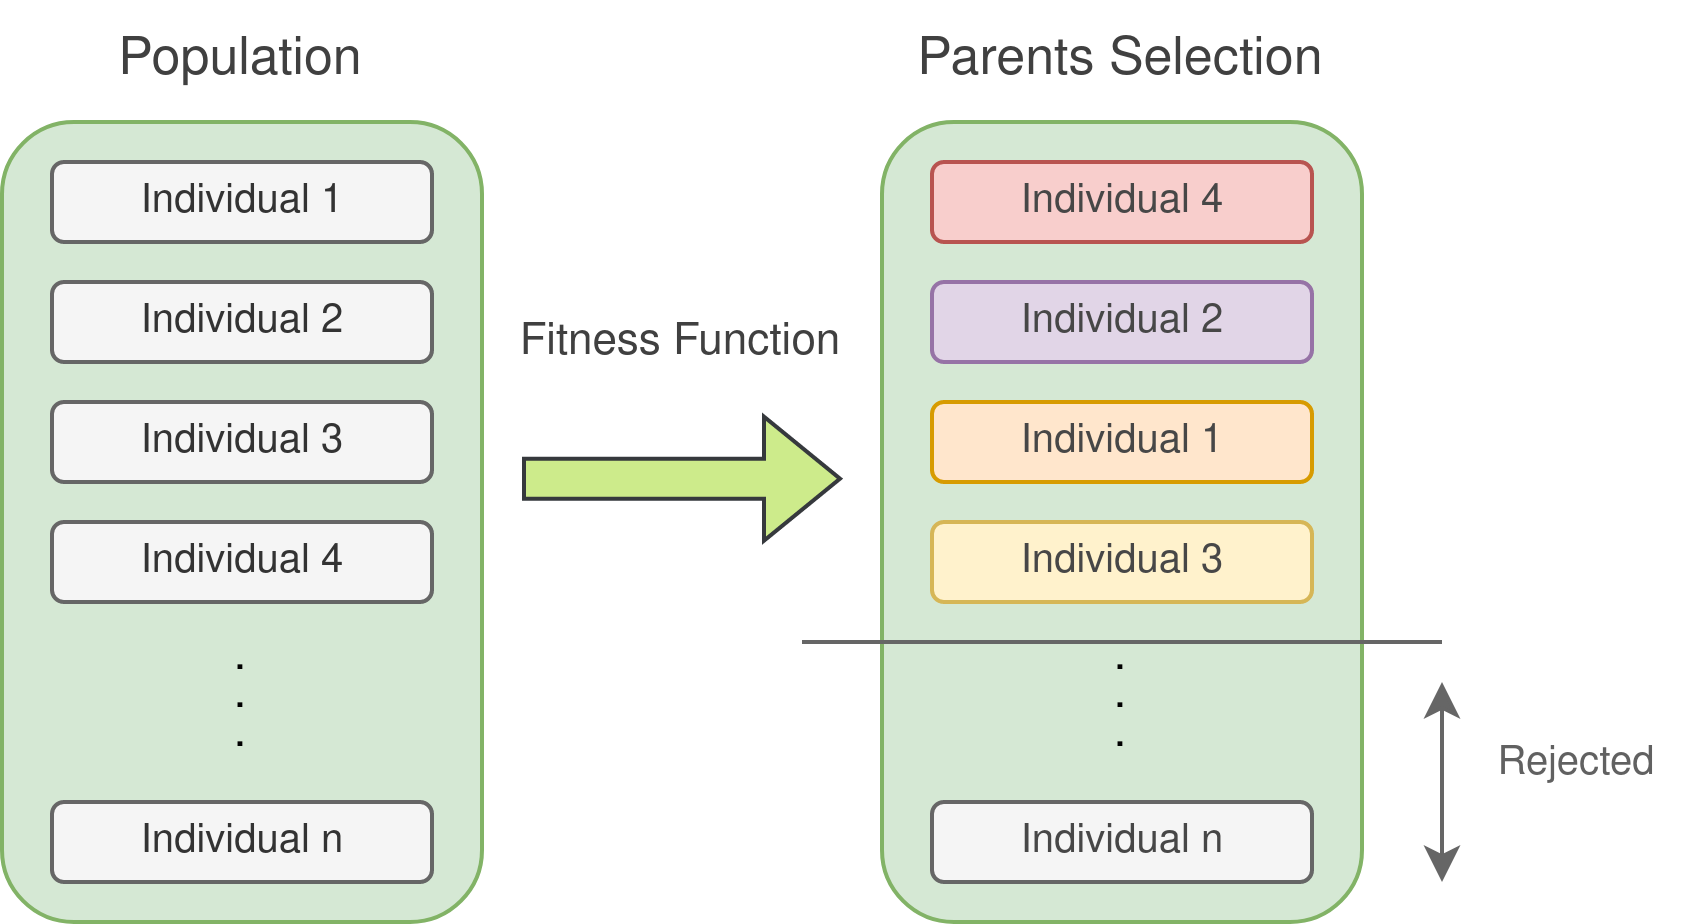
\includegraphics[width=10cm]{archivos/3.Tecnologias/GA/FitnessFunction}
                            \caption{Selección de padres candidatos.}
                            \label{FitnessFunction}
                        \end{figure}

                \item Cruce:

                        Una vez seleccionados los padres es necesario que intercambien información entre ellos para dar lugar a nuevos individuos, este proceso de herencia de información es posible realizarlo aplicando distintas filosofías; seleccionar un punto o posición de cruce a lo largo del vector de los padres y combinar ambos padres, o escoger aleatoriamente las posiciones de los parámetros de ambos padres y combinarlos para dar lugar a la solución generada figura [\ref{ParentsMatingMutationImage}].

                        \begin{figure}[h]
                            \centering
                            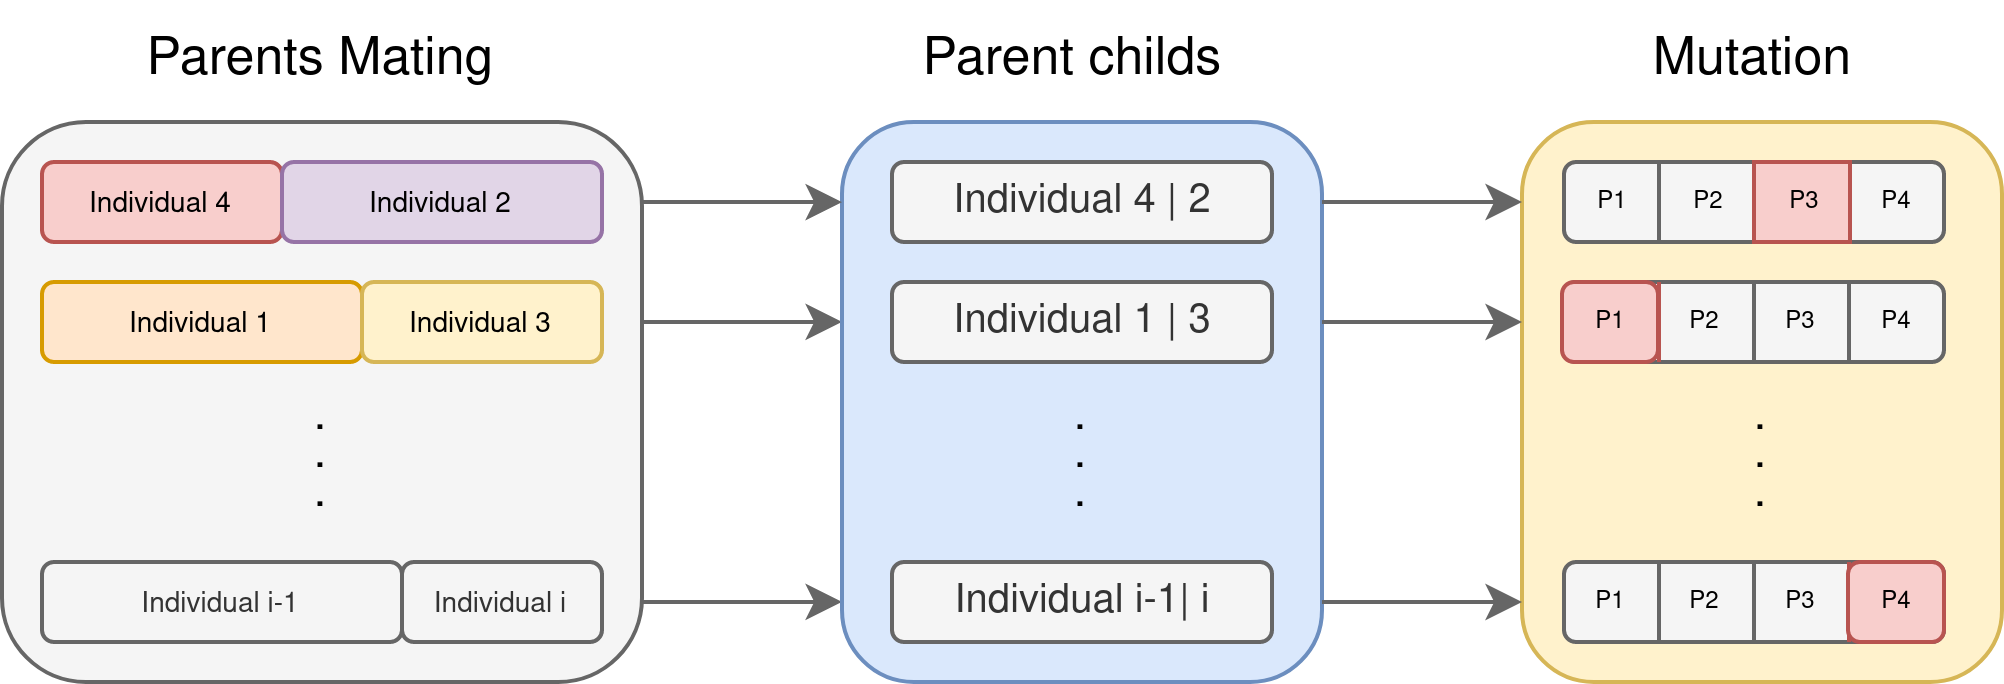
\includegraphics[width=12cm]{archivos/3.Tecnologias/GA/ParentsMatingMutation}
                            \caption{Procesos de cruce y mutación.}
                            \label{ParentsMatingMutationImage}
                        \end{figure}

                \item Mutación:

                        Cuando los padres seleccionados son combinados para dar lugar a los candidatos de la nueva generación, es importante aplicar un proceso de mutación entre éstos debido a la necesidad de generar diversidad en la población. Si se combina la misma información entre generaciones se corre el riesgo de converger prematuramente a un mínimo local del espacio de búsqueda. Por este motivo se introduce el concepto de mutación, que consiste en aplicar una modificación aleatoria sobre alguno de los parámetros de los individuos generados para poder ampliar el espacio de soluciones. 
            \end{enumerate}

            Cada una de las fases enumeradas anteriormente se repite de forma iterativa entre generaciones hasta que se cumpla alguna condición de parada.


            A continuación enumeraremos los parámetros con los que configurar un algoritmo genético. Dependiendo del tipo de algoritmo utilizado es posible encontrar distintos parámetros con los que inicializar el algoritmo, sin embargo estos son los más extendidos:


            \begin{itemize}


                \item Probabilidad de cruce: probabilidad con la que dos padres intercambian su información entre sí para dar lugar a un nuevo individuo hijo.

                \item Probabilidad de mutación: indica la probabilidad con la que cada hiperparámetro puede variar su valor.

                \item Tamaño de la población.

            \end{itemize}


        \subsection {XGBoost}

            
            \textit{Extreme Gradient Boosting Algortihm} (\textit{XGBoost}) es una libería open-source que implementa algoritmos \textit{ML Ensembles de tipo Boosting}. Se trata unos algoritmos muy utilizado en los últimos años, logrando un rendimiento superior a otras soluciones populares llegando a las primeras posiciones en numerosos retos propuestos en \textit{Kaggle} \cite{XGBoostTutorial}. Se basa en los modelos \textit{Ensemble Boosting} de los algoritmos de \textit{ML}, de ahí su nombre \textit{Gradient Boosting}. La técnica \textit{Boosting} se basa en construir un modelo robusto (\textit{strong learner}) combinando una serie de modelos débiles (\textit{weak learners}) \cite{NvidiaXGBoost}. Concretamente \textit{XGBoost} implementa \textit{Gradient Boosting Decision Trees (GBDT)}, que es un algoritmo similar a los \textit{Random Forest}, y es utilizado tanto para clasificación como para regresión.\\

            La diferencia principal entre los algoritmos \textit{Random Forest} y \textit{XGBoost} radica en el hecho de que los primeras utilizan algoritmos \textit{Ensembles} tipo \textit{Bagging} y construyen un modelo final predictivo mediante en el que la salida será la combinación de las predicciones de cada uno de los modelos individuales. En el caso de los modelos \textit{Ensembles Boosting} (\textit{XGBoost}) se combinan secuencialmente de forma que su objetivo es minimizar el error producido los árboles generales utilizando para ello el método de descenso por gradiente.\\


            En la figura [\ref{XGBoostFlowImage}] se puede observar cómo se van construyendo los árboles clasificadores y cómo cada árbol minimiza el residuo producido por el árbol anterior.\\


            \begin{figure}[h]
                \centering
                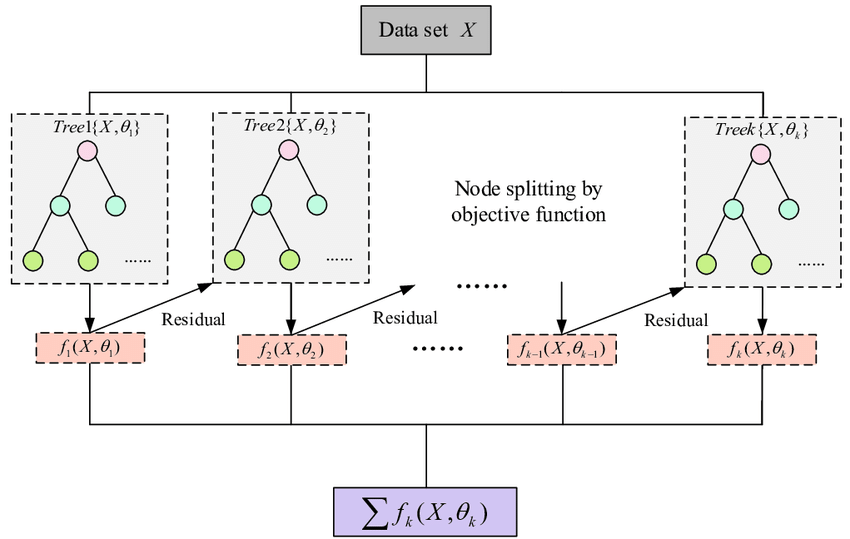
\includegraphics[width=10cm]{archivos/3.Tecnologias/XGBoost/XGBoostFlowImage}
                \caption{Proceso de optimización de XGBoost.}
                \label{XGBoostFlowImage}
             \end{figure}

            
            Además, \textit{XGBoost} aplica técnicas de regularización en su función de pérdida, de tal forma que reduce la influencia individual de cada árbol generado y de sus hojas para poder dar lugar a posteriores árboles que consigan mejorar el modelo, evitando de esta manera el sobreajuste u \textit{overfitting}.


        \subsection {\glsentrylong{gnb}}

        El clasificador probabilístico \glsentryfull{nb} es un modelo que se basa en el \textit{Teorema de Bayes}, este clasificador asume ciertas suposiciones de independencia sobre los predictores para realizar las clasificaciones. Se asume que la presencia o ausencia de cualquier predictor no está condicionada por la inclusión o exclusión de cualquier otro en el conjunto de datos, es decir, cualquier característica de las observaciones es independiente del resto. Asumiendo esta independencia entre los predictores la complejidad computacional del modelo se reduce considerablemente, haciendo de este modelo uno de los más eficientes en aprendizaje estadístico.\\

        Para utilizar este clasificador con valores reales se asume la distribución Gaussiana de las características, a esta adaptación se le denomina como \glsentryfull{gnb}. Este enfoque es más simple, ya que únicamente es necesario calcular la media y la desviación típica de las variables de entrada para resumir dichas distribuciones, que se utilizarán para calcular la probabilidad de pertenencia a una clase en función de estas distribuciones normales.\\

        El primer paso será calcular la denominada probabilidad a priori, que es la probabilidad de que una nueva muestra pertenezca a alguna de las clases del conjunto de entrenamiento, este cálculo serviŕá para determinar la predicción final de las observaciones. Posteriormente se calculará, para cada una de las variables de la muestra, la probabilidad de pertenecer a cada clase del conjunto de entrenamiento en función del grado de pertenencia a la distribución Gaussiana correspondiente a la variable. Después se aplicará esta multiplicación de probabilidades a la probabilidad a priori inicial definida a dicha clase.

        \subsection {\glsentrylong{svc}}


            Los \glsentryfull{svc}, también denominados como \textit{Soft Margin Classifier}, son modelos orientados a clasificación múltiple \cite{SVC}, que se basan en proyectar los datos de entrada en un espacio multidimensional buscando la separabilidad de estas muestras en este espacio.\\

            Los \glsentryshort{svc} construyen, lo que se denomina, hiperplanos en base a la máxima separabilidad de las clases utilizando únicamente aquellas observaciones que se encuentren en la fronteras que maximizan la distancia en el plano entre las clases. La ventaja de esta técnica es que es necesario un conjunto muy pequeño de muestras de entrenamiento para sostener los hiperplanos que forman las fronteras de decisión, estos puntos se denominan \textit{vectores de soporte}.\\

            La distancia entre los vectores de soporte y el hiperplano definido es denominado \textit{margen}, y es en este punto donde entra en juego la flexibilidad de los \glsentryshort{svc}. Estos modelos aplican el denominado \textit{margen blando}, que se basa en permitir que ciertas observaciones se encuentren en un lado erróneo del margen o incluso del hiperplano, haciendo que el modelo sea más robusto permitiendo mayor generalización a costa de clasificar erróneamente alguna de las observaciones mediante un parámetro de tolerancia $C$. A un mayor valor de $C$ se permite que un mayor número de muestras violen el margen \citep{ISLR2}.\\

            En la figura [\ref{SVCExampleImage}] se muestra un ejemplo aplicado de \glsentryshort{svc}, donde se observan los hiperplanos definidos que maximiza la separabilidad de ambas clases y los vectores de soporte definidos en función de distintos valores de tolerancia $C$.

            \begin{figure}[h]
                \centering
                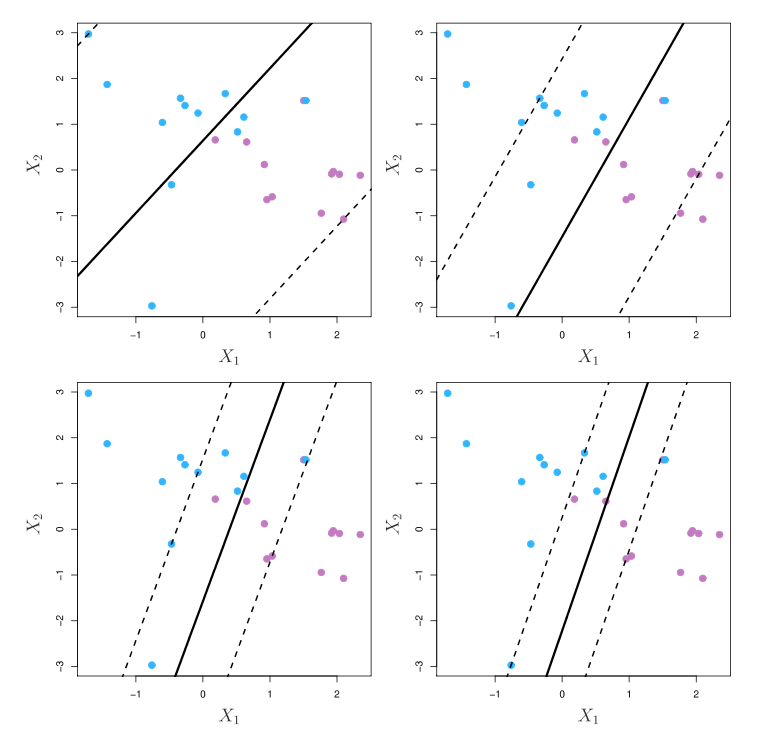
\includegraphics[width=10cm]{archivos/3.Tecnologias/SVC/SVCExample}
                \caption{ISLR2. Ejemplo de SVC con distintos valores de C.}
                \label{SVCExampleImage}
             \end{figure}

        \subsection {Redes Neuronales}

            Las Redes Neuronales (\glsentryshort{nn}) son modelos que emulan comportamiento del cerebro a la hora de procesar la información, entrenándose sobre un conjunto de datos para identificar patrones entre ellos \cite{NNReview}.\\

            A modo de comprensión, se muestra la arquitectura de una \textit{NN}, donde se pueden observar las conexiones entre cada capa de la red y sus salidas en la figura \ref{NNImage}. Existe una capa de entrada inicial que corresponde a cada una de las características del ejemplo de entrada. Cada una de las características de la capa de entrada se conecta con cada una de las neuronas de la primera capa oculta (\textit{hidden layer}) a través de conexiones denominadas pesos (\textit{weights}) que son los que serán aprendidos en la red con el objetivo de encontrar patrones entre las características. Esta metodología se aplica para cada una de las \textit{hidden layers} presentes en la arquitectura hasta la última capa que dictará la clase predicha en base a su salida (\textit{output layer}).\\

            \begin{figure}[h]
                \centering
                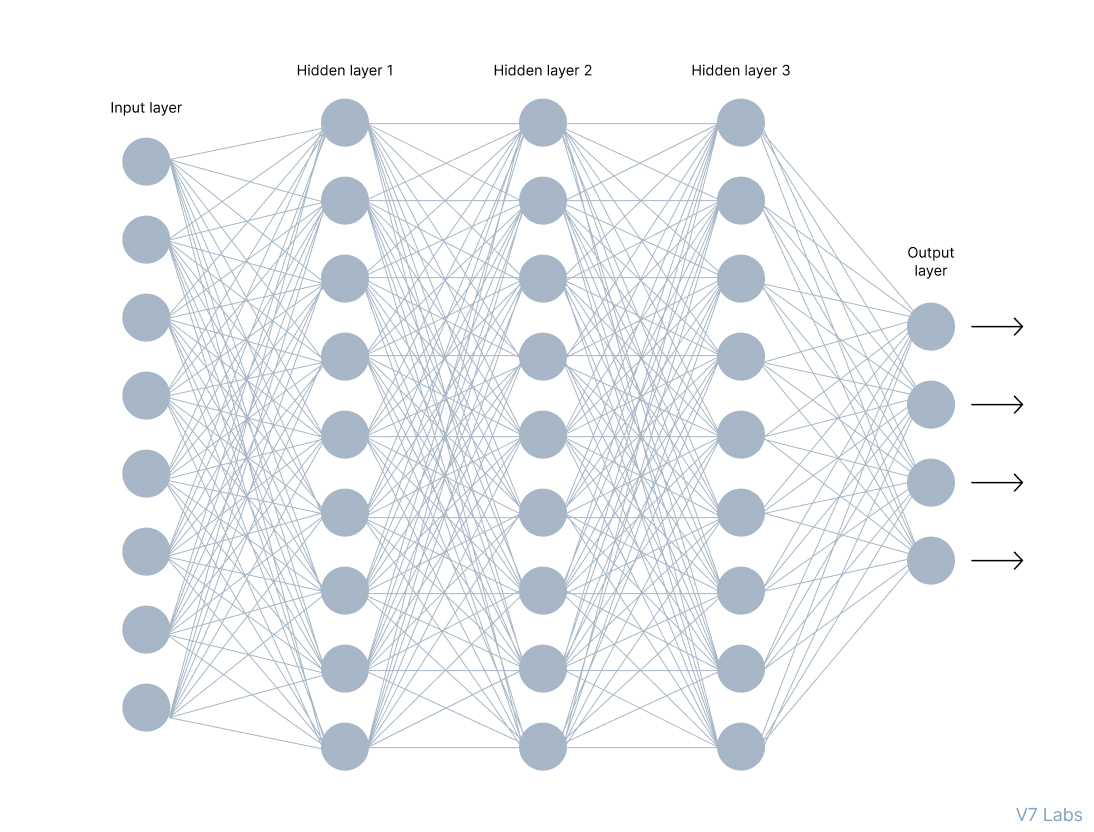
\includegraphics[width=10cm]{archivos/3.Tecnologias/RedesNeuronales/NNImage}
                \caption{Arquitectura de una Red Neuronal \cite{ReferenciaImagenNN}.}
                \label{NNImage}
             \end{figure}



            Existen una serie de conceptos comunes a todas las \textit{NN} que es conveniente nombrar para su comprensión:


            \begin{itemize}

                \item Función de activación: las funciones de activación son las encargadas de decidir si una neurona es activada o no en función de la entrada a esta función. Esta función suele situarse en la salida de cada capa de la red para decidir si una determinada neurona de la siguiente capa se activa o no. Existen distintos enfoques en lo que respecta a las funciones de activación, como la función logística, tangente hiperbólica y \textit{softmax} entre otras.

                \item Entropía: la entropía sobre una varible aleatoria $X$ es el grado de incertidumbre producido en base a los posibles valores que puede tomar como respuesta. Se calcula en base a la siguiente fórmula:

                    \begin{center}
                        $H(X) = -\sum_{i = 1}^n p(x_i) \log_2 p(x_i)$
                    \end{center}

                    Donde $x_i$ es cada uno de los posibles valores que puede tomar la variable como respuesta y $p(x_i)$ es la probabilidad de obtener dicho valor. 


                \item Softmax: se trata de la generalización en forma multidimensional de la función logística o \textit{logistic function}. \textit{Softmax} es una función que permite la transformación de un vector de números reales a una distribución de probabilidad. Esta función se suele aplicar como capa de activación en el último nivel en las \textit{NN}, representando la probabilidad de que la salida de la red pertenezca a cada una de las $K$ clases posibles en el modelo \cite{Softmax}. 

                Esto es necesario debido a que normalmente los componentes de la salida de la última capa de una red neuronal (\textit{logits}) son el resultado de la predicción en forma de números reales no normalizados, por lo tanto pueden ser mayores que $1$ e incluso negativos. La función permite calcular la distribución de probabilidad en base a estos \textit{logits} y calcular la probabilidad de pertenencia de la muestra a cada una de las $K$ clases que componen el modelo.

                \item Cross-Entropy: el objetivo de cross-entropy es minimizar la función de pérdida (\textit{log loss}) comparando la probabilidad de la clase predicha con respecto a su valor verdadero. Al aplicar una penalización logarítmica, las probabilidades de las clases que más disten respecto a su valor verdadero se verán más acentuadas \cite{Cross-Entropy}.

                \begin{figure}[h]
                    \centering
                    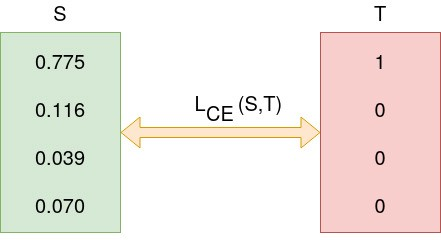
\includegraphics[width=7cm]{archivos/3.Tecnologias/RedesNeuronales/CrossEntropy}
                    \captionsetup{width=.65\textwidth}
                    \caption{Cross-Entropy entre la función Softmax (izquierda) y el valor de la clase verdadera (derecha) \cite{Cross-Entropy}.}
                    \label{CrossEntropyImage}
                 \end{figure}

                \item Back Propagation: en el proceso de entrenamiento de la \textit{NN} es necesario actualizar los pesos de las capas ocultas con el objetivo de minimizar la cross-entropy total del modelo. Para minimizar este valor se utiliza el algoritmo de optimización descenso por gradiente.

                Gracias a las propiedades de la función \textit{Softmax} es posible utilizar descenso por gradiente para calcular la derivada de la función de pérdida respecto de cada uno de los pesos de las capas intermedias de la red y actualizar cada uno de ellos con el objetivo de minimizar la función de pérdida.

                \item Learning Rate: es la \textit{tasa de aprendizaje} que define el tamaño de paso que se aplicará a la hora de optimizar los pesos de la red. Su valor está en el intervalo $[0,1]$, de tal forma que a menor valor de la tasa de aprendizaje menor será el cambio que se produce en los pesos de las neuronas del modelo. Este parámetro no es sencillo de especificar, el \textit{learning rate} es un regularizador que con valores altos permite que la red no caiga en \textit{overfitting}, caso que ocurriría si el valor fuera demasiado pequeño y la minimización de la función de pérdida cayese en un mínimo local debido a aprender demasiado de los datos de entrenamiento. Si el valor es muy alto los pesos de los parámetros de la red variarán excesivamente impidiendo la convergencia en un mínimo de la función. Esta disyuntiva ha sido ampliamente estudiada en los últimos tiempos, acerca de cuál es el valor ideal del \textit{learning rate} en las \textit{NN} \cite{LearningRate}, aunque comunmente se configura con el valor $0.1$.

                \item Batch Normalization: el proceso de entrenamiento de una red neuronal puede ser costoso, ya que existen una gran cantidad de parámetros para cada capa que son optimizados durante el proceso de entrenamiento. Esto hace que este proceso sea demasiado sensible a los parámetros inicializados en el inicio del entrenamiento de la red, como es el ejemplo de establecer una tasa de aprendizaje \textit{learning rate} muy baja para poder converger. Esto hace que el entrenamiento sea muy lento, por lo que es necesario normalizar las entradas para cada mini-batch (subconjuntos de datos de entrenamiento con el que se entrena la red en cada época. El método \textit{Batch Normalization} \cite{BatchNormalization} normaliza los datos de tal forma que permite utilizar tasas de aprendizaje mayores además de actuar como regularizador, reduciendo así el número de capas \textit{Dropout} que pudieran existir en la arquitectura.

            \end{itemize}

            Existe una clase de redes neuronales, denominadas redes neuronales convolucionales, con uana serie de parámetros específicos. En concreto las redes neuronales convolucionales 1D o 2D tienen las siguientes:

                \begin{itemize}

                    \item Kernels:

                        Son las estructuras que se encargan de realizar la convolución. Los kernels son matrices de pesos unidimensionales ($1 \times n$) o bidimensionales ($n \times m$) dependiendo del tipo de convolución que se esté aplicando (Convolución 1-D o Convolución 2-D), y se encargan de inferir patrones en la matriz de entrada gracias a la actualización de sus pesos. En función de la profundidad de la capa, los kernels podrán encontrar patrones más simples o más complejos debido a que la entrada a cada capa es una convolución (aplicación del filtro) de las capas anteriores.

                        Un kernel realiza el producto escalar de sus pesos con respecto a las posiciones de la matriz de entrada (imagen o \textit{feature map}) que colisionen en ese momento con el kernel, generando un nuevo \textit{feature map} de menor dimensión, a menos que se utilice la técnica de \textit{Padding} \cite{Kernels}.
                         
                    \item Filtros:

                        Un filtro no es más que una agrupación de kernels, siempre tendrán una dimensión mayor que la definida para el kernel. Por ejemplo, si disponemos de un kernel unidimensional ($1 \times n$), el filtro contendrá $k$ kernels de ($1 \times n$) en la capa convolucional definida \cite{FiltersFeatureMaps}

                    \item Strides:

                        Son los saltos producidos por un kernel en cada etapa de la convolución, dependiendo si la convolución es dimensional o bidimensional, el stride constará de una dimensión ($i$), es decir, los pasos hacia la derecha en la matriz, o de dos dimensiones ($i, j$), los pasos hacia la derecha y hacia abajo en la matriz.

                        \begin{figure}[h]
                            \centering
                            \captionsetup{width=.65\textwidth}
                            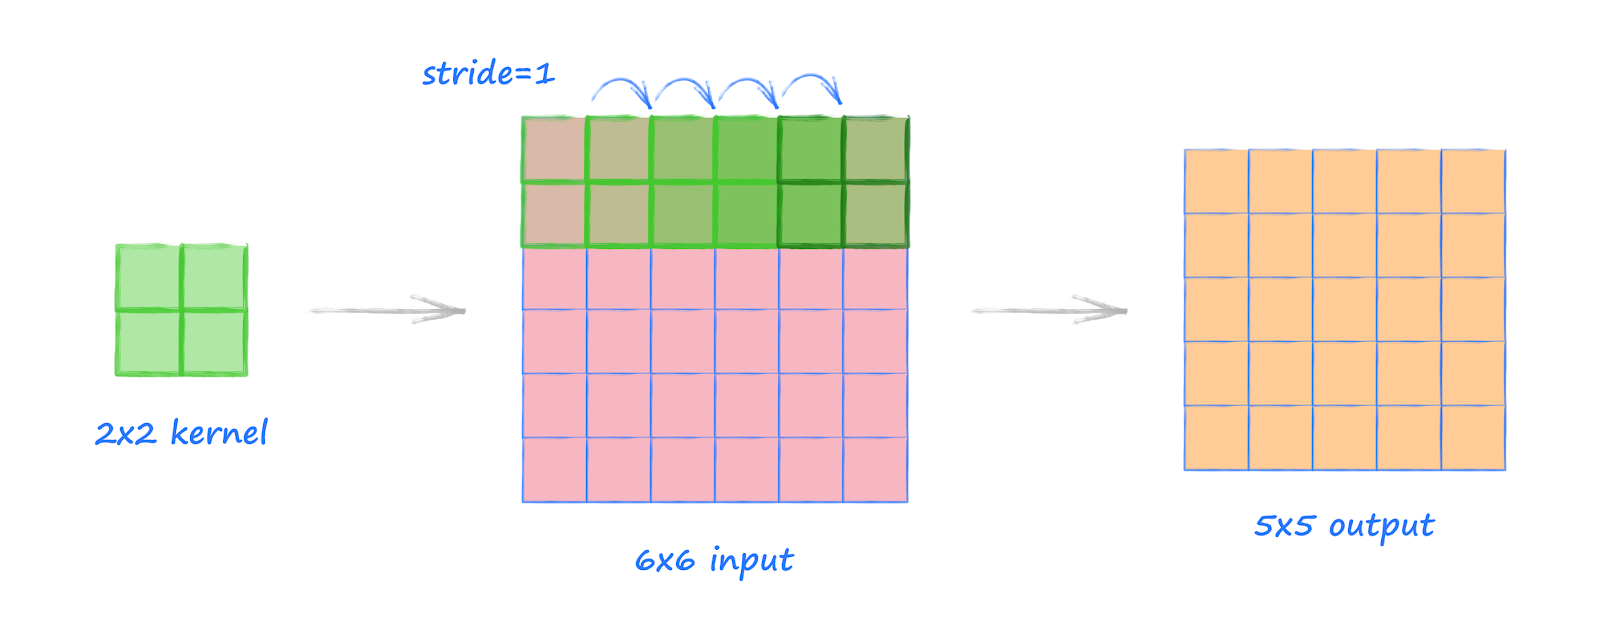
\includegraphics[width=10cm]{archivos/3.Tecnologias/RedesNeuronales/Stride}
                            \caption{Aplicación de un kernel de dimensión 2x2 a una matriz con stride = 1 \cite{ReferenciaImagenStrides}.}
                            \label{StrideImage}
                         \end{figure}

                    \item Padding:

                        El padding es un método utilizado para incrementar la dimensionalidad de la entrada de la capa debido el desvanecimiento de los valores posicionados en zonas comprometedoras una vez aplicada la convolución. El \textit{padding} es el proceso de generar celdas artificiales inicializadas con valor \textit{0} que permiten que el filtro convolucional sea aplicado en su totalidad en la posición de estas zonas comprometedoras, manteniendo la información de los límites de la imagen. De otra forma ĺos valores de estos extremos se desvanecerían a medida se incrementa la profundidad de la red (número de capas) con respecto al resto de valores de la matriz.\\

                        \begin{figure}[h]
                            \centering
                            \captionsetup{width=.65\textwidth}
                            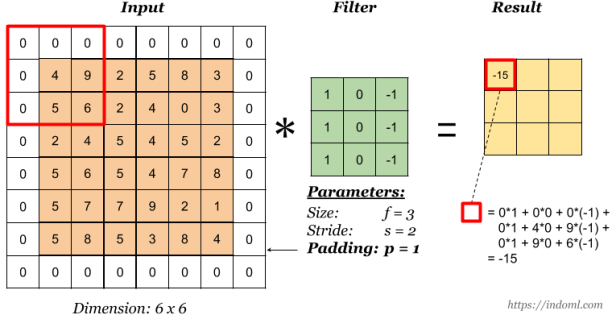
\includegraphics[width=10cm]{archivos/3.Tecnologias/RedesNeuronales/CNN/padding}
                            \caption{Proceso de convolucion de un kernel 3x3 sobre una entrada de 6x6 aplicando padding \cite{ReferenciaImagenKernelFiltro}.}
                            \label{PaddingImage}
                         \end{figure}


                    \item Función de activación:


                        En el caso de las redes neuronales convolucionales, la función de activación se aplica a cada casilla proyectada por cada kernel sobre la matriz de entrada, de tal forma que cambia el valor a $0$ sobre aquellos valores que resulten negativos de la convolución. En la figura \ref{CNNRELUImage} se puede apreciar cómo se aplica la función de activación \textit{ReLU} para cada casilla de la proyección de un \textit{kernel} bidimensinoal sobre una \textit{red convolucional de dos dimensiones}.



                        \begin{figure}[h]
                            \centering
                            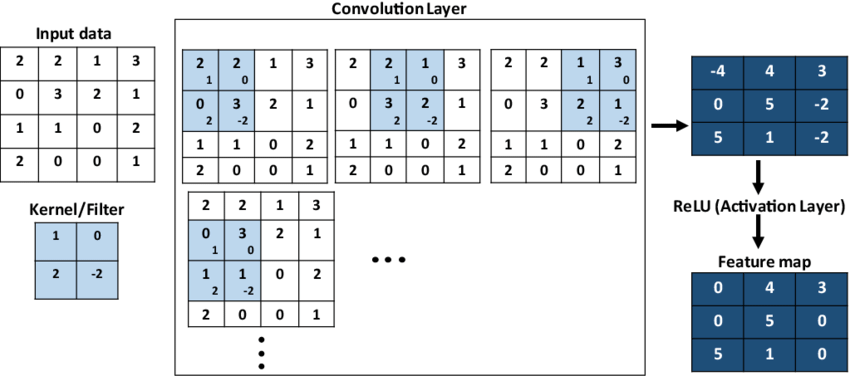
\includegraphics[width=10cm]{archivos/3.Tecnologias/RedesNeuronales/CNN/CNNRELUImage}
                            \caption{Ejemplo de ReLU aplicado a una convolución de dos dimensiones \cite{CNNReLUImage}.}
                            \label{CNNRELUImage}
                         \end{figure}

                \end{itemize}

                En el proceso de entrenamiento de las \textit{CNNs} cada uno de los valores de los kernels son optimizados mediante el método \textit{GD}, de tal forma que los pesos de cada capa son actualizados gracias a la derivabilidad de la función de pérdida.\\
                                
                Una \textit{Red Neuronal Convolucional de 1 Dimensión}, o \textit{Convolutional Neural Network 1-Dimensional (CNN-1D)}, es un tipo de red convolucional que utiliza kernels \textit{(filters)} que son aplicados a las matrices de entrada con el objetivo encontrar ciertas características en ellas.\\

                La baja carga computacional de estas arquitecturas las hacen atractivas para aplicarlas en tiempo real en dispositivos con pocos recursos como teléfonos móviles \cite{Conv1D_Survey}. Sin embargo, la complejidad computacional de las \textit{CNN-1D} puede ser mayor que la de las \textit{CNN-2D} debido a que necesitan desplazarse con un kernel generalmente más pequeño por la entrada de la red, además, estas redes se han demostrado ser más efectivas en distintos campos con respecto a las \textit{CNN-2D}, como en técnicas de análisis de señales.

                El resultado de este proceso es la proyección del filtro sobre un espacio dimensional denominado mapa de caracerísticas \textit{(feature maps)}. Este filtro se utiliza para convolucionar los feature maps de la capa anterior \cite{FiltersFeatureMaps} o de la imagen de entrada si se trata de la primera capa de la red.
                

                \begin{figure}[h]
                    \centering
                    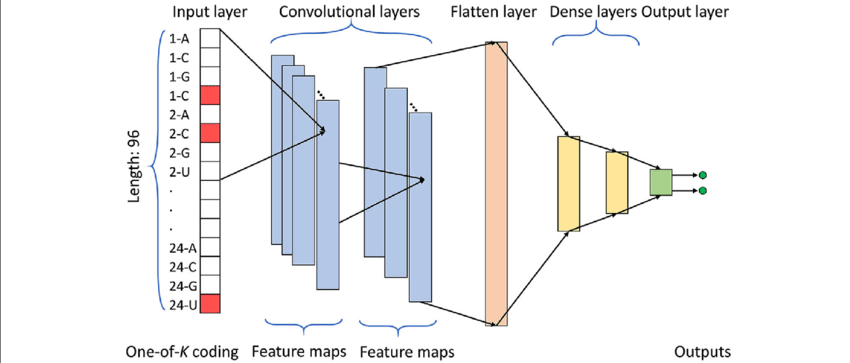
\includegraphics[width=8cm]{archivos/3.Tecnologias/RedesNeuronales/CNN/1D/1CNNArchImage}
                    \captionsetup{width=.7\textwidth}
                    \caption{Arquitectura de una red convolucional de una dimensión con dos capas convolucionales y una salida \cite{CNN1DArchitectureImage}.}
                    \label{1CNNArchImage}
                \end{figure}


                Al ser una arquitectura unidimensional, el \textit{kernel} tendrá que tener un tamaño ($1 \times n$).

                \begin{figure}[h]
                    \centering
                    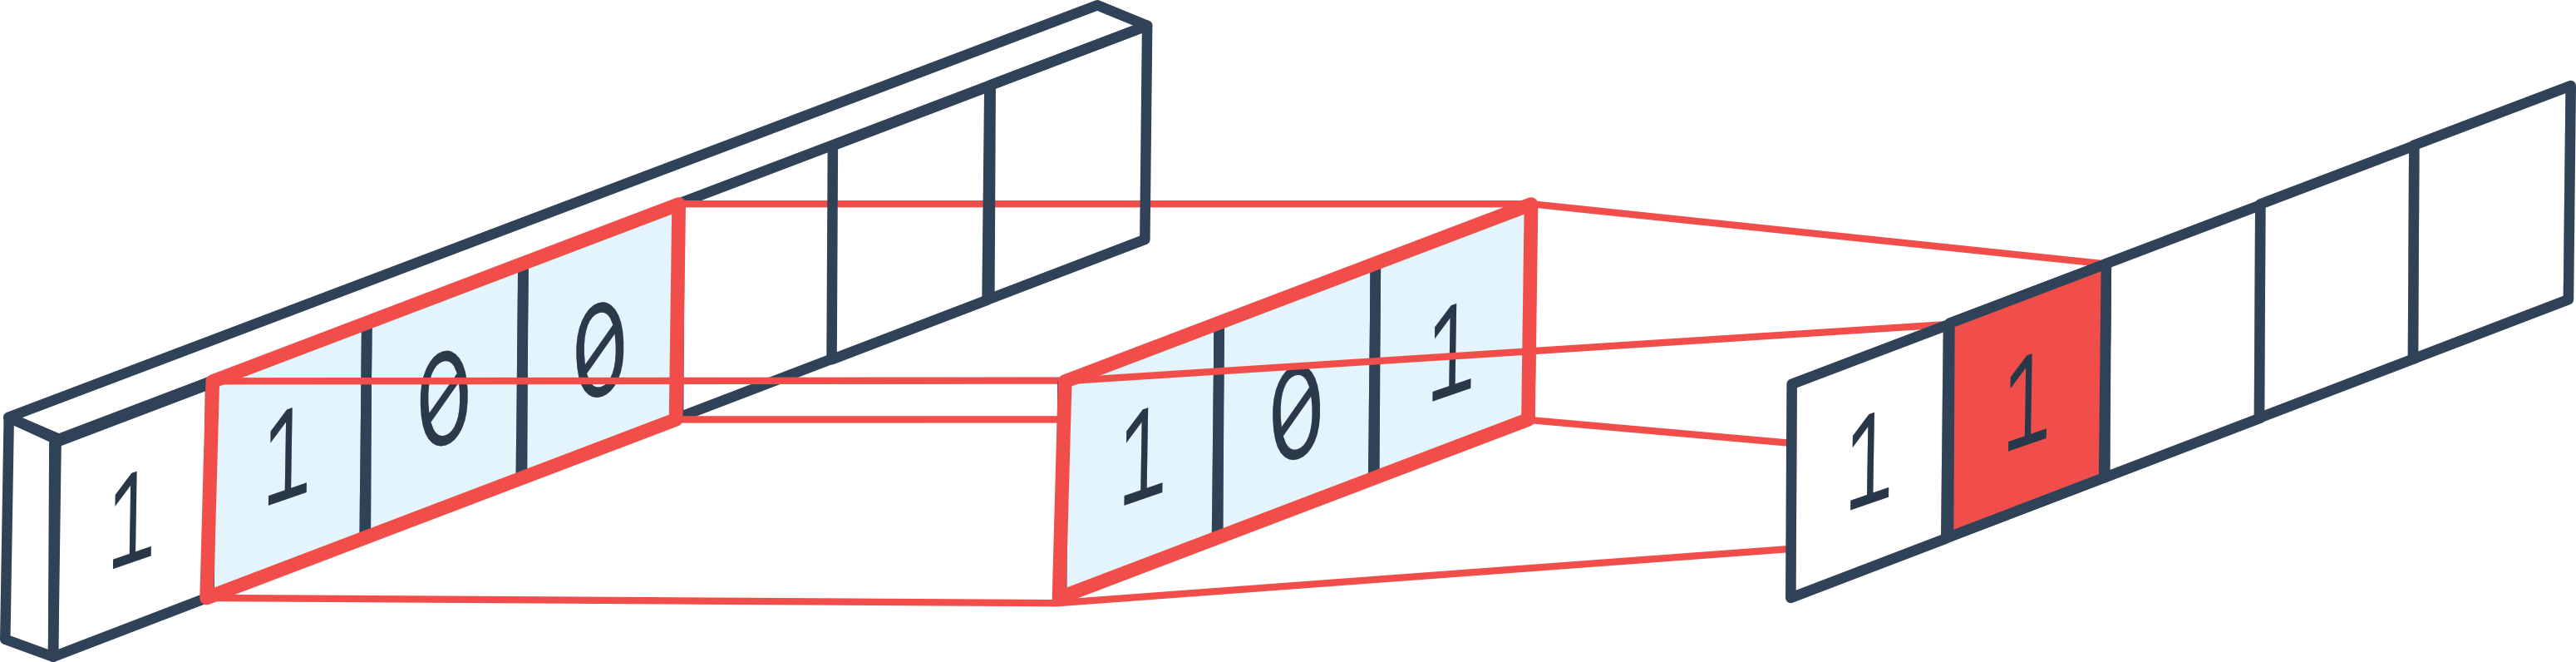
\includegraphics[width=7cm]{archivos/3.Tecnologias/RedesNeuronales/CNN/1D/1DConvolution}
                    \captionsetup{width=.75\textwidth}
                    \caption{A la entrada de la red (izquierda) se aplica un kernel (en el centro) que resulta en la convolución de un mapa de características (derecha) \cite{CNN1DImage}.}
                    \label{1DConvolutionImage}
                \end{figure}

                    
                Las técnicas convolucionales implementadas en este proyecto son las \textit{Redes Neuronales Convolucionales de 2 Dimensiones}, o \textit{Convolutional Neural Networks 2-Dimensional (CNN-2D)}. Al igual que en el caso de las \textit{CNN-1D}, el filtro se aplica sobre el input de la capa, resultando en \textit{feature maps}, sin embargo, en este caso \textit{kernel} será de bidimensional al ser una convolución de dos dimensiones, por lo que es necesario especificar el tamaño de la matriz que recorrerá la matriz pasada como entrada a la capa correspondiente.

            \subsection {\glsentrylong{knn}}

                El algoritmo \textit{K vecinos más próximos}, o \glsentryfull{knn} \cite{KNN}, es una técnica de aprendizaje supervisado ampliamente utilizada para tareas de clasificación y regresión. Es uno de los algoritmos básicos del aprendizaje automático y tiene una gran importancia en el campo de la \textit{Ciencia de Datos} debido a su simplicidad de implementación y a su interpretabilidad.\\

                El algoritmo \textit{KNN} asume que muestras con características parecidas deben pertenecer a la misma clase. O lo que es lo mismo, muestras parecidas deben estar cercanas en el espacio dimensional. Esta técnica se basa en representar las muestras de un conjunto de datos en base a sus características en un espacio n-dimensional y se basa en la suposición de que los vecinos más cercanos dan una. Normalmente la distancia empleada es la \textit{Euclídea}, aunque es posible calcular otras distancias como \textit{Manhattan} o \textit{Chebyshev}. A medida que se incrementan las dimensiones del espacio resulta más costoso computacionalmente calcular distancias entre los puntos.\\


                Por lo tanto, el único parámetro a configurar es el número de vecinos más cercanos que se calculará en base al punto que queramos clasificar, en la figura \ref{KNNImage} se muestra un ejemplo de un problema de clasificacíón aplicando distintos valores al parámetros $k$.

                \begin{figure}[h]
                    \centering
                    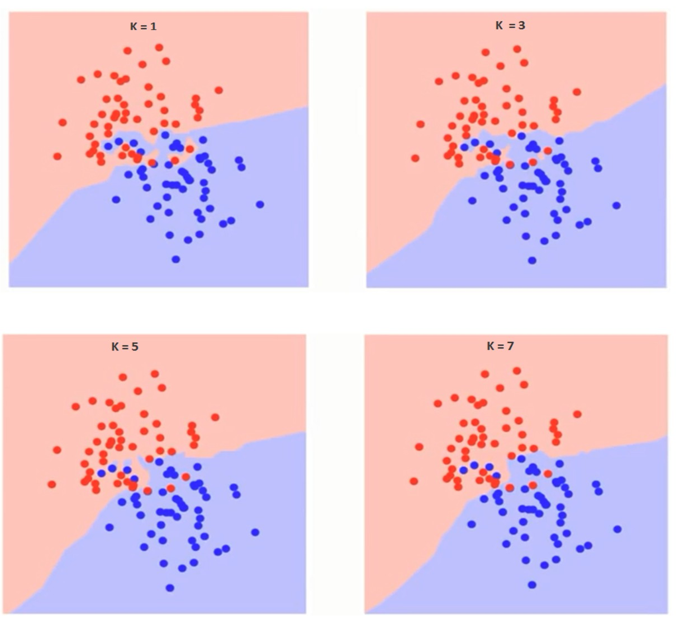
\includegraphics[width=10cm]{archivos/3.Tecnologias/KNN/KNNImage}
                    \captionsetup{width=.75\textwidth}
                    \caption{KNN aplicado con distintos valores de $k$ \cite{ReferenciaKNNImagen}.}
                    \label{KNNImage}
                \end{figure}

            

    \section{Especificaciones técnicas}

        En esta sección detallaremos las herramientas que han sido utilizadas para poder realizar este proyecto.


        \subsection{Herramientas utilizadas}
            En primer lugar se ha utilizado de forma intensiva \textit{Python}, que es un lenguaje de programación interpretado de nivel alto multiparadigma. La versión empleada para el desarrollo del proyecto ha sido 3.9.11 \cite{Python}. Dentro de este lenguaje de programación, las librerías más utilizadas han sido:

            \begin{description}

                \item Pandas: provee de herramientas que permiten el análisis y la manipulación de datos. La versión utilizada para este proyecto es la 1.3.5 \cite{Pandas}.

                \item Tensorflow: utilizada para la implementación de redes neuronales permitiendo su ejecución. Este proyecto se basa en la versión 2.8.0 \cite{Tensorflow}.

                \item Sklearn: contiene múltiples modelos predictivos implementados, basado en NumPy, SciPy y Matplotlib. La versión configurada para este proyecto es 1.0.2 \cite{Scikit-Learn}.

                \item XGboost: contiene la implementación del algoritmo XGBoost, además de múltiples configuraciones como la ejecución en \textit{CPU, GPU y GPU paralelizada}. La importación de esta librería ha sido en base a la versión 1.5.0 \cite{XGBoostLibrary}.

            \end{description}

            Respecto a otras herramientas \textit{Software} utilizadas destacan:

            \begin{description}

                \item CUDA: plataforma de computación paralelizada que permite la ejecución de código en \textit{GPU}, esto permite que las redes neuronales puedan entrenarse con mayor rapidez que en \textit{CPU} debido a la velocidad con la que se realizan las operaciones orientadas a datos en las tarjetas gráficas. Se ha utilizado la versión 11.6 \cite{CUDA}.

                \item Anaconda: distribución open-source que ofrece la flexibilidad de mantener varios entornos con distintas configuraciones y versiones de distinas librerías, facilitando además la migración entre equipos. La versión utilizada ha sido la 4.12.0 \cite{Anaconda}.

                \item Jupyter Notebook: entorno interactivo que permite la creación, edición y ejecución de notebooks de forma local y remota. La versión utilizada para el desarrollo de este proyecto ha sido la 6.4.10 \cite{JupyterNotebook}.

                \item Jupyter Lab: interfaz de nueva generación que convive con el entorno Jupyter Notebook, ofrece numerosas funcionalidades como es la navegación entre distintos repositorios dentro de la interfaz. La versión instalada para la realización del proyecto ha sido la 3.3.2 \cite{JupyterLab}.

                \item DiagramsNet: plataforma utilizada para la confección de figuras mostradas en este documento \cite{DiagramsNet}. 

                \item Google Meets: plataforma utilizada para realizar reuniones semanales con el tutor \cite{GoogleMeet}.

            \end{description}

            Como sistema de control de versiones se ha utilizado \textit{Github} \cite{Github}, repositorio donde es posible subir versiones del proyecto.

        \subsection{Especificaciones del servidor}
            La mayor parte de los experimentos realizados en este trabajo se han ejecutado bajo un servidor con CPU \textit{Dual AMD Rome 7742} (128 cores) y contando con una GPU \textit{DGX NVIDIA A100} de  40 GigaBytes (\textit{GB}).
            	% Plantilla: Se muestran figuras
%%%%%%%%%%%%%%%%%%%%%%%%%%%%%%%%%%%%%%%%%%%%%%%%%%%%%%%%%%%%%%%%%%%%%%%%
% Plantilla TFG/TFM
% Escuela Politécnica Superior de la Universidad de Alicante
% Realizado por: Jose Manuel Requena Plens
% Contacto: info@jmrplens.com / Telegram:@jmrplens
%%%%%%%%%%%%%%%%%%%%%%%%%%%%%%%%%%%%%%%%%%%%%%%%%%%%%%%%%%%%%%%%%%%%%%%%

\chapter{Metodología}
\label{metodologia}

El desarrollo de este proyecto respeta tanto el proceso de desarrollo \textit{Software} como el ciclo de vida de proyectos de \textit{Ciencia de Datos}, por lo que se ha dividido en varias fases acontecidas que definiremos a continuación en base a la planificación mediante un \textit{Diagrama de Gantt}:

Este diagrama proporciona una visión de las fases de un proyecto y su estimación temporal. En el caso que nos ocupa, el diagrama se muestra en al figura \ref{GranttImage}.
\begin{figure}[H]
    \centering
    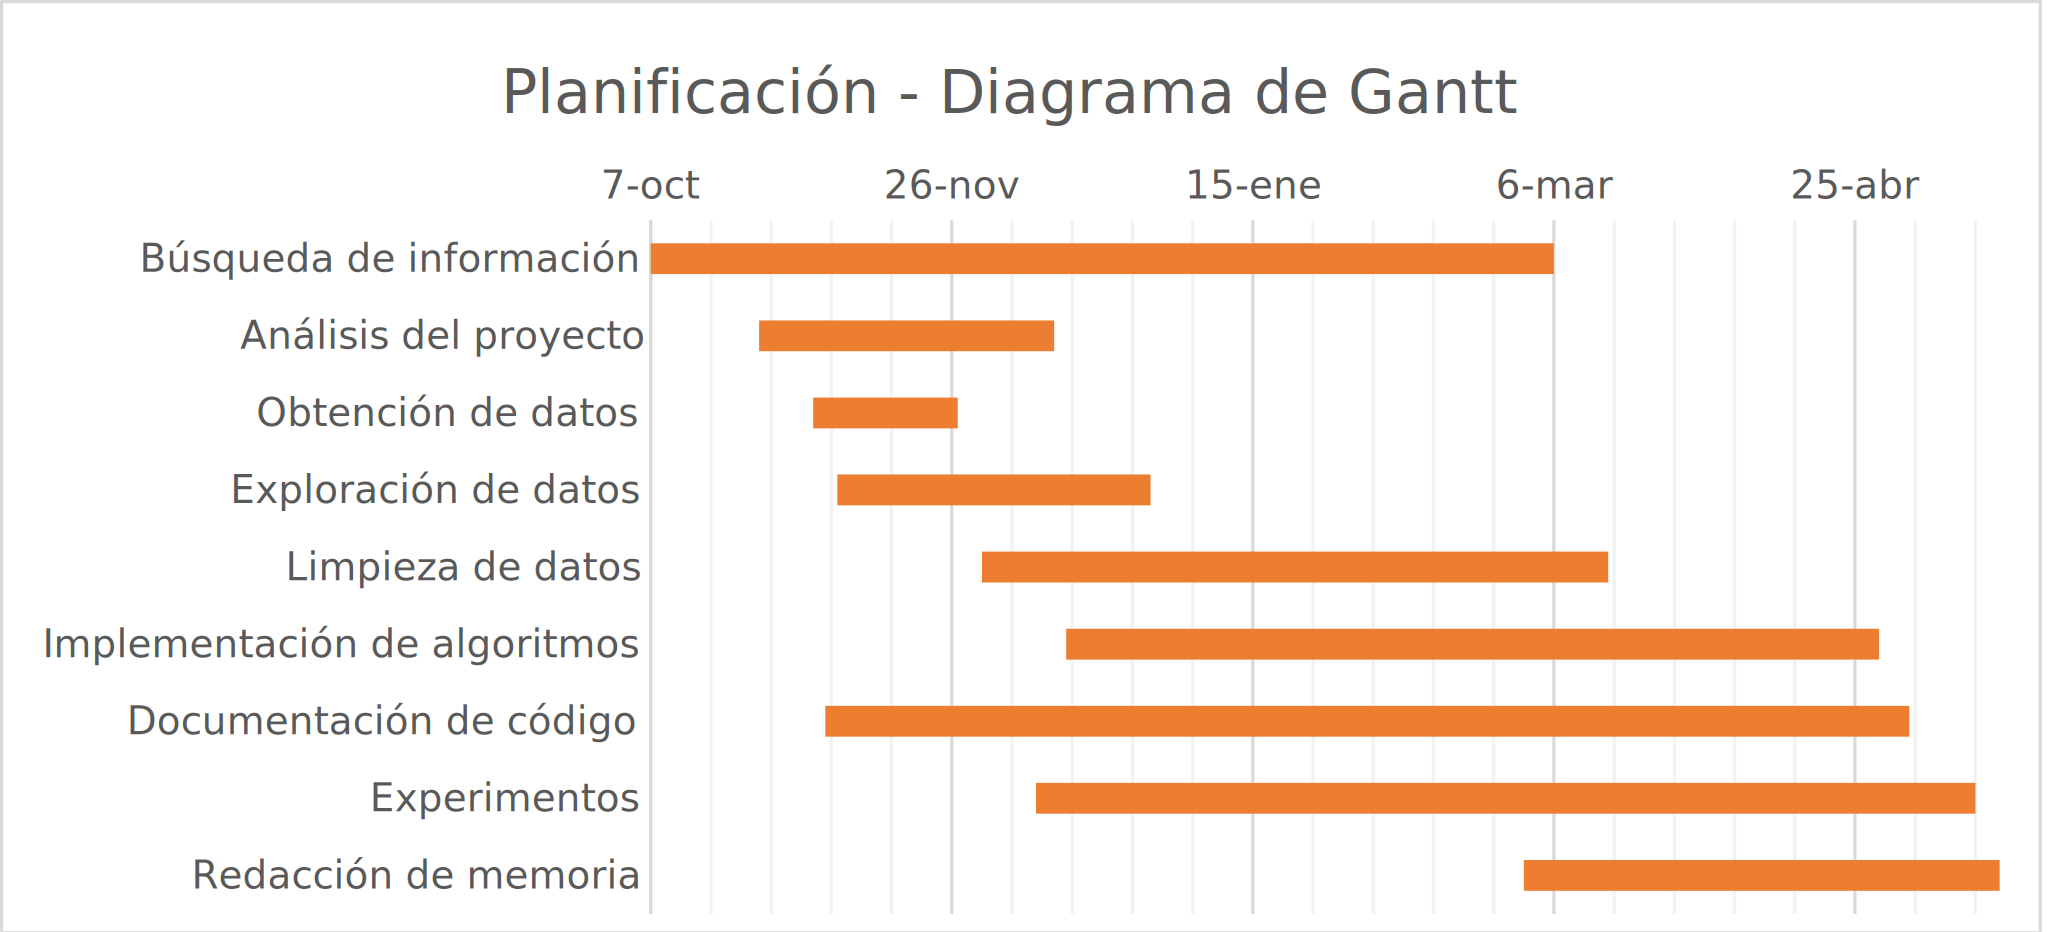
\includegraphics[width=15cm]{archivos/4.Metodologia/GranttImage}
    \caption{Diagrama de Gantt de la planificación del proyecto.}
    \label{GranttImage}
\end{figure}

La búsqueda de información incluye la investigación de todo lo referente al proyecto, y por este motivo, esta fase, es la primera en el desarrollo siendo un proceso que se ha prolongado durante casi toda la evolución del trabajo.

El análisis del proyecto consiste en estudiar la viabilidad del mismo, buscando fuentes de información desde las que poder obtener los datos además de explorarlos. Es una de las fases más críticas en un proyecto \textit{Data Science} ya que si las conclusiones del estudio de viabilidad no son sólidas, se podría cometer el riesgo de empezar un proyecto en el que no es factible cubrir los objetivos.

La obtención de datos consiste en la búsqueda de repositorios donde encontrar datos que contengan la información requerida para abarcar los objetivos del proyecto. Se ha realizado visitando distintos portales de datos abiertos nacionales hasta encontrar un conjunto de datos que encajase con los objetivos, en esta fase también se involucra la exploración inicial de los datos.

La exploración de datos abarca la fase de análisis de datos, esto se realiza utilizando métodos visuales para entender las características propias del dataset, además de hacer una valoración de la calidad de los mismos. Las primeras etapas de esta fase se complementan con el análisis del proyecto.

El siguiente paso ha sido la limpieza de datos, gracias a la exploración se comprenden la naturaleza de los datos y se decide qué tecnicas usar para el tratamiento de valores atípicos del conjunto de datos para su posterior transfomación.

Una de las tareas más importantes en el ciclo de vida de desarrollo Software que garantizan la calidad del producto es la documentación de código. Tiene como fin
clarificar conceptos y explicar el funcionamiento de los métodos que componen el desarrollo. Es una fase que se prolonga desde el inicio de la codificación en la limpieza de datos hasta poco tiempo después de terminar de implementar los modelos.

La última fase de este proyecto a nivel funcional de este proyecto ha sido la realización de experimentos, comienza poco antes que la implementación de los modelos y consiste en testar las distintas implementaciones, tanto de limpieza de datos como el funcionamiento de los modelos.

Finalmente hay que redactar la memoria, plasmando toda la información obtenida durante la evolución del proyecto.



\section{Proceso}

    \textbf{Nota: No me ha quedado del todo claro si el siguiente párrafo se posiciona aquí o hay que eliminarlo}
    En esta sección describiremos cada uno de los pasos que ha seguido el desarrollo del proyecto, desde la búsqueda inicial de datos hasta la implementación final de los algoritmos.

    Un aspecto muy importante en un TFM es el diagrama de flujo de la metodología. En este diagrama se define el flujo de ejecución del proyecto y, como se puede observar en la figura \ref{DataflowImage}, se han dividido las etapas del proyecto en seis bloques claramente diferenciados. Cada uno de estos está orientado a una disciplina distinta en proyectos de \textit{Ciencia de Datos} y por lo tanto serán detallados en cada una de las subsecciones posteriores.


    \begin{figure}[H]
        \centering
        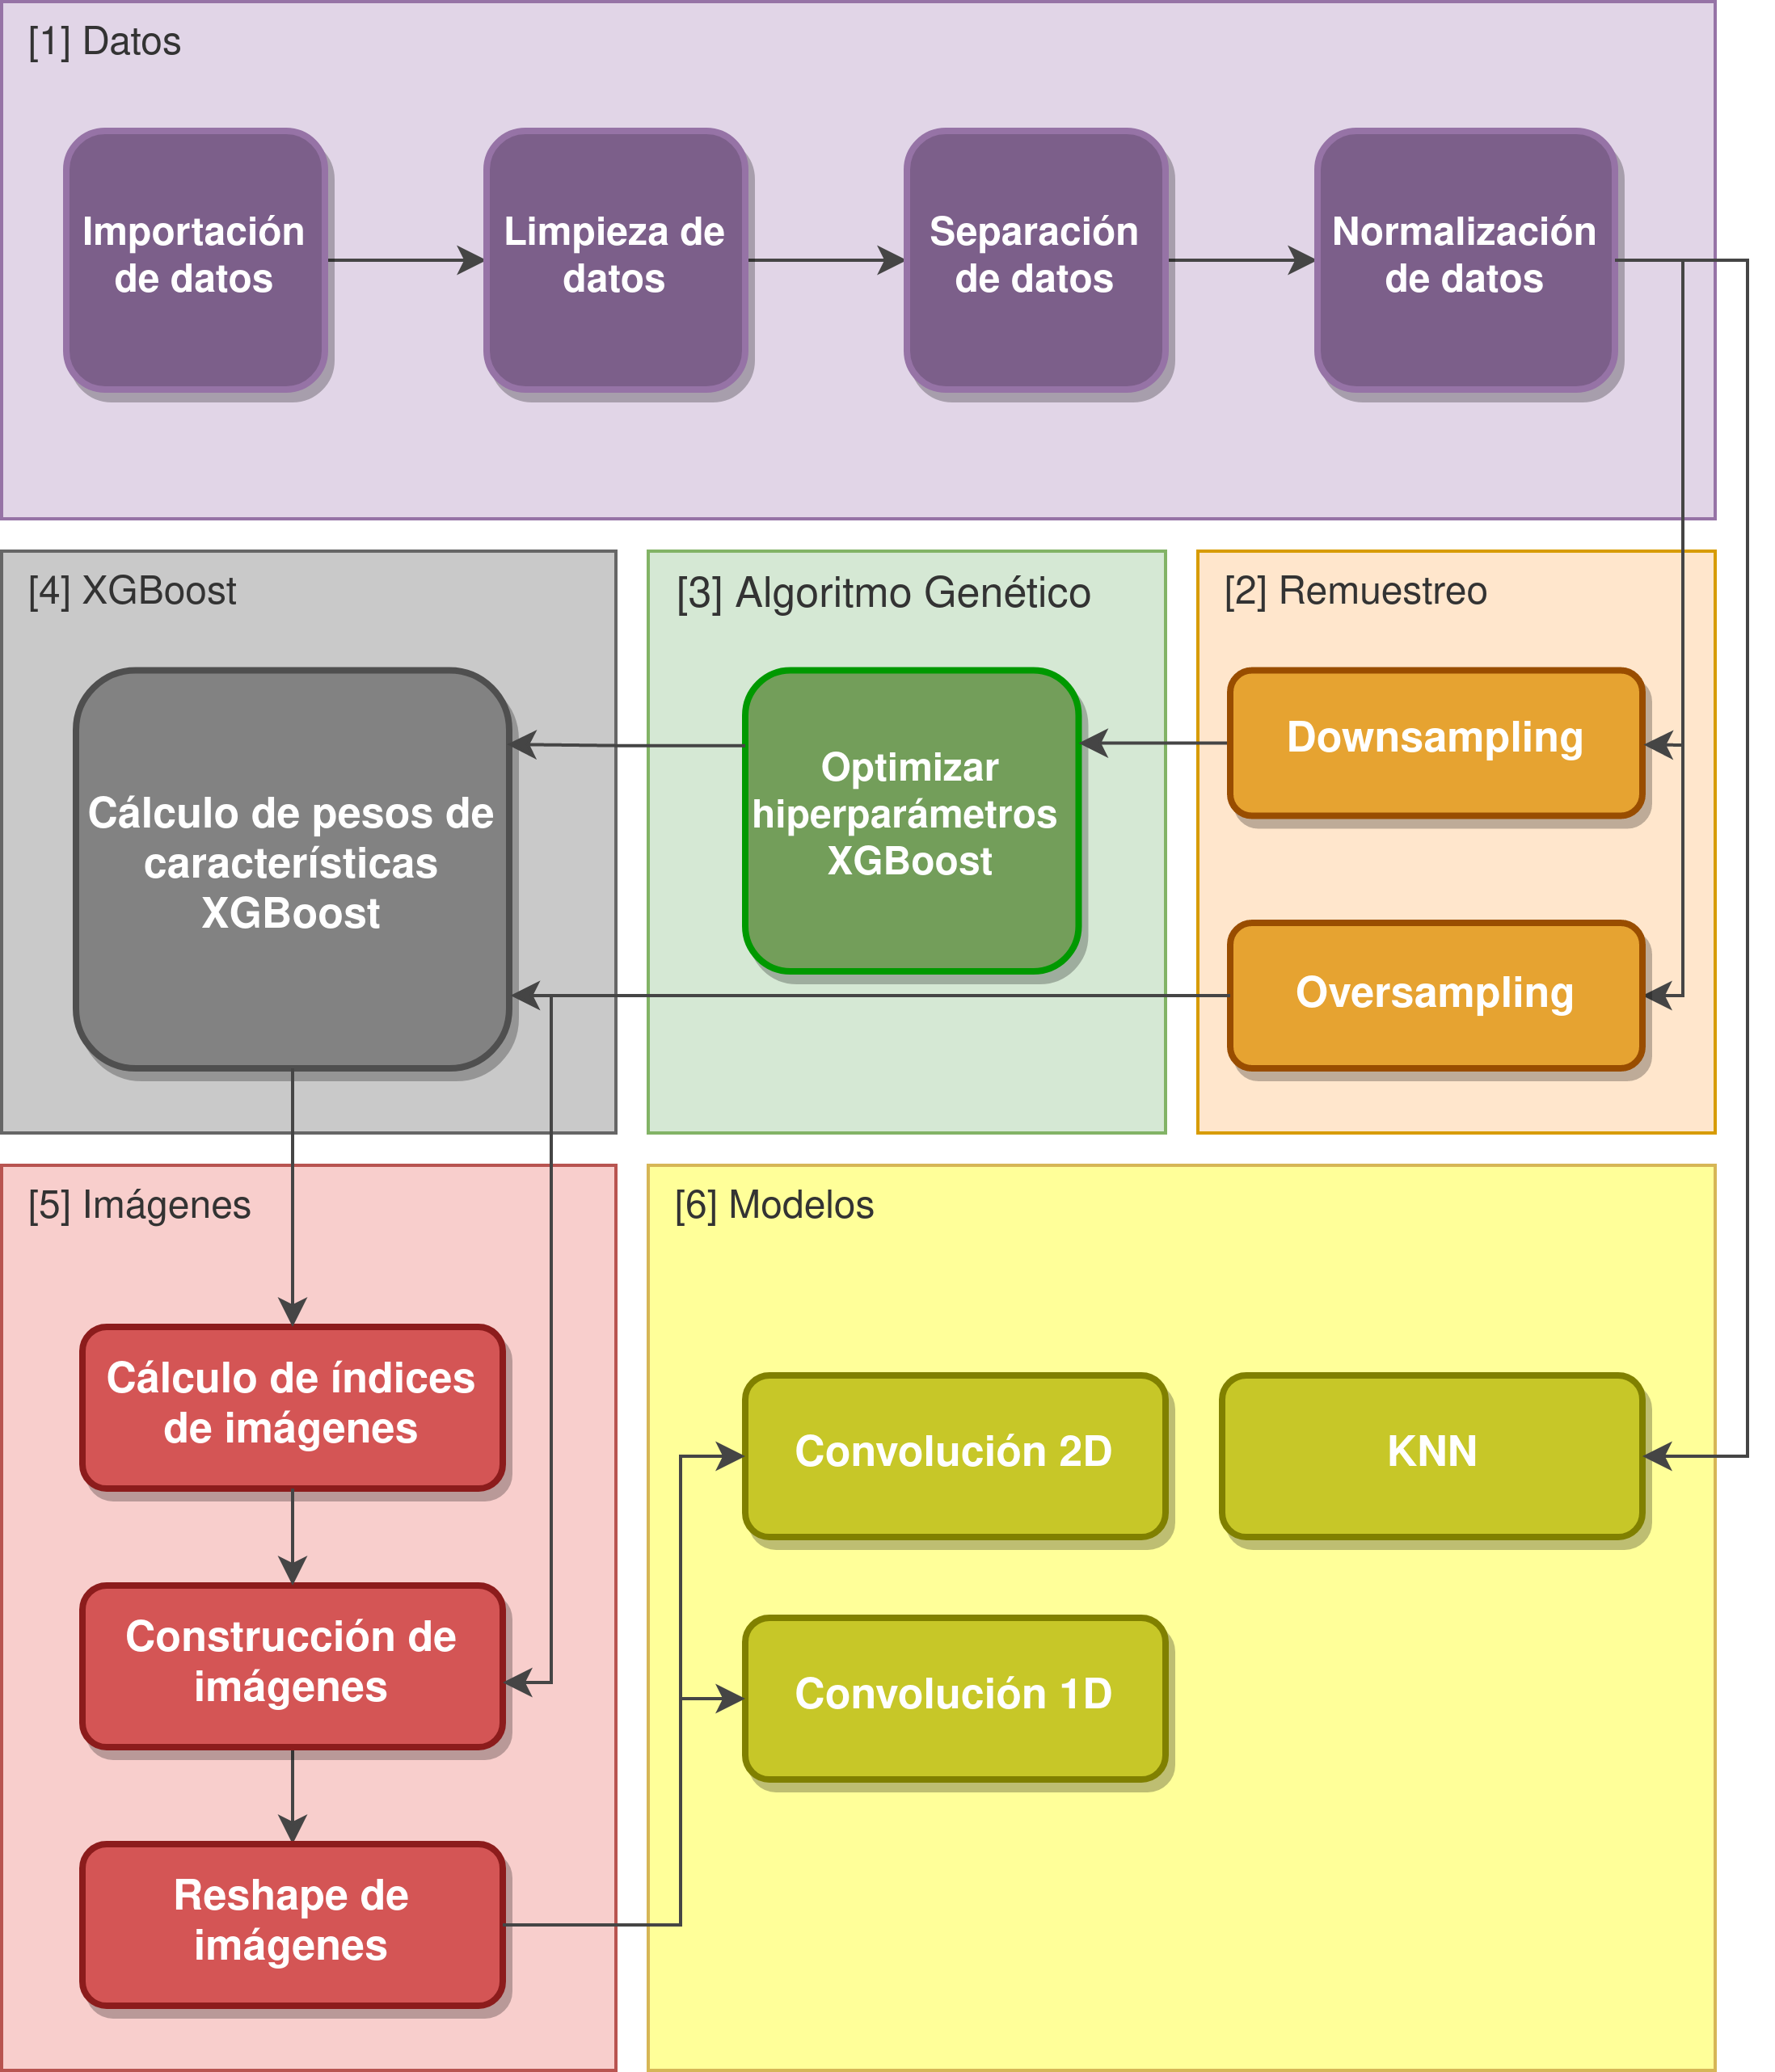
\includegraphics[width=15cm]{archivos/4.Metodologia/DataflowImageESP}
        \caption{Flujo de datos del proceso del proyecto.}
        \label{DataflowImage}
    \end{figure}


\section{Proceso}



    \subsection{Datos}


            Como en cualquier proyecto de \textit{Ciencia de Datos} el primer paso contempla la obtención, preparación y estudio de los datos. Este es el proceso en el que más tiempo se invierte en el ciclo de vida de un proyecto, algunos estudios apuntan que alrededor del 80 por ciento del tiempo en un proyecto se destina a esta tarea \cite{LifecycleDataScienceProjectsTimes}, por lo que es extremadamente importante aplicar buenas prácticas a la hora de llevar a cabo esta fase.

            El conjunto de datos con el que se ha trabajado en este proyecto describe accidentes de tráfico de la ciudad de Madrid en un periodo concreto, desde el año 2019 hasta el 2022. Este dataset ha sido obtenido desde la web \cite{DatasetMadrid}, repositorio donde es posible encontrar distintos datasets relativos a la Comunidad de Madrid.

            El número total de registros en este periodo de tiempo es de 60.966 instancias, cada una de las cuales consta de 17 características que se describirán en la tabla \ref{DescripcionDatosTabla}:

            \renewcommand{\arraystretch}{1.5}
            \begin{table}[H]
                \centering
                \begin{tabular}{|c|L{0.7\textwidth}|}
                    \hline
                    \textbf{Atributo}&\textbf{Descripción}\\
                    \hline
                    \texttt Número de expediente &
                    Identificador del incidente, si varios registros tienen el mismo número de expediente se consideran como un mismo accidente y cada registro representa cada una de las distintas personas involucradas en él (Conductor, Pasajero o Peatón).\\
                    
                    \hline
                    \texttt Fecha &
                    Día mes y año en el que se ha producido el incidente.\\
                    
                    \hline
                    \texttt Hora &
                    Hora y minuto del día.\\

                    \hline
                    \texttt Localización &
                    Nombre de la calle (si procede).\\

                    \hline
                    \texttt Número &
                    Número de la calle donde ha ocurrido el incidiente (si procede).\\

                    \hline
                    \texttt Distrito &
                    Nombre del distrito de Madrid donde ha ocurrido el incidente.\\

                    \hline
                    \texttt Tipo de accidente &
                    Tipología de accidente, puede ser de diversos tipos (Colisión doble, Colisión múltiple, Alcance, Choque contra obstáculo, Atropello, Vuelco, Caída, Otras causas).\\

                    \hline
                    \texttt Estado meteorológico &
                    Condiciones climatológicas en el momento del incidente (Despejado, Nublado, Lluvia débil, Lluvia intensa, Granizado o Nevando)\\

                    \hline
                    \texttt Tipo de vehículo &
                    Clasificación en función del tipo de vehículos, p.e. motocicleta, turismo, cuadriciclo, etc.\\

                    \hline
                    \texttt Tipo de persona &
                    Rol de la persona involucrada (Conductor, Pasajero o Peatón)\\

                    \hline
                    \texttt Rango de edad &
                    Intervalo de edad la persona implicada.\\

                    \hline
                    \texttt Sexo &
                    Sexo de la persona implicada (Hombre o Mujer).\\

                    \hline
                    \texttt Lesividad &
                    Consecuencias físicas de la persona implicada, si ha necesitado asistencia sanitaria, si ha sido ingresada o si ha sido mortal.\\

                    \hline
                    \texttt Coordenada X &
                    Coordenada X del accidente en formato \textit{UTM}.\\

                    \hline
                    \texttt Coordenada Y &
                    Coordenada Y del accidente en formato \textit{UTM}.\\

                    \hline
                    \texttt Positivo en alcohol &
                    Si la persona implicada ha dado positivo en el control de alcoholemia (S o N).\\

                    \hline
                    \texttt Positivo en drogas &
                    Si la persona implicada ha dado positivo en el control de estupefacientes (S o N).\\

                    \hline
                \end{tabular}
                \caption{Descripción de los datos.}
                \label{DescripcionDatosTabla}

            \end{table}


            Hay que resaltar la importancia del atributo lesividad, puesto que es la variable respuesta de este trabajo. Existen una serie de valores asignados a esta categoría, así cada cdato de lesividad pertenece, al menos, a uno de los siguientes casos:

              \begin{itemize}
                    \item Consecuencias leves: comprende desde aquellas personas que no han resultado heridas hasta aquellas que han necesitado ingresar en un centro hospitalario no más de 24 horas. El tipado numérico de estas casuísticas es el siguiente:

                        \begin{itemize}
                            \item 1: Atención en urgencias sin posterior ingreso.
                            \item 2: Ingreso inferior o igual a 24 horas.
                            \item 5: Asistencia sanitaria ambulatoria con posterioridad.
                            \item 7: Asistencia sanitaria sólo en el lugar del accidente.
                            \item 14: Sin asistencia sanitaria.
                        \end{itemize}

                    \item Consecuencias severas: implicados que han requerido un ingreso hospitalario superior a 24 horas. En este caso el tipado numérico del conjunto de datos corresponde a:

                        \begin{itemize}
                            \item 3: Ingreso superior a 24 horas.
                        \end{itemize}

                    \item Consecuencias fatales: víctimas mortales dentro del margen de las 24 horas posteriores al accidente. La asignación numérica a este campo es:

                        \begin{itemize}
                            \item 4: Fallecido 24 horas.
                        \end{itemize}

                \end{itemize}


            Se pueden consultar más detalles de las características del dataset descripción del conjunto de datos del portal \textit{Open Data} de Madrid \cite{InfoDatasetMadrid}.


            \begin{enumerate}

                \item \textbf{Limpieza de datos}

                    Una vez importados los datos, es indisepensable hacer una limpieza de éstos (\textit{Data Cleaning}), eligiendo las características que serán utilizadas como variables explicativas en las predicciones atendiendo además a los valores de las instancias, ya que pueden contener valores nulos, valores atípicos (\textit{outliers}) o contener valores erróneos. Esta problemática requiere de la aplicación de distintas fases de análisis.

                    En el caso del dataset de accidentes de tráfico de este proyecto se han escogido las siguientes características como variables explicativas: \textit{hora, distrito, tipo accidente, estado meteorológico, tipo vehiculo, tipo persona, rango edad, sexo, positivo alcohol, positivo drogas, vehiculos implicados, coordenada x utm, coordenada y utm}.


                    Una vez que se han obtenido las variables (también denominados predictores) con los que trabajarán los modelos, se han eliminado aquellos registros duplicados y aquellos que tuvieran algún valor. Por lo tanto, las dimensiones finales del conjunto de datos pasarán a ser 12 variables y 54.364 registros con respecto a las 17 características y 60.966 filas originales. 

                \item \textbf{Transformaciones de datos}

                    A continuación se requiere la realización de transformaciones sobre los datos para que los modelos utilizados trabajen con un conjunto de datos bien definido y consistente. Gran parte de los modelos de \glsentryshort{ml} necesitan de datos de entrada numéricos para poder comprenderlos, además existe la necesidad de normalizar estos valores para que estén en la misma escala y el entrenamiento sea exitoso, por lo tanto, lo primero es la realización de una serie de transformacíones que conviertan las variables categóricas a variables numéricas.

                    En primer lugar ha sido necesario transformar las columnas \textit{coordenada x utm} y \textit{coordenada y utm} a números enteros, ya que estas variables eran inicialmente de tipo \textit{String}. Además, se da el caso de que el rango de estas variables es del orden de 7 a 10 dígitos, evitando cualquier formato de decimales estandarizado (utilizando puntos y comas indistintamente en distintas posiciones de los mismos), debido a esto ha sido necesario crear un proceso que analizase cada casuístca y los tradujese a un formato estandarizado.

                    Las columnas \textit{positiva alcohol} y \textit{positiva drogas} se han unido en una nueva columna debido a la cantidad de valores nulos que existía en la segunda variable, por lo que se crea una nueva columna que hace referencia a la intoxicacion etílica o de estupefacientes.
  

                    La variable \textit{localización} ha sido transformada a \textit{tipo de carretera}, con el objetivo de definir un criterio para clasificar el tipo de vía donde se ha producido el incidente, como por ejemplo una carretera, una autovía, glorieta, etc. Al no existir un servicio que ofrezca la tipología de la calle dado el nombre de la vía o las coordenadas, ha sido necesario tratar esta problema desde otro punto de vista mediante expresiones regulares. El término \textit{expresión regular} debe su origen a la teoría de las matemáticas y ciencias de computación, reflejan la propiedad de \textit{regularidad} que caracterizan a las expresiones matemáticas \cite{RegeXBook}. Una expresión regular es un tipo de patrón utilizado para encontrar una combinación de caracteres en una cadena de texto. Para clasificar el tipo de carreteras en este proyecto se han diseñado una serie de expresiones regulares que coinciden con ciertos criterios respecto a los valores de la variable \textit{localizacion} con el fin de distinguir distintos tipos de vía.


                    \textbf{NOTA: Ponemos una tabla con todas las RegEx que se han utilizado? Es sin duda la peor parte y menos científica del proyecto, y es lo único que no me gustaría mostrar, aunque ha llevado mucho tiempo me daría un poco de vergüenza poner esto en un proyecto de Ciencia de datos la verdad}


                    Las tipologías de clases de carreteras son \textit{Parking, Aeropuerto, Cuesta, Paseo, Parque, Túnel, Polígono, Camino, Glorieta, Puerta, Puente, Plaza, Bulevar, Travesía, Calzada, Carretera, Avenida, Autovía} y \textit{Calle}


                    No obstante, la aplicación de las expresiones regulares generalmente no son una solución empírica a un problema, ya que hay casos que pueden ser no contemplarse al diseñar estos patrones manualmente. En el caso de este proyecto su aplicación conlleva una serie de inconvenientes. Aśí, debido a las necesidades del problema, estas expresiones regulares están diseñadas jerárquicamente, de forma que aquellos valores de la variable \textit{localizacion} que coincidan con el primer patrón definido de la expresión regular serán asignados a esta categoría. Esto supone un impedimento a tener en cuenta, ya que muchos de los accidentes se producen en intersecciones, carriles de aceleración que conectan dos vías, vías cuyo nombre contiene el tipo de otra vía, etc. Por ejemplo si se da el caso de que exista algún patrón no definido como expresión regular, esto provocará que estas localizaciones se asignen con respecto al primer patrón definido encontrado, llegando a clasificar erróneamente el tipo de vía. Como consecuencia, la jerarquía de la definición de las expresiones regulares es un punto crítico ya que se busca maximizar la clasificación de aquellos tipos de vía con menor número de apariciones, como es el caso de parking o aeropuerto, mientras se minimiza el error en la clasificación.


                    Para solucionar esto, existen herramientas como Open Refine \cite{OpenRefine} que utilizan técnicas de clustering nominal para detectar semejanzas entre caracteres. Debido a las limitaciones de tiempo, esta técnica no se ha podido aplicar, aunque se propone como trabajos para futuro con el objetivo de aumentar el rendimiento de los modelos aplicados.

                    Por otro lado hay que tratar aquellos valores que no hayan coincidido con los patrones definidos (TODO: poner el número), sin embargo, al ser una cantidad de registros se han podido revisar manualmente coincidiendo todas con nombres de calles al que no se les ha asignado la palabra \textit{"calle"}.

                    En la variable \textit{hora}, al ser un campo continuo, ha sido necesario discretizarla según intervalos, distinguiendo entre noche y día en función de la hora en la que se ha producido el incidente.


                    En la tabla \ref{TransformacionDatosTabla} se define el resto de codificaciones aplicadas sobre el resto de variables del modelo para transformar estos campos a formato numérico.

                    \def\arraystretch{1.2}%
                    \begin{longtable}{|c|L{0.7\textwidth}|}\\

                        \hline
                        \textbf{Característica} & \textbf{Tipado}\\

                        \hline
                        \multirow{3}{*}{Lesividad}              & 0: Accidentes leves (\textit{1, 2, 5, 6, 7, 14}).\\
                                                                & 1: Accidentes severos (\textit{3}).\\
                                                                & 2: Accidentes fatales (\textit{4}).\\

                        \hline
                        \multirow{2}{*}{Hora}                   & 1: Noche (\textit{6 PM - 6 AM}).\\
                                                                & 2: Día (\textit{6 AM - 6 PM}).\\
                        \hline
                        \multirow{1}{*}{Distrito}               & Numeración en función de orden de aparición.\\

                        \hline
                        \multirow{2}{*}{Tipo Accidente}         & 1: Colisión fronto-lateral. \\
                                                                & 2: Alcance.\\
                                                                & 3: Colisión lateral.\\
                                                                & 4: Choque contra obstáculo fijo.\\
                                                                & 5: Colisión múltiple.\\
                                                                & 6: Caída.\\
                                                                & 7: Atropello a persona.\\
                                                                & 8: Colisión frontal.\\
                                                                & 9: Otro.\\
                                                                & 10: Solo salida de la vía.\\
                                                                & 11: Vuelco.\\
                                                                & 12: Atropello a animal.\\
                                                                & 13: Despeñamiento.\\
                        \hline
                        \multirow{7}{*}{Estado Meteorológico}   & 1: Despejado.\\
                                                                & 2: Nublado.\\
                                                                & 3: Lluvia débil.\\
                                                                & 4: Lluvia intensa.\\
                                                                & 5: Granizando.\\
                                                                & 6: Nevando.\\
                                                                & 7: Se desconoce.\\
                        \hline
                        \multirow{1}{*}{Tipo Vehículo}          & Numeración en función de orden de aparición.\\

                        \hline
                        \multirow{3}{*}{Tipo Persona}           & 1: Conductor.\\
                                                                & 2: Pasajero.\\
                                                                & 3: Peatón.\\
                        \hline
                        \multirow{5}{*}{Rango Edad}             & 1: Menores de 18 años.\\
                                                                & 2: De 18 a 25 años.\\
                                                                & 3: De 25 a 65 años.\\
                                                                & 4: Mayores de 65 años.\\
                                                                & 5: Edad desconocida.\\
                        \hline
                        \multirow{3}{*}{Sexo}                   & 1: Hombre.\\
                                                                & 2: Mujer.\\
                                                                & 3: Desconocido.\\
                        \hline
                        \multirow{2}{*}{Positivo}               & 1: Sí.\\
                                                                & 2: No.\\
                        \hline

                    \caption{Transformaciones aplicadas a los datos.}
                    \label{TransformacionDatosTabla}\\
                    \end{longtable}

                La transformación numérica de los datos es un proceso crítico, ya esta codificación será la entrada de los modelos utilizados. Una representación que no refleje correctamente el tipo de cada campo original influirá negativamente en la precisión de los modelos implementados.

                \item Análisis de datos

                    Una de las fases más importantes antes de comenzar el modelado en cualquier proyecto \textit{Data Science} es el análisis de datos. Este proceso tiene como objetivo la descripción de los datos, identificación de \textit{outliers}, valores erróneos y tendencias que se puedan dar en ellos.\\

                    Si se analizan los datos que correspondan a cada una de las tres posibles clases de lesividad (leves, severos y fatales) realizando un histograma \ref{OriginalDataHistogramImage}, se puede observar que el dataset se encuentra claramente desbalanceado con respecto a la variable respuesta, contando con 53.009 accidentes leves, 1.271 severos y 84 fatales.\\

                    Un conjunto de datos desbalanceado se define como aquel que contiene un número de instancias mucho mayor de determinadas clases con respecto al resto \cite{WhyImbalancedDataIsAProblem}. Esto se convierte en un problema para los modelos de clasificación ya que estos modelos tenderán a predecir las muestras como aquellas que pertenecen a las mayoritarias sobre el conjunto de test debido a que las reglas de clasificación de las clases menos numerosas tienden a ser ignoradas.

                    El desbalanceo de datos es un problema ampliamente estudiado a lo largo de los años y existen numerosos métodos orientados a solventarlo mediante distintas técnicas de muestreo \cite{ImbalancedDataReview}, por lo que será necesario remuestrear estos datos mediante la técnica \glsentryfull{smoteii}.


                    \begin{figure}[H]
                        \centering
                        \includesvg[scale=0.3]{archivos/4.Metodologia/Datos/Analisis/OriginalDataHistogram}
                        \caption{Histograma de clases de accidente en el conjunto de datos original.}
                        \label{OriginalDataHistogramImage}
                     \end{figure}

                    Es interesante observar el grado de correlación entre las variables de forma que si se encuentran campos muy correlacionados se podría eliminar alguno de ellos. Para realizar este análisis se utiliza el coeficiente de correlación de \textit{Pearson} \cite{PearsonCoefficientCorrelationMatrix}, que toma un rango de valores entre -1 y 1. Como resultado la correlación será más pronunciada cuanto más se aproxime a -1 o a 1 mientras que será más débil al aproximarse a 0.

                    En la figura \ref{CorrelationMatrixImage} podemos observar la matriz de correlación de las variables explicativas del conjunto de datos del proyecto. Analizando dicha matriz se puede comprobar que las únicas variables que están medianamente correlacionadas son \textit{coordenada x utm} y \textit{distrito}, con una correlación positiva de 0.44, sin embargo no es un valor tan alto como para eliminar alguna de las dos las características. Así pues, el estudio de la correlación muestra que las variables de datos elegidas no están correlacionadas y se puede continuar con la siguiente fase del proyecto.

                    \begin{figure}[H]
                        \centering
                        \includesvg[scale=0.3]{archivos/4.Metodologia/Datos/Analisis/CorrelationMatrix}
                        \caption{Matriz de correlación para los predictores escogidos del dataset.}
                        \label{CorrelationMatrixImage}
                     \end{figure}


                \item Normalización de datos

                    La normalización de datos es un proceso necesario a la hora de obtener buenos resultados en los modelos predictivos de \glsentryshort{ml}. Cuando un modelo es entrenado, existen características representadas en distintas escalas, y las que contienen un rango de valores numérico más alto, ya sea por la naturaleza de la variable o porque se encuentren en otro rango, dominan a las que se encuentren en un rango menor, influenciando negativamente en los modelos \glsentryshort{ml}, como por ejemplo las \glsentryshort{cnn} o \glsentryshort{knn} \cite{NormalizationSensitiveModels}.\\

                    Así pues, el proceso de normalización tiene como objetivo minimizar el sesgo de aquellas características cuya contribución sea mayor a la hora de encontrar patrones entre los datos. Existen distintas técnicas de normalización como por ejemplo \glsentryfull{mc}, \glsentryfull{vss} o \glsentryfull{mmn} entre otras [\cite{DataNormalizationInvestigation}].\\


                    En este proyecto se ha utilizado la normalización \glsentryfull{zsn} debido a que consigue representaciones de acuerdo a una distribución normal. Para ello, se utiliza la media y la desviación típica para reescalar los datos de tal forma que la distribución de ellos esté definida por una media de cero y una desviación típica unitaria.\\

                   \begin{center}
                        $x^* = \frac{x - u}{\sigma}$
                    \end{center}


                    Donde $x^*$ es una muestra de una característica de los datos, $u$ es la media total de dicha característica y $\sigma$ es la desviación típica total de los valores de la característica.

                    Los resultados obtenidos después de aplicar esta técnica se pueden interpretar como la distancia de cada valor con respecto a la media.

                \item Separación de datos

                    La siguiente fase en cualquier modelo de \glsentryshort{ml} es la separación de datos (\textit{split}). Esta fase consiste en dividir el conjunto total de registros en al menos dos subconjuntos, uno de entrenamiento y otro de test. El modelo se entrenará en base al conjunto de entrenamiento y se evaluará con el de test, los resultados sobre este conjunto permitirán comparar los modelos en base a las predicciones sobre las muestras que nunca han visto.\\


                    Comúnmente la proporción de datos de entrenamiento y test está establecida en \textit{0.8} y \textit{0.2} respectivamente, y  en nuestro caso hemos elegido un valor de \textbf{TODO: X por ciento} para el entrenamiento y el resto para el conjunto de test.


                    \begin{figure}[h]
                        \centering
                        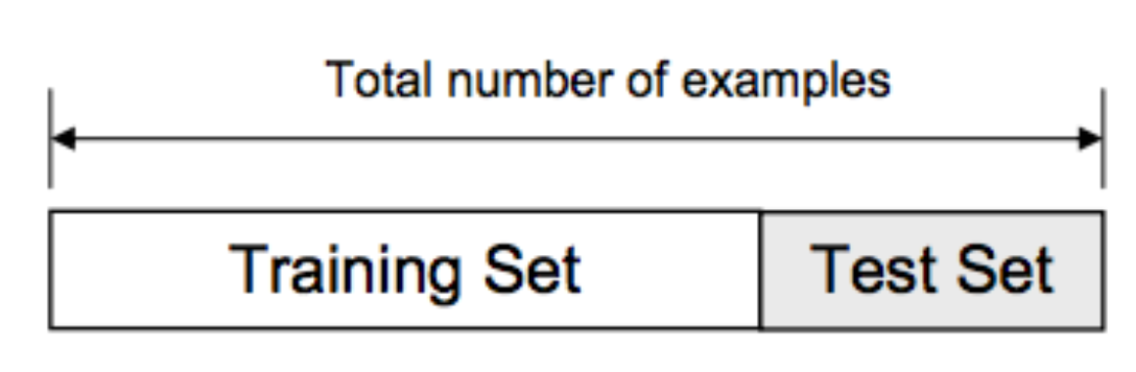
\includegraphics[width=7cm]{archivos/4.Metodologia/Datos/Separacion/DataSplit}
                        \caption{https://towardsdatascience.com/train-test-split-and-cross-validation-in-python-80b61beca4b6. División de un conjunto de datos en datos de entrenamiento y test.}
                        \label{DataSplitImage}
                     \end{figure}

            \end{enumerate}



        \subsection{Remuestreo}


            Con el objetivo de que el modelo no se vea muy afectado debido a la diferencia de las clases mayoritarias respecto a las minoritarias se hace necesaria la utilización de técnicas de remuestreo. Estas técnicas permiten operar sobre un conjunto de datos para balancearlos, y se aplican únicamente al conjunto de entrenamiento, ya que la intención  es influir sobre el aprendizaje del modelo para aumentar el rendimiento de las predicciones sobre el conjunto de test, si aplicásemos remuestreo sobre este último conjunto estaríamos falseando los resultados de las predicciones.


            En este proyecto se han hecho uso de las siguientes técnicas de remuestreo:

            
            \begin{enumerate}



                \item Downsampling: tiene como objetivo balancear el conjunto de datos para que todas las clases tengan el mismo número de muestras. Para ello se iguala el número de muestras de las clases mayoritarias a aquellas clases que contienen menos muestras, descartando aquellas que sobrepasen este límite \cite{Downsampling}. \textbf{NOTA: Aún no se sabe si se va a aplicar Downsampling o no, sigo con los experimentos, de momento lo dejaré así a la espera de ver más resultados, queda pendiente para revisión}
                

                \item Generación de datos sintéticos: técnica que permite generar datos artificiales en base a los límites que separan unas clases de otras. Se ha hecho uso de la tećnica \glsentryfull{smoteii} \cite{SMOTEII}. Esta técnica selecciona los vecinos más cercanos de la misma clase y genera nuevas muestras en base al espacio entre la clase minoritaria y sus vecinos más cercanos.\\

                \glsentryshort{smoteii} ha sido utilizado para generar más muestras artificiales de los accidentes pertenecientes a las clases minoritarias (\textit{severos} y \textit{graves}). Este nuevo conjunto de datos servirá como entrenamiento para los modelos, evitando que tiendan al sobreajuste. En la figura \ref{SMOTEIIDataHistogramImage} se aprecia el histograma tras haber aplicado \glsentryshort{smoteii}, contando ahora con 42508 muestras de cada una de las clases de accidentes.
    
            \end{enumerate}


            Una vez aplicadas las técnicas de remuestreo, es útil observar cuál es la representación espacial de los datos sintéticos generados por \glsentryshort{smoteii} en deferencia a los datos originales mediante el método \glsentryfull{tsne} \cite{TSNEPaper}. \glsentryshort{tsne} es un algoritmo que permite visualizar las proyecciones de datos multidimensionales en espacios bidimensionales o tridimensionales. Este modelo debe su origen a su antecesor \glsentryfull{sne}, siendo una versión optmizada de éste.

            Mientras que \glsentryshort{sne} proyecta los datos convirtiendo las distancias Euclídeas entre las muestras a probabilidades condicionales, el \glsentryshort{tsne} modifica la función de coste para proyectarlos mediante una distribución t-Student, permitiendo además trabajar con gradientes simplificados.


            En la figura \ref{TSNEImages} se muestran las proyecciones de \glsentryshort{tsne} (tanto la representación bidimensional como la tridimensional) sobre el conjunto de datos de entrenamiento original y aquellos que han sido generados artificialmente por \glsentryshort{smoteii}.

            El \glsentryshort{tsne} de 2D aplicado sobre los datos generados por \glsentryshort{smoteii} \ref{TSNEImages:Train2D} nos permite observar cómo se han generado las muestras con respecto a los datos originales \ref{TSNEImages:Clean2D} en una proyección bidimensional. Se aprecia cómo se han producido las nuevas muestras de los accidentes graves (azul) calculando la cercanía de los puntos en base a las fronteras de división. \textbf{Nota: Realmente yo no veo nada}.


            \begin{figure}
                \centering
                \begin{subfigure}[b]{0.4\textwidth}
                    \centering
                    \includesvg[scale=0.4]{archivos/4.Metodologia/Datos/Resampling/TSNE/2d_tsne_clean}
                    \caption{TSNE de 2 componentes aplicado a los datos originales.}
                    \label{TSNEImages:Clean2D}
                \end{subfigure}
                % Añadir el espacio deseado, si se deja la linea en blanco la siguiente subfigura ira en una nueva linea
                \begin{subfigure}[b]{0.4\textwidth}
                    \centering
                    \includesvg[scale=0.4]{archivos/4.Metodologia/Datos/Resampling/TSNE/2d_tsne_train}
                    \caption{TSNE de 2 componentes aplicado a los datos generados por SMOTE-II.}
                    \label{TSNEImages:Train2D}

                \end{subfigure}
                \begin{subfigure}[b]{0.4\textwidth}
                    \centering
                    \includesvg[scale=0.4]{archivos/4.Metodologia/Datos/Resampling/TSNE/3d_tsne_clean}
                    \caption{TSNE de 3 componentes aplicado a los datos originales.}
                    \label{TSNEImages:Clean3D}
                \end{subfigure}
                \begin{subfigure}[b]{0.4\textwidth}
                    \centering
                    \includesvg[scale=0.4]{archivos/4.Metodologia/Datos/Resampling/TSNE/3d_tsne_train}
                    \caption{TSNE de 3 componentes aplicado a los datos generados por SMOTE-II.}
                    \label{TSNEImages:Train3D}
                \end{subfigure}
                \caption{TSNE de 2 y 3 componentes aplicado a los datos originales y a los generados sintéticamente (\glsentryshort{smoteii}).}
                \label{TSNEImages}
             \end{figure}



    \subsection{Algoritmo Genético}


        Para entrenar el modelo haremos uso del algoritmo \glsentryshort{xgboost}. Y para que este entrenamiento sea adecuado es importante optimizar los hiperparámetros del mismo.\\

        Para ello se ha hecho uso de algoritmos genéticos, donde cada individuo perteneciente a la población de una generación está formado por una configuración de hiperparámetros específica, de tal forma que a lo largo de las iteraciones los individuos evolucionarán mediante el cruce y la mutación para dar lugar a nuevas configuraciones de hiperparámetros optimizadas [\cite{GAXGBoostPaper}].

        Debido al coste computacional que tendría optimizar todos los parámetros por la magnitud del espacio de búsqueda y al no ser necesario tener en cuenta todos ellos, se ha seleccionado un subcojunto de aquellos que más influencia tienen en el entrenamiento del modelo. Estos hiperparámetros de los que consta cada individuo de la población son:

        \begin{enumerate}

            \item Profundidad máxima: es la máxima altura que puede tomar el árbol. Si el árbol de decisión alcanza demasiada profundidad tenderá al \textit{overfitting} ya que aprenderá relaciones complejas entre los datos que pueden deberse a ruido en los datos de entrenamiento.

            \item Peso mínimo de los hijos: es el mínimo peso que se establece a la hora de crear un nuevo nodo en el árbol. Cuando se entrena un árbol de decisión éste genera nuevos nodos en base a máxima separabilidad de los datos de entrenamiento en cada nivel. Con el límite de peso de los hijos establecemos un umbral mínimo de muestras que deben pertenecer a un nodo para realizar la separación. Un valor bajo en este parámetro permitirá crear nodos con menos muestras y por lo tanto el modelo tenderá al \textit{overfitting}.

            \item ETA: tamaño de paso utilizado para aplicar descenso por gradiente para minimizar la pérdida de los árboles anteriores.

        \end{enumerate}

        La inicialización y mutación de los valores de los individuos viene dada por una limitación mínima y máxima. Si esta restricción no se contemplase, los hiperparámetros podrían tomar valores extremos, reduciendo así el rendimiento de entrenamiento y el de las predicciones. Por lo tanto los individuos variarán sus parámetros tomando un valor aleatorio dentro de rangos definidos. Los parámetros de las nuevas soluciones mutarán dentro de unos límites específicos para cada parámetro establecidos como máximos y mínimos.

        \begin{table}[H]
            \centering
                \begin{tabular}{ |c|c|c| } 
                \hline
                \textbf{Hiperparámetro} & \textbf{Inicialización} & \textbf{Mutación}\\
                \hline
                    Profundidad Máxima & [1, 25] & [-6, 6]\\ 
                    Peso mínimo de los hijos & [0.01, 20.0] & [-7, 7] \\ 
                    ETA & [0.01, 1] &  [-0.3, 0.3] \\ 
                \hline

                \end{tabular}

            \caption{Límites de inicialización y mutación de los hiperparámetros de los individuos.}
            \label{InitAndMutationLimitsHyperparamsTable}
        \end{table}

        Una vez inicializados aleatoriamente los TODO:X individuos especificados en la población, éstos se evaluarán instanciando TODO:X modelos \glsentryshort{xgboost} con los valores de cada individuo en la población. El conjunto de datos sobre el que entrenará cada instancia \glsentryshort{xgboost} será el conjunto de entrenamiento TODO:XX. La función \textit{fitness} que evaluará cada individuo será la métrica TODO:F1-X aplicada sobre el conjunto de test obtenido en el proceso de separación de datos.

        \textbf{TODO: No se redactará más hasta tener claro cuál es la mejor forma de entrenar el \glsentryshort{xgboost} (función de validación y datos de entrenamiento)}





        %SE HACE CON EL CONJUNTO DE ENTRENAMIENTO DOWNSAMPLED
        %SE TESTA CON VALIDACION

    \subsection{XGBoost}


        \textbf{TODO: Decir si se entrena con downsampled o smote-ii en función de los experimentos cuando acabemos}\\

        Una vez se han optimizados los hiperparámetros del \glsentryshort{xgboost}, se entrena un nuevo modelo con los pq4m354ow calculados sobre el conjunto de entrenamiento remuestreado. Con este nuevo modelo \glsentryshort{xgboost} entrenado se obtiene la importancia de cada clase mediante la ponderación de sus pesos [\cite{XGBoostFeatureWeightsMeaning}]. Estos pesos son calculados por \glsentryshort{xgboost}, e indican el grado de importancia que ha tenido cada característica del conjunto de datos a la hora de entrenar el árbol, por lo tanto, aquellas caracerísticas a las que se les asigne más peso habrán sido aquellas que han jugado un papel clave en las decisiones de los árboles.

        Los pesos son asignados para cada característica del conjunto de datos con el que ha sido entrenado \glsentryshort{xgboost} de tal forma que permite realizar un análisis comparativo de los atributos y saber qué predictores son más importantes.


    \subsection{Matrices}


        Las \glsentryshort{cnn} aprenden patrones sobre la entrada de datos como matrices, esto implica que estén construidas de tal forma que se maximice la representación de la información, es decir, es necesario aplicar técnicas que posicionen cada característica en un elemento de la matriz maximizando la información de los accidentes (TODO: \textbf{relamente no entiendo muy bien la motivación que ha seguido la gente de TASPCNN a la hora de construir las imágenes, falta entender por qué lo hacen así, no lo he encontrado en el paper.})

        Por lo tanto, una vez se tienen los datos normalizados y muestreados, el siguiente paso será transferir cada una de las muestras tabulares de los accidentes a una matriz (\textit{5 x 5}), donde a cada característica se le asignará un elemento de la matriz, de tal forma que éstas sean la entrada a las \textit{CNN}.

        Para este objetivo se va a aplicar el algoritmo \textit{FV2GI} propuesto en el artículo [\cite{TASPCNN}], que asigna las características de una muestra en representación tabular en función de la importancia que éstas presenten en una jerarquía.

        Tal y como se propone en \cite{JerarquiaImagenes} las características que provocan un accidente de tráfico pueden englobarse en una serie de elementos o categorías principales, concretamente: \textit{características del conductor, el estado de la carretera, características propias del vehículo y condiciones del ambiente}. Basándonos en esto se realizará una asignación de cada característica del dataset en una de estas categorías. La tabla \ref{JerarquiaCaracteristicasTabla} muestra las asignaciones de las variables explicativas del conjunto de datos en función de esta jerarquía.


        \begin{table}[H]
          \centering
          \begin{tabular}{ |c|c| }
               \hline
               \textbf{Categoría} & \textbf{Variable}\\

               \hline
               \multirow{4}{*}{Accidente}            & Coordenada X.\\
                                                     & Coordenada Y.\\
                                                     & Hora.\\
                                                     & Vehículos implicados.\\
                                                     & Tipo de accidente.\\

               \hline
               \multirow{1}{*}{Ambiente}             & Estado meteorológico.\\

               \hline
               \multirow{2}{*}{Carretera}            & Tipo Carretera.\\
                                                     & Distrito.\\

               \hline
               \multirow{4}{*}{Conductor}            & Tipo Persona.\\
                                                     & Sexo.\\
                                                     & Rango Edad.\\
                                                     & Positivo.\\

               \hline
          \end{tabular}
          \caption{Transformaciones aplicadas a los datos.}
          \label{JerarquiaCaracteristicasTabla}
        \end{table}



        Una vez definida la jerarquía de características y los pesos asociados a cada una de ellas gracias al algoritmo \glsentryshort{xgboost}, se construyen las matrices de acuerdo al criterio \textit{FV2GI}. Este proceso consta de los siguientes pasos:

        \begin{enumerate}

            \item Generación de \textit{n} matrices inicializadas a 0, donde \textit{n} es el número de muestras tabulares en el dataset.
            \item Asignación de una fila a cada padre en función de su peso.
            \item Asignacíón de cada característica hija, en función de su peso, dentro de la fila de su padre.
        
        \end{enumerate}

        Se deben tomar las siguientes consideraciones a la hora de aplicar el algoritmo:

        \begin{enumerate}

            \item La importancia de un padre viene dada por ĺa suma de los pesos de las características hijas, en la tabla \ref{PesosFinalesCaracteristicas} se observa el cálculo de cada característica para las categorías principales.

            \item La asignación de las filas de la matriz a las características padres se realiza de forma intercalada en función de su peso. Aquel padre que más importancia tenga irá posicionado en la fila central de la matriz, el segundo padre irá posicionado por encima de éste y el tercero por debajo y así sucesivamente, de tal forma que se irá creando una estructura en la que dichos padres se interpolan entre las filas en función de su peso.

            \item Una vez se han asignado las categorías padre a las filas se realiza el mismo procedimiento con las características hijas a nivel de columna. Estas características se asignarán en una posición dentro de la fila de su categoría padre, donde aquella que más importancia tenga irá posicionada en el centro, la segunda irá posicionada a su izquierda, la tercera a la derecha y así sucesivamente.
        \end{enumerate}

        \textbf{Nota: No estoy contento con la explicación, creo que estaría bien meter una fórmula matemática o pseudocódigo y cambiar la redacción}


        \begin{figure}[H]
            \centering
            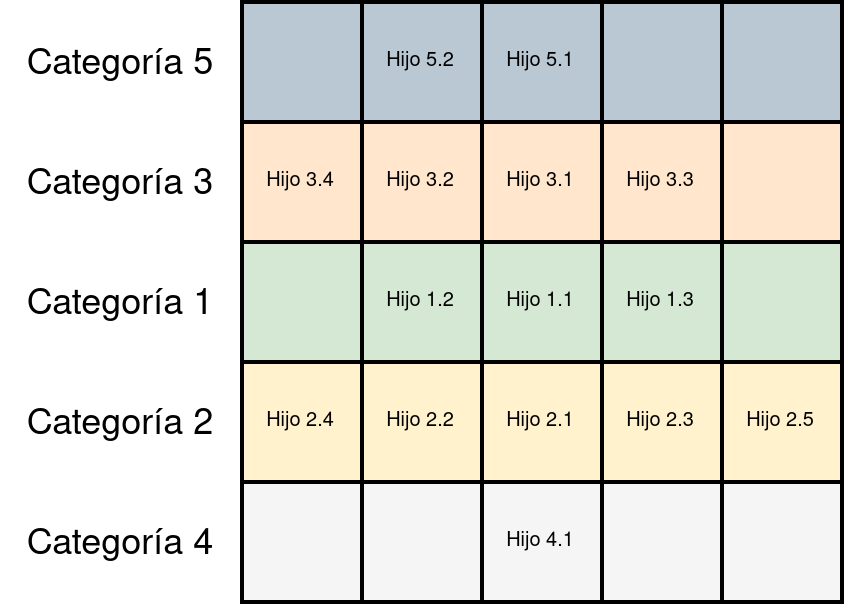
\includegraphics[width=7cm]{archivos/4.Metodologia/Matrices/FV2I}
            \caption{Ejemplo de posicionamiento de los elementos en una matriz. A las características se les asignan las filas en función de su peso y a las categorías hijas una columna dentro de la categoría correspondiente en función de su peso.}
            \label{FV2IExampleImage}
        \end{figure}

        Como resultado de este proceso se obtienen las matrices que serán la entrada de las \glsentryshort{cnn}.

        \begin{figure}[H]
            \centering
            \includesvg[scale=0.5]{archivos/4.Metodologia/Matrices/GrayImages/madrid_image_example_0}
            \includesvg[scale=0.5]{archivos/4.Metodologia/Matrices/GrayImages/madrid_image_example_1}
            \includesvg[scale=0.5]{archivos/4.Metodologia/Matrices/GrayImages/madrid_image_example_2}

            \caption{Representación de las muestras de accidentes en forma de matriz.}
            \label{SampledImagesExampleImage}
        \end{figure}

    \subsection{Modelos}


        En esta sección analizaremos los modelos utilizados en este proyecto para la realización de un estudio comparativo entre las arquitecturas.


        \begin{enumerate}

            \item KNN

                El método \glsentryshort{knn} servirá como referencia para testar el rendimiento del resto de modelos. Al ser un método que se aplica sobre un conjunto de datos tabular original, no hará uso de las matrices generadas.

                Es necesario optimizar los parámetros de este algoritmo para conseguir un buen rendimiento, por lo que aplicaremos la técnica \textit{Grid Search} \cite{GridSearchSklearnLibrary}. Esta técnica permite la optimización de los valores de los hiperparámetros mediante una búsqueda exhaustiva en un espacio de búsqueda definido por el usuario, probando distintas combinaciones hasta cubrirlo por completo. 

                \glsentryshort{knn} construirá el espacio de proyecciones mediante los datos de entrenamineto remuestreados por \glsentryshort{xgboost}, y clasificará las muestras del conjunto de test en base a la cercanía de los vecinos proyectados del conjunto de entrenamiento.


            \item CNN

                Una vez definidos los pasos que sigue el entrenamiento de una \textit{NN} y las características propias de las \textit{CNNs}, podemos analizar las arquitecturas de las \textit{CNNs} implementadas que se han aplicado en este proyecto. Cabe mencionar que el funcionamiento de ambas \textit{CNNs} únicamente difiere en el tamaño del \textit{kernel} (unidimensionales o bidimensionales según sea el caso correspondiente) y la forma en la que éste se desplaza debido a su dimensionalidad, por lo tanto detallaremos ambas arquitecturas de la misma forma.

                La arquitectura consta de cuatro capas convolucionales con tamaños de kernel (\textit{1 x 3}) en caso de las \glsentryshort{cnn1d} y de tamaño (\textit{3 x 3}) para las \glsentryshort{cnn2d}. Estos kernels se proyectarán en \textit{256} canales para formar el filtro convolucional asociado a cada capa. A la salida de cada uno de los mapas de características se aplica un proceso de \glsentryshort{batchnormalization}.

                El \textit{padding} del kernel se ha establecido en 1 para ambos tipos de redes, de tal forma que las convoluciones se aplicarán añadiendo ceros en los límites de las matrices, y los \textit{strides} en (\textit{1}) para las \glsentryshort{cnn1d} y (\textit{1, 1}) para las \glsentryshort{cnn2d}, por lo tanto el desplazamiento de los kernels se hará píxel a píxel tanto en las \glsentryshort{cnn1d} como en las \glsentryshort{cnn2d}.

                A la salida de cada capa convolucional se aplica la función de activación \glsentryfull{relu}, que se comporta devolviendo el valor $0$ para aquellas entradas que sean negativas y el valor original para aquellas que sean positivas, se puede apreciar el comportamiento en la figura \ref{RELUImage}. El rendimiento de esta función de activación en el campo de las imágenes está ampliamente extendido, además, evita la probabilidad de aparición del gradiente evanescente [\cite{GradientVanishingRelu}].

                \begin{center}
                    $f(x) = \left\{
                                   \begin{array}{lr}
                                     0 & \text{if } x<=0\\
                                     x & \text{if } x>0
                                   \end{array}
                            \right.$
                \end{center}

                \begin{figure}[h]
                    \centering
                    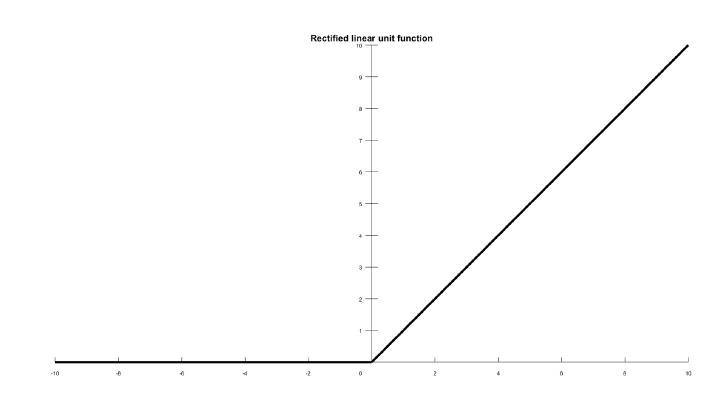
\includegraphics[width=10cm]{archivos/4.Metodologia/Modelos/CNN/RELUImage}
                    \caption{https://www.researchgate.net/journal/Transport-in-Porous-Media-1573-1634. Función ReLU}
                    \label{RELUImage}
                 \end{figure}

                La salida de la última capa de la convolución transformará el mapa de características de tamaño (\textit{5 x 5}) generada a una capa Flatten, que aplanará la matriz de tal forma que la convertirá en un vector unidimensional de (\textit{1 x 25}). A continuación se aplicará una capa densa que conectará cada uno de los \textit{25} nodos de la capa \textit{Flatten} con los \textit{128} nodos de la capa densa, que generará los logits antes de aplicar la última función de activación \textit{Softmax} que devolverá la clase predicha.


                Para ejemplificar la arquitectura de las \glsentryshort{cnn} propuestas se muestra el caso de la \glsentryshort{cnn2d} en la figura \ref{TASPCNNIMAGE}


                \begin{figure}[h]
                    \centering
                    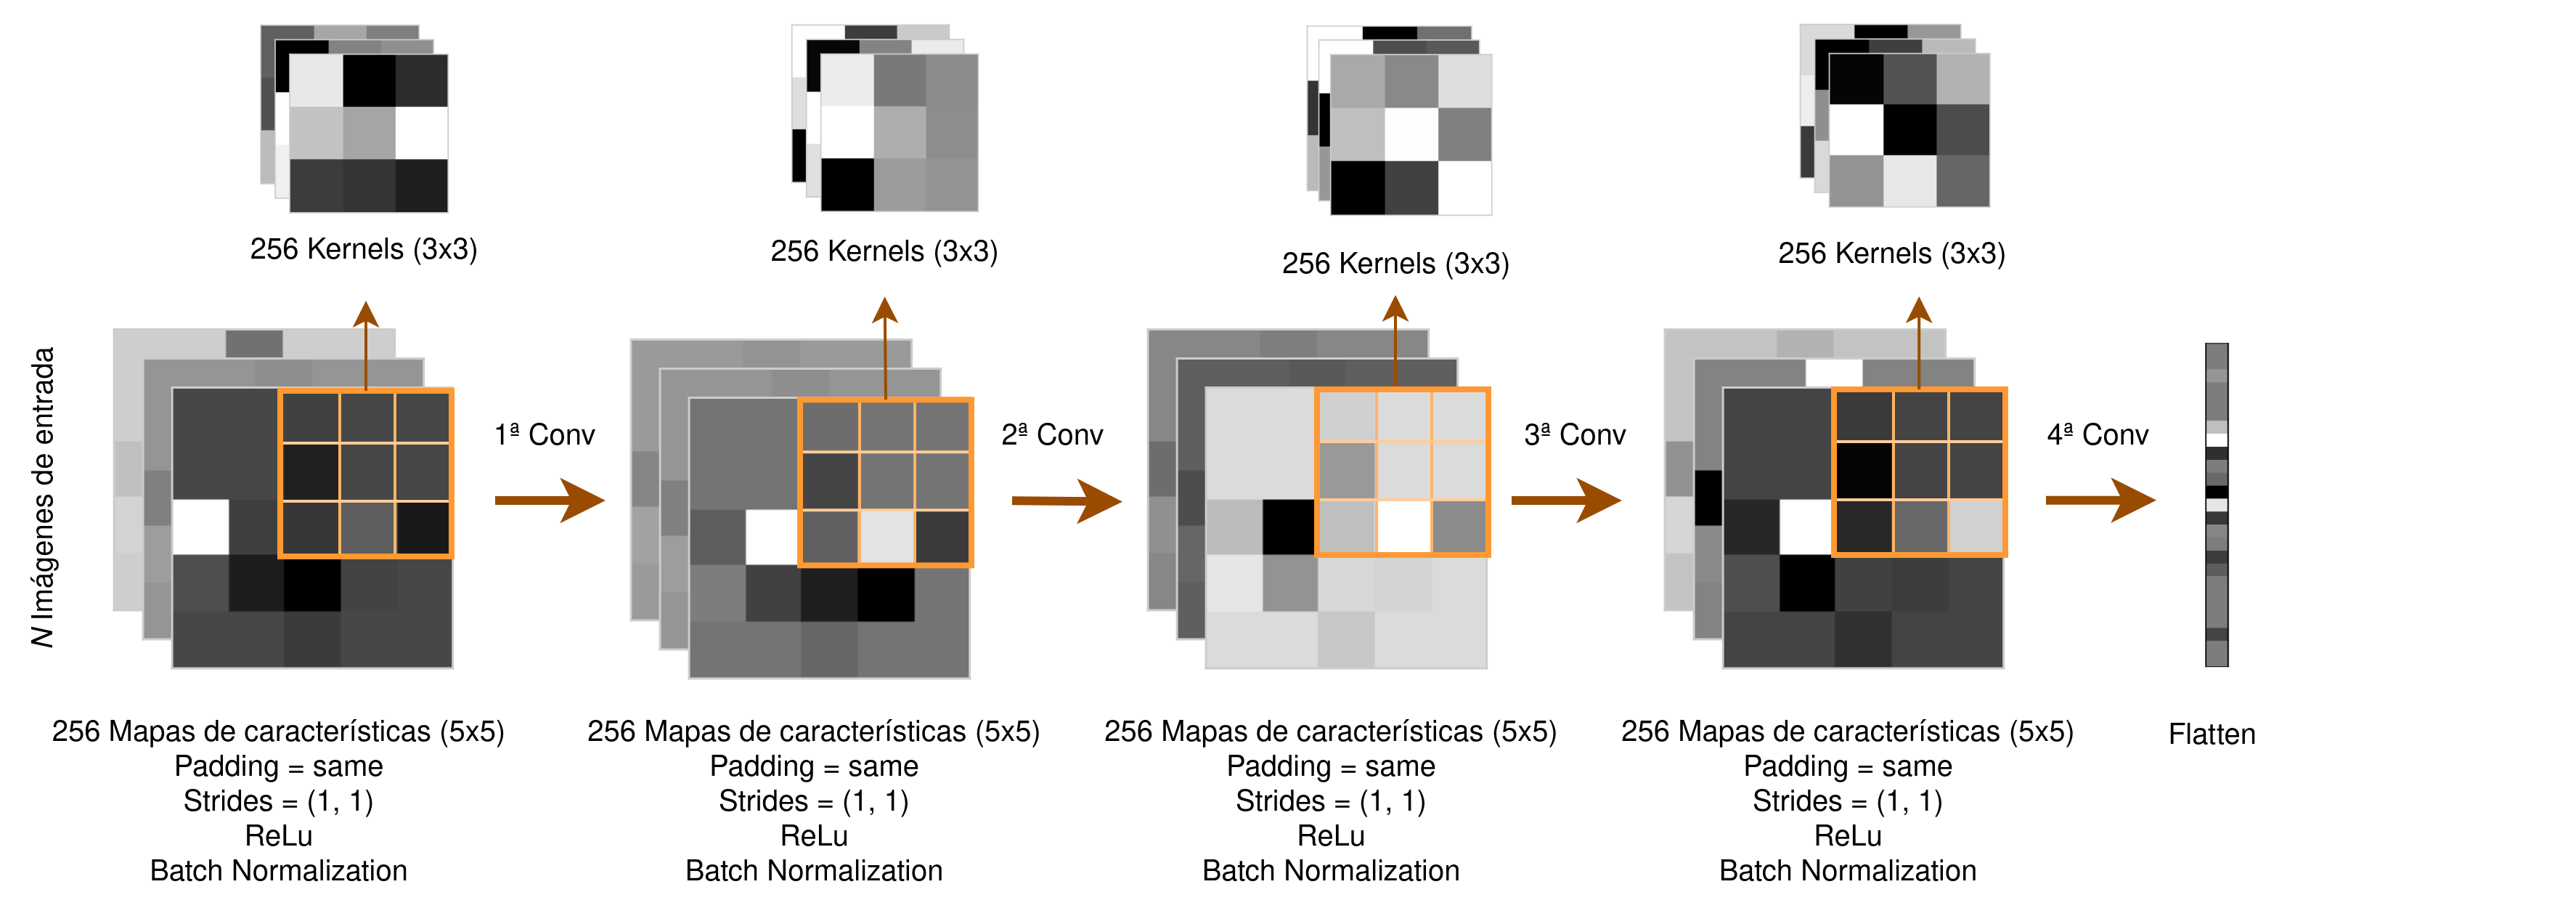
\includegraphics[width=17cm]{archivos/4.Metodologia/Modelos/CNN/2D/TASPCNN}
                    \caption{Arquitectura de la CNN-2D mostrando una  kernels aprendidos durante el entrenamiento.}
                    \label{TASPCNNIMAGE}
                 \end{figure}


        \end{enumerate}

        \cite{AutoSklearn}

\newpage
	% Plantilla: Se muestran figuras
%%%%%%%%%%%%%%%%%%%%%%%%%%%%%%%%%%%%%%%%%%%%%%%%%%%%%%%%%%%%%%%%%%%%%%%%
% Plantilla TFG/TFM
% Escuela Politécnica Superior de la Universidad de Alicante
% Realizado por: Jose Manuel Requena Plens
% Contacto: info@jmrplens.com / Telegram:@jmrplens
%%%%%%%%%%%%%%%%%%%%%%%%%%%%%%%%%%%%%%%%%%%%%%%%%%%%%%%%%%%%%%%%%%%%%%%%

\chapter{Resultados}
\label{resultados}



  En esta sección se detallarán los resultados de los experimentos y se realizará un análisis comparativo entre ellos.


  En primer lugar....

\section{Algoritmo Genético}

  \textbf{NOTA} Ponemos aquí las figuras \ref{EvolucionHiperparametrosImage} y \ref{EvolucionF1ScoreImage} de evolución de hiperparámetros además de tabla de resultados \ref{BestGASolutionTable} en lugar de en metodologías?

  En la figura [\ref{EvolucionHiperparametrosImage}] se pueden visualizar la evolución de los parámetros del mejor individuo en cada generación.

  \begin{figure}[H]
      \centering
      \includesvg[scale=0.4]{archivos/5.Resultados/GA/EvolucionHiperparametros}
      \caption{Evolución de hiperparámetros a lo largo de las iteraciones.}
      \label{EvolucionHiperparametrosImage}
   \end{figure}

  \begin{figure}[H]
      \centering
      \includesvg[scale=0.4]{archivos/5.Resultados/GA/EvolucionF1Score}
      \caption{Evolución del macro F1 score a lo largo de las iteraciones.}
      \label{EvolucionF1ScoreImage}
   \end{figure}

  En la tabla \ref{BestGASolutionTable} se pueden observar el mejor individuo obtenido después de \textit{TODO: X} generaciones.

  \begin{table}[H]
      \centering
          \begin{tabular}{ |c|c| } 
              \hline
              \textbf{Hiperparámetro} & \textbf{Valor}\\
              \hline
                  Profundidad Máxima & TODO \\ 
                  Peso mínimo de los hijos & TODO \\ 
                  ETA & TODO \\ 
              \hline

          \end{tabular}
      \caption{Mejores parámetros de XGBoost tras aplicar el algoritmo genético.}
      \label{BestGASolutionTable}
  \end{table}

\section{XGBoost}

  \begin{figure}[H]
      \centering
      \includesvg[scale = 0.6]{archivos/5.Resultados/XGBoost/FeatureWeights}
      \caption{Pesos asignados por XGboost a las características.}
      \label{FeatureWeightsImage}
   \end{figure}

\section{KNN}
  Se puede observar en la tabla \ref{BestParamsKNNGridSearchTable} los mejores parámetros para \textit{KNN} después de haber ejecutado \textit{Grid Search} sobre el conjunto de entrenamiento.\\

  \begin{table}[H]
      \centering
      \begin{tabular}{ |c|c| }
          \hline
          Atributo & Valor\\
          \hline
              Número de vecinos & 21 \\ 
              Tipo de distancia & Minkowski \\ 
          \hline
      \end{tabular}
      \caption{Mejores parámetros de KNN tras aplicar GridSearch.}
      \label{BestParamsKNNGridSearchTable}
  \end{table}


  \begin{table}[H]
    \centering
    \begin{tabular}{ |c|c|c|c| }
         \hline
         \textbf{Categoría} & \textbf{Peso Categoría} & \textbf{Característica} & \textbf{Peso Característica}\\

         \hline
         \multirow{4}{*}{Accidente}   & \multirow{4}{*}{TODO: 1}      & Coordenada X          & TODO: 1\\
                                      &                               & Coordenada Y          & TODO: 1\\
                                      &                               & Hora                  & TODO: 1\\
                                      &                               & Vehículos implicados  & TODO: 1\\

         \hline
         \multirow{1}{*}{Ambiente}    & \multirow{1}{*}{TODO: 1}      & Estado meteorológico  & TODO: 1\\

         \hline
         \multirow{2}{*}{Carretera}   & \multirow{2}{*}{TODO: 1}      & Tipo de accidente     & TODO: 1\\
                                      &                               & Distrito              & TODO: 1\\

         \hline
         \multirow{4}{*}{Conductor}   & \multirow{4}{*}{TODO: 1}      & Tipo Persona          & TODO: 1\\
                                      &                               & Sexo                  & TODO: 1\\
                                      &                               & Rango Edad            & TODO: 1\\
                                      &                               & Positivo              & TODO: 1\\
         \hline
    \end{tabular}

    \caption{Cálculo de pesos de características y categorías mediante XGBoost.}
    \label{PesosFinalesCaracteristicas}
  \end{table}


  El resultado de aplicar ambas técnicas da lugar a la representación en forma matricial de los accidentes, como se puede observar en la figura \ref{SampledImagesExampleImage}.

\section{Entrenamiento de modelos}

  \subsection{Tiempos de entrenamiento}

    \textbf{El KNN no necesita entrenamiento, el tiempo obtenido es el de la optimización de hiperparámetros mediante Grid Search, por lo que no incluiría el tiempo en la gráfica.}

    \begin{figure}[h]
      \centering
      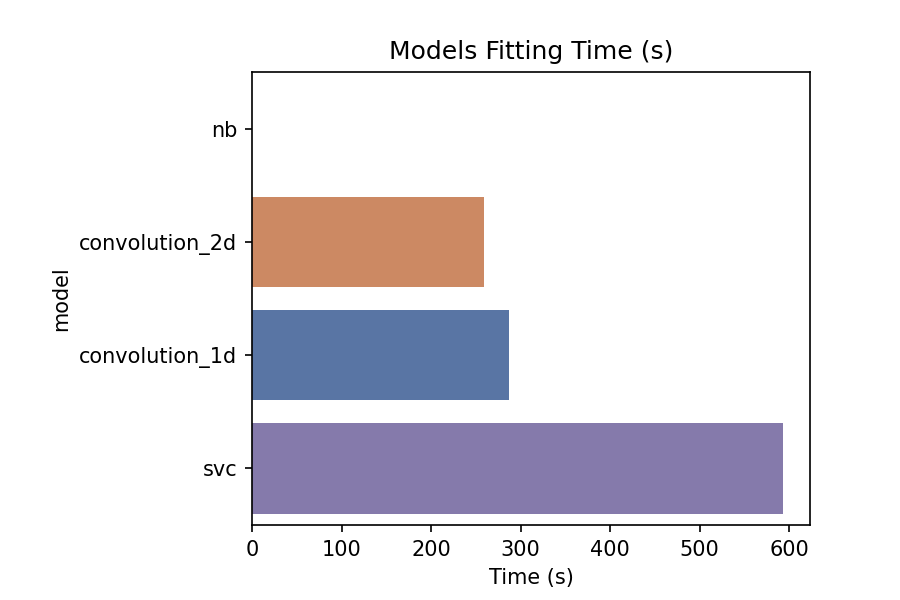
\includegraphics[width=16cm]{archivos/5.Resultados/TiemposEntrenamiento}
      \caption{Comparación entre los tiempos de entrenamiento de los modelos.}
      \label{TiemposEntrenamientoImage}
    \end{figure}

  
  \subsection{Gráficas de entrenamiento}

    Explicar las gráficas de evolución F1-score de las redes neuronales.


    \begin{figure}[h]
        \centering
        \includesvg[scale=0.3]{archivos/5.Resultados/CNN/1D/F1Score1D}
        \caption{Comparación de TODO(tipo) F1 score en validación y test CNN-1D.}
        \label{F1Score1DImage}
     \end{figure}


    \begin{figure}[h]
        \centering
        \includesvg[scale=0.3]{archivos/5.Resultados/CNN/2D/F1Score2D}
        \caption{Comparación de TODO(tipo) F1 score en validación y test CNN-2D.}
        \label{F1Score2DImage}
     \end{figure}


  \subsection{Reportes de clasificación}
       
    Explicar los reportes de clasificación con datos de \textbf{ENTRENAMIENTO.}

      \begin{table}[H]
        \centering
        \csvautotabular{archivos/5.Resultados/CNN/1D/1DClassificationReportTrain.csv}
        \caption{Métricas CNN-1D.}
        \label{CNN1DMetrics}
      \end{table}

      \begin{table}[H]
        \centering
        \csvautotabular{archivos/5.Resultados/NB/NBClassificationReportTrain.csv}
        \caption{Métricas Naive Bayes.}
        \label{NBMetrics}
      \end{table}

      \begin{table}[H]
        \centering
        \csvautotabular{archivos/5.Resultados/SVC/SVCClassificationReportTrain.csv}
        \caption{Métricas SVC.}
        \label{SVCDMetrics}
      \end{table}

      \begin{table}[H]
        \centering
        \csvautotabular{archivos/5.Resultados/KNN/KNNClassificationReportTrain.csv}
        \caption{Métricas SVC.}
        \label{SVCDMetrics}
      \end{table}

      \begin{table}[H]
        \centering
        \csvautotabular{archivos/5.Resultados/CNN/2D/2DClassificationReportTrain.csv}
        \caption{Métricas CNN-2D.}
        \label{CNN2DMetrics}
      \end{table}



  \subsection{Matrices de confusión}

    Explicar las matrices de confusión con datos de \textbf{ENTRENAMIENTO.}

    \begin{figure}
        \centering
        \begin{subfigure}[b]{0.4\textwidth}
            \centering
            \includesvg[scale=0.4]{archivos/5.Resultados/CNN/1D/1DConfusionMatrixTrain}
            \caption{Matriz de confusión CNN-1D.}
            \label{ConfusionMatrixTrainImages:1D}
        \end{subfigure}
        % Añadir el espacio deseado, si se deja la linea en blanco la siguiente subfigura ira en una nueva linea
        \begin{subfigure}[b]{0.4\textwidth}
            \centering
            \includesvg[scale=0.4]{archivos/5.Resultados/CNN/2D/2DConfusionMatrixTrain}
            \caption{Matriz de confusión CNN-2D.} 
            \label{ConfusionMatrixTrainImages:2D}

        \end{subfigure}
        \begin{subfigure}[b]{0.4\textwidth}
            \centering
            \includesvg[scale=0.4]{archivos/5.Resultados/NB/NBConfusionMatrixTrain}
            \caption{Matriz de confusión NB.}
            \label{ConfusionMatrixTrainImages:NB}
        \end{subfigure}

        \begin{subfigure}[b]{0.4\textwidth}
            \centering
            \includesvg[scale=0.4]{archivos/5.Resultados/KNN/KNNConfusionMatrixTrain}
            \caption{Matriz de confusión KNN.}
            \label{ConfusionMatrixTrainImages:KNN}
        \end{subfigure}

        \begin{subfigure}[b]{0.4\textwidth}
            \centering
            \includesvg[scale=0.4]{archivos/5.Resultados/SVC/SVCConfusionMatrixTrain}
            \caption{Matriz de confusión SVC.}
            \label{ConfusionMatrixTrainImages:SVC}
        \end{subfigure}

        \caption{Matrices de confusión de los modelos sobre el conjunto de entrenamiento.}
        \label{ConfusionMatrixTrainImages}
     \end{figure}

  \subsection{Comparativa entre modelos}

    Explicar la comparativa de modelos con datos de \textbf{ENTRENAMIENTO.}


    \begin{figure}[h]
        \centering
        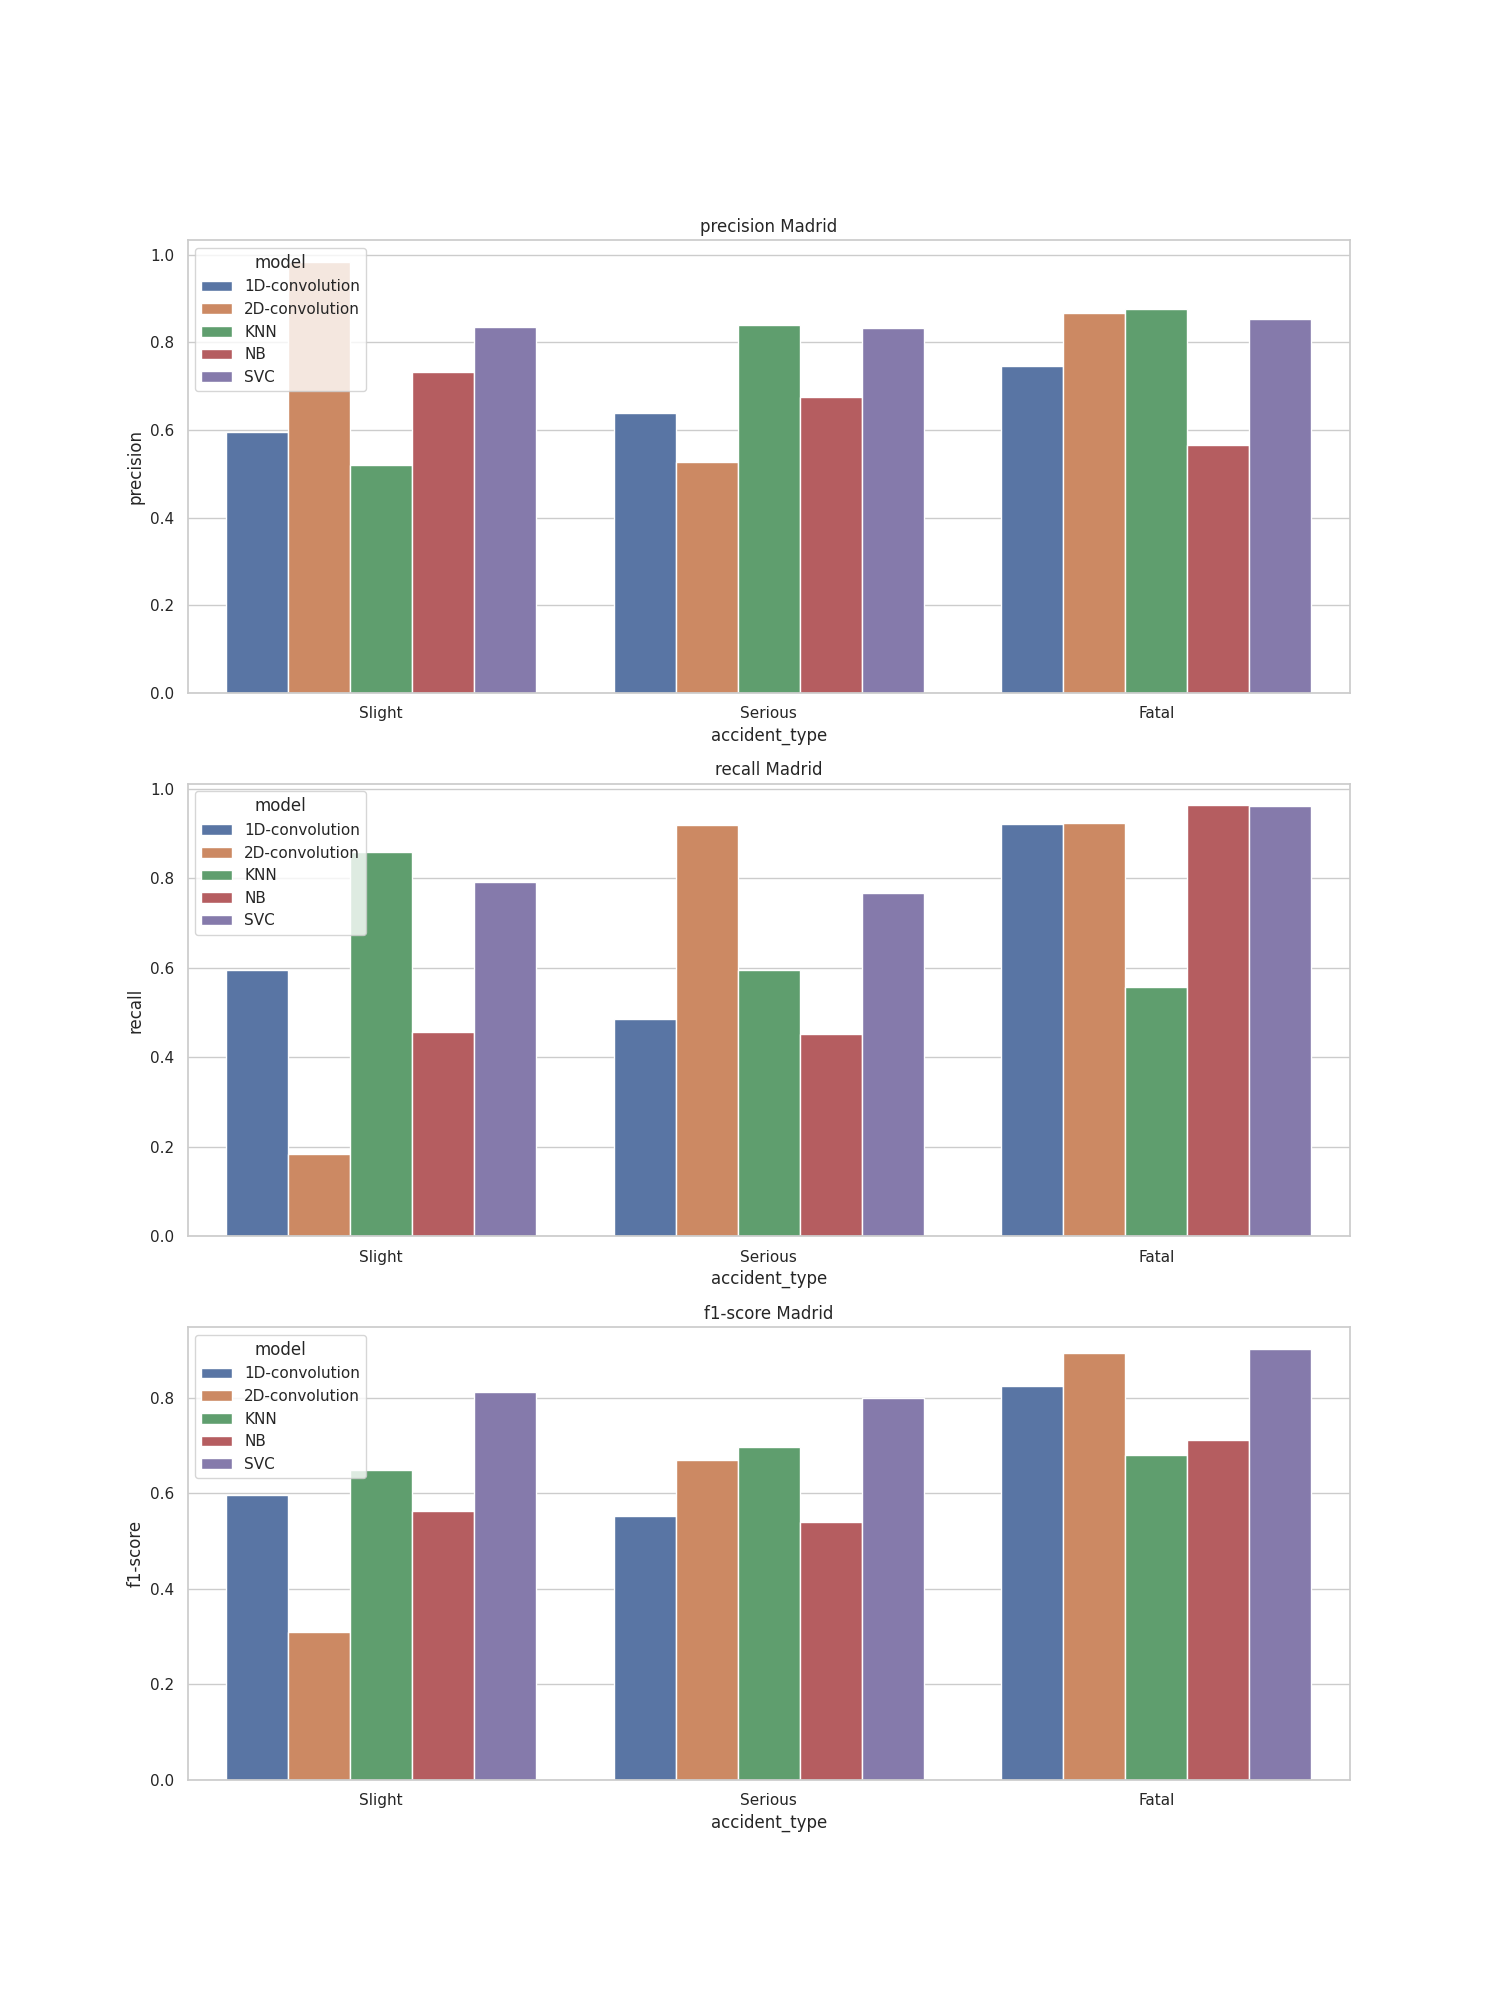
\includegraphics[width=16cm]{archivos/5.Resultados/ComparativaTrain}
        \caption{Comparativa de las métricas de las predicciones sobre el conjunto de entrenamiento de los modelos.}
        \label{ResultsTrainImage}
     \end{figure}



\section{Predicciones de modelos}

  \subsection{Reportes de clasificación}

    Explicar los reportes de clasificación con datos de \textbf{TEST.}

    \begin{table}[H]
      \centering
      \csvautotabular{archivos/5.Resultados/CNN/1D/1DClassificationReportTest.csv}
      \caption{Métricas CNN-1D.}
      \label{CNN1DMetrics}
    \end{table}

    \begin{table}[H]
      \centering
      \csvautotabular{archivos/5.Resultados/NB/NBClassificationReportTest.csv}
      \caption{Métricas Naive Bayes.}
      \label{NBMetrics}
    \end{table}

    \begin{table}[H]
      \centering
      \csvautotabular{archivos/5.Resultados/SVC/SVCClassificationReportTest.csv}
      \caption{Métricas SVC.}
      \label{SVCDMetrics}
    \end{table}

    \begin{table}[H]
      \centering
      \csvautotabular{archivos/5.Resultados/KNN/KNNClassificationReportTest.csv}
      \caption{Métricas SVC.}
      \label{SVCDMetrics}
    \end{table}

    \begin{table}[H]
      \centering
      \csvautotabular{archivos/5.Resultados/CNN/2D/2DClassificationReportTest.csv}
      \caption{Métricas CNN-2D.}
      \label{CNN2DMetrics}
    \end{table}

  \subsection{Matrices de confusión}

    Explicar las matrices de confusión con datos de \textbf{TEST.}

    \begin{figure}
        \centering
        \begin{subfigure}[b]{0.4\textwidth}
            \centering
            \includesvg[scale=0.4]{archivos/5.Resultados/CNN/1D/1DConfusionMatrixTest}
            \caption{Matriz de confusión CNN-1D.}
            \label{ConfusionMatrixTestImages:1D}
        \end{subfigure}
        % Añadir el espacio deseado, si se deja la linea en blanco la siguiente subfigura ira en una nueva linea
        \begin{subfigure}[b]{0.4\textwidth}
            \centering
            \includesvg[scale=0.4]{archivos/5.Resultados/CNN/2D/2DConfusionMatrixTest}
            \caption{Matriz de confusión CNN-2D.} 
            \label{ConfusionMatrixTestImages:2D}

        \end{subfigure}
        \begin{subfigure}[b]{0.4\textwidth}
            \centering
            \includesvg[scale=0.4]{archivos/5.Resultados/NB/NBConfusionMatrixTest}
            \caption{Matriz de confusión NB.}
            \label{ConfusionMatrixTestImages:NB}
        \end{subfigure}

        \begin{subfigure}[b]{0.4\textwidth}
            \centering
            \includesvg[scale=0.4]{archivos/5.Resultados/KNN/KNNConfusionMatrixTest}
            \caption{Matriz de confusión KNN.}
            \label{ConfusionMatrixTestImages:KNN}
        \end{subfigure}

        \begin{subfigure}[b]{0.4\textwidth}
            \centering
            \includesvg[scale=0.4]{archivos/5.Resultados/SVC/SVCConfusionMatrixTest}
            \caption{Matriz de confusión SVC.}
            \label{ConfusionMatrixTestImages:SVC}
        \end{subfigure}

        \caption{Matrices de confusión de los modelos sobre el conjunto de entrenamiento.}
        \label{ConfusionMatrixTestImages}
     \end{figure}

  \subsection{Comparativa entre modelos}

    Explicar la comparativa de modelos con datos de \textbf{ENTRENAMIENTO.}


    \begin{figure}[h]
        \centering
        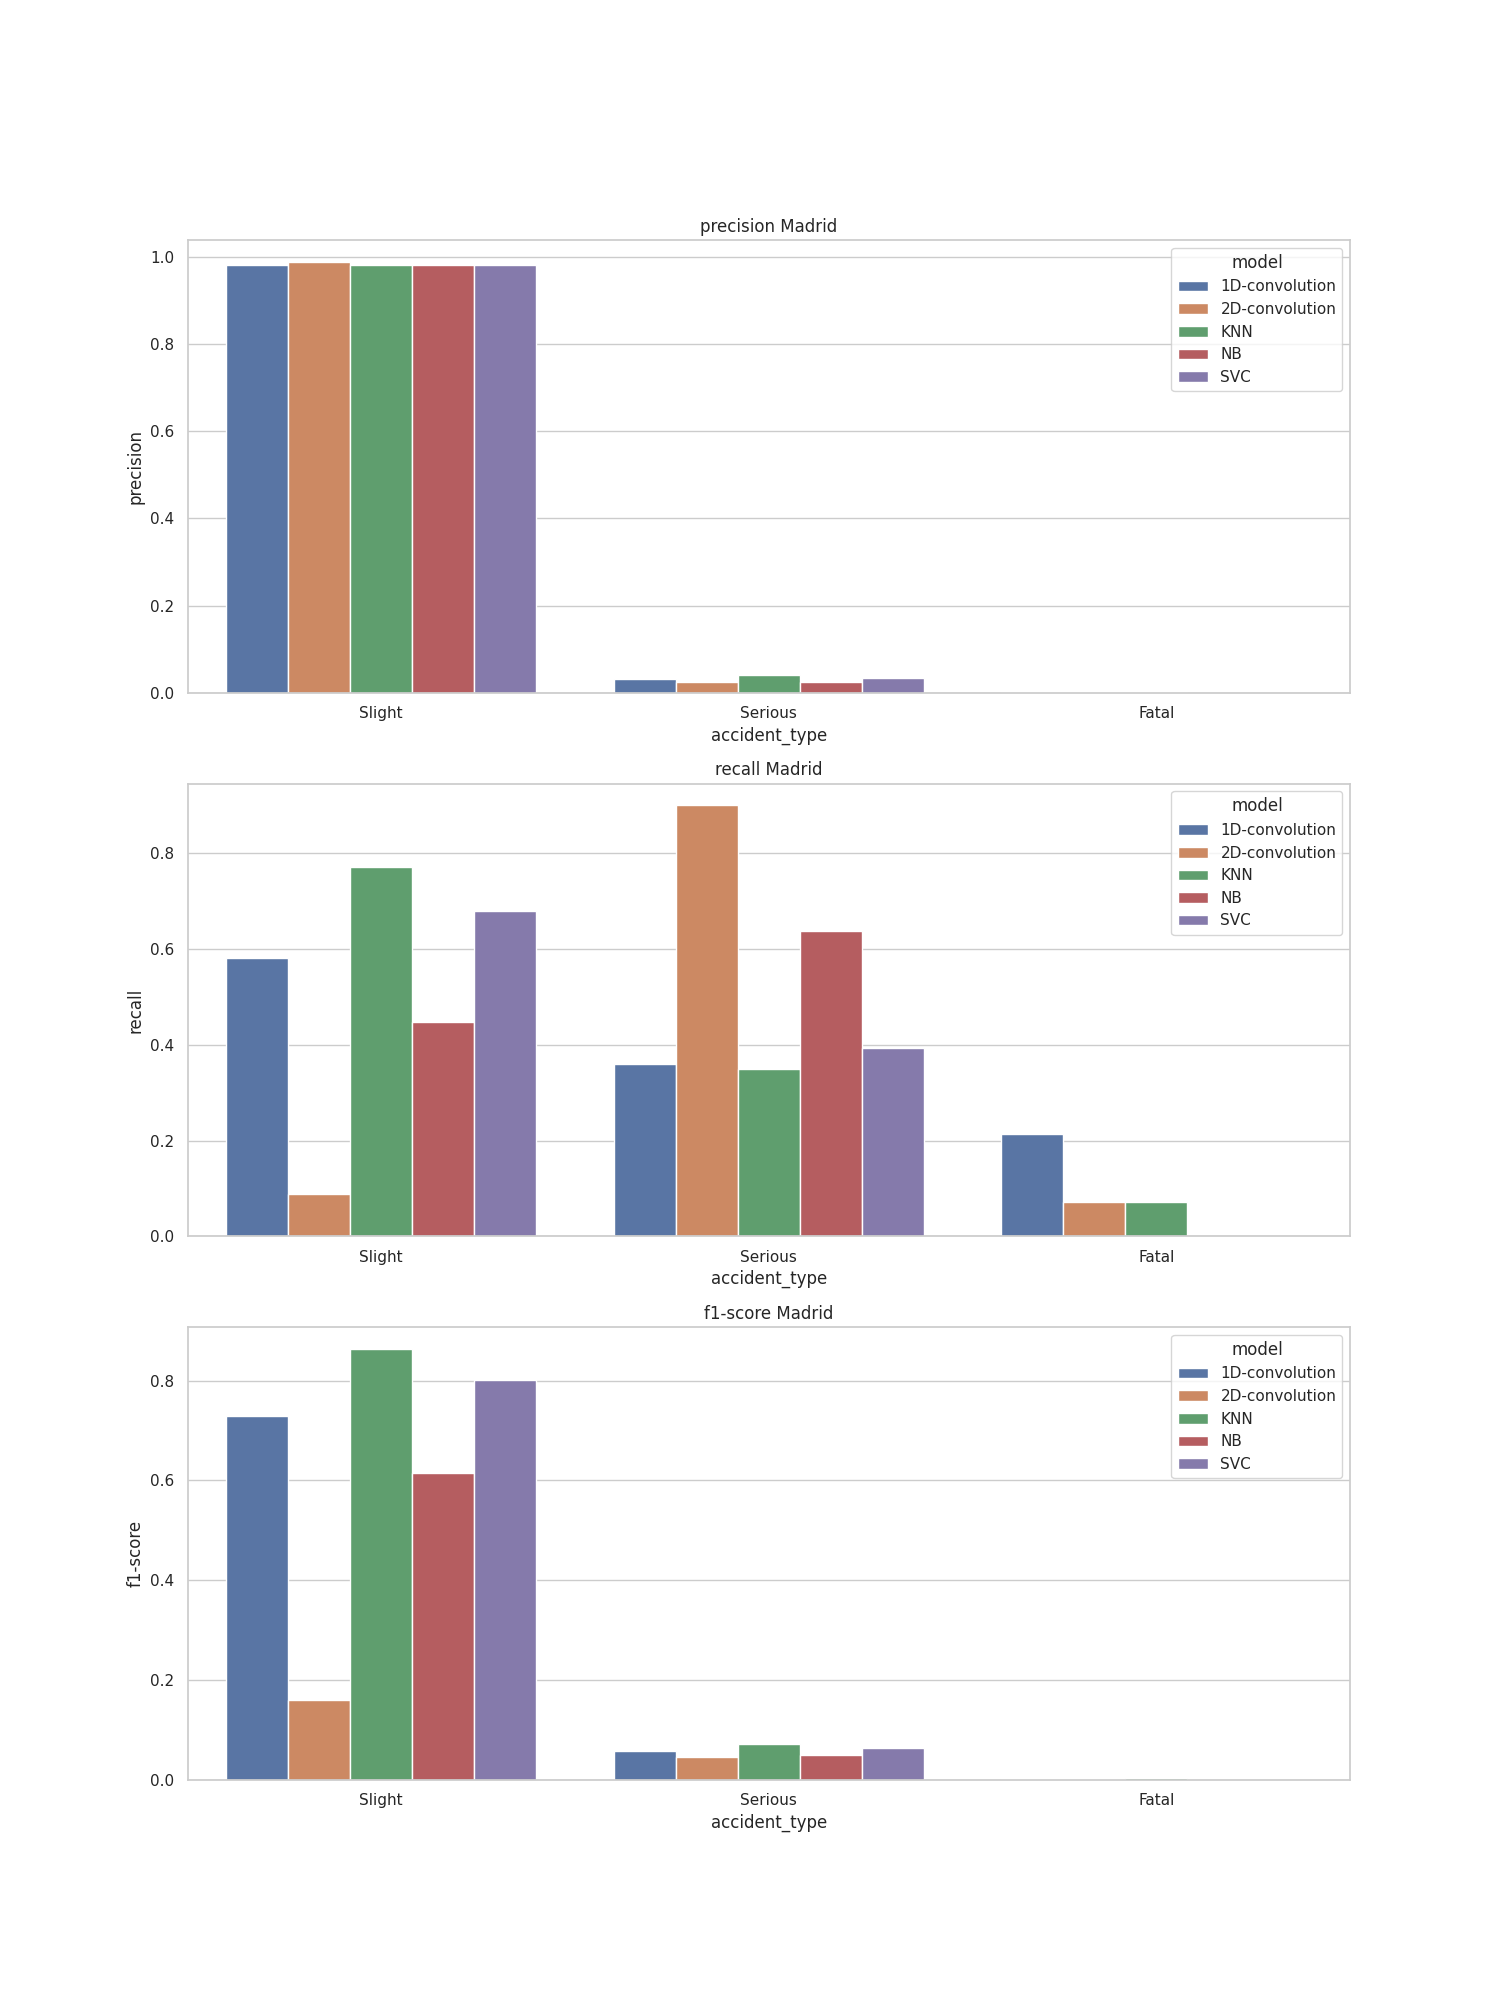
\includegraphics[width=16cm]{archivos/5.Resultados/ComparativaTest}
        \caption{Comparativa de las métricas de las predicciones sobre el conjunto de test de los modelos.}
        \label{ResultsTestImage}
     \end{figure}



Como podemos observar, los modelos entrenados predicen bien sus muestras de enrenamiento sin embargo inguno de los modelos aplicados es capaz de generalizar bien sore el conjunto de datos de test sin smote
esto es debido a la naturaleza de los datos, de la informacio que tenemos y de el tipo de limpieza que se ha hecho. Se ppodria hacer un estudio del valor numerico que se le asigna a cada variable en la limpieza, ya que seguramente al estar nosotros haciendolo aleatoriamente seguramente se esté creando algún patrón de jerarquía dentro de una columna o se le da mas importancia a un todoterreno que a un avion porque el todoterrento al tener un valor asignado más alto sera mas negro y por lo tanto la red predicira lo que sea		% Plantilla: Se muestran gráficas
%%%%%%%%%%%%%%%%%%%%%%%%%%%%%%%%%%%%%%%%%%%%%%%%%%%%%%%%%%%%%%%%%%%%%%%%
% Plantilla TFG/TFM
% Escuela Politécnica Superior de la Universidad de Alicante
% Realizado por: Jose Manuel Requena Plens
% Contacto: info@jmrplens.com / Telegram:@jmrplens
%%%%%%%%%%%%%%%%%%%%%%%%%%%%%%%%%%%%%%%%%%%%%%%%%%%%%%%%%%%%%%%%%%%%%%%%

\chapter{Conclusiones}
\label{conclusiones}



\section{Líneas de investigación}


	Teniendo en cuenta los resultados de los experimentos, existen múltiples líneas de investigación en las que seguir desarrollando el proyecto de cara a obtener un mejor rendimiento:

	\begin{enumerate}


		\item Las transformaciones sobre las variables del dataset son un punto crítico, por lo que es necesario realizar un estudio de las mismas para probar si otras tipificaciones sobre las variables tienen un efecto positivo en el rendimiento de las clasificaciones. Un ejemplo de este caso es la variable \textit{hora}, que puede ser transformada de acuerdo a otro rango de horas para declarar si un accidente se ha producido de día o de noche o modificar la tipificación del rango de edad. Estos cambios afectaría notablemente a los árboles de decisión producidos por \glsentryshort{xgboost}.

		\item Se propone también usar herramientas como \textit{Open Refine} \cite{OpenRefine} que permitan realizar clústers nominales sobre la localización de los accidentes para obtener una tipificación más sólida del tipo de carretera.

		\item Otra de las líneas a investigar es el añadido de características provenientes de otros datasets localizados en el portal de datos abiertos de la ciudad de Madrid. Dichos datasets proveen de información tal como la velocidad media de los tramos, la densidad de tráfico o la temperatura ambiente. Estos posibles futuros predictores pueden ser claves para la clasificación, como por ejemplo las bajas temperaturas que afectan al agarre de los neumáticos.

		\item Como siguiente opción se propone aumentar el número de características del dataset en base a las propias variables del conjunto de datos original, realizando más transformaciones que permitan obtener más predictores. Por ejemplo el mes, día y estación del año en el que se ha producido el accidente en base a la hora.

		\item En lo que respecta a los algoritmos sería conveniente ampliar los hiperparámetros a utilizar por \glsentryshort{xgboost}, optimizándolos además mediante le algoritmo genético. En este proyecto se optimizan tres de ellos debido a las limitaciones computacionales, mientras que existen otros como \textit{gamma} (parámetro de reducción mínima) \textit{hojas máximas} (parámetro de regularización) o la \textit{política de crecimiento} (controla la forma en la que los nuevos nodos se añaden al árbol) entre otros.

		\item Otro enfoque consistiría estudiar alguna otra técnica para formar matrices en base a representaciones tabulares de datos, maximizando la información de los accidentes en base a la posición de las características.

		\item Utilizar metaaprendizaje para entrenar modelos que averiguen los mejores hiperparametros para otros modelos

		\item En lo que respecta al remuestreo de datos sería conveniente a analizar distintos métodos de remuestreo además de \textit{Undersampling, Oversampling y SMOTE} ya estudiados. Existen numerosos parámetros de \glsentryshort{smoteii} que pueden ser configurados, entrenando los modelos con este nuevo remuestreo de datos sería posible aumentar el rendimiento de los mismos.

		\item Utilizar técnicas de \textit{Automated Machine Learning} como \glsentryfull{nas} como AutoKeras \cite{AutoKeras} para encontrar la mejor estructura de la red para el problema. Las \glsentryshort{nas} buscan encontrar una arquitectura neuronal óptima basándose en ensayo y error. Este tipo de técnias requiere grandes recursos computacionales, por lo que para poder llevarla a cabo es necesario disponer de sistema con grandes capacidades de cómputo en \textit{GPU}.


	\end{enumerate}	% Plantilla: Se muestran matemáticas

%%%%
% CONTENIDO. BIBLIOGRAFÍA.
%%%%

\nocite{*} %incluye TODOS los documentos de la base de datos bibliográfica sean o no citados en el texto

\newpage
\bibliography{bibliografia/bibliografia} % Archivo que contiene la bibliografía
\bibliographystyle{IEEEtran}

%%%%
% CONTENIDO. LISTA DE ACRÓNIMOS. Comenta las líneas si no lo deseas incluir.
%%%%
% Incluye el listado de acrónimos utilizados en el trabajo. 
\printglossary[style=modsuper,type=\acronymtype,title={Lista de Acrónimos y Abreviaturas}]
% Añade el resto de acrónimos si así se desea. Si no elimina el comando siguiente
\glsaddallunused 

%%%%
% CONTENIDO. Anexos - Añade o elimina según tus necesidades
%%%%


\end{document}
